%% Bayesian Networks Research

\documentclass[11pt,a4paper]{report}

%%------------------------------- preamble ------------------------------------

%% comment next for EN
\usepackage[utf8]{inputenc}       % accents
\usepackage[T1]{fontenc}          % PS fonts
\usepackage{newtxtext,newtxmath}  % do not use CM fonts
\usepackage{amsmath}              % multi-line and other mathematical statements
\usepackage{setspace}             % setting the spacing between lines
\usepackage{graphicx}             % go far beyond what the graphics package
\usepackage[normalem]{ulem}       % various types of underlining
\usepackage{caption}              % rotating captions, sideways captions, etc.
\usepackage{float}                % tables and figures in the multi-column environment 
\usepackage{subcaption}           % for subfigures and the like
\usepackage{longtable}            % tables that continue to the next page
\usepackage{multirow}             % tabular cells spanning multiple rows
\usepackage[table]{xcolor}        % driver-independent color extensions
\usepackage{lipsum}               % loren dummy text
\setlength{\marginparwidth}{2cm}  % todonotes' requirements
\usepackage{todonotes}            % todo's
\usepackage{chicago}              % a bibliography style
\usepackage{tabularx}
\usepackage{graphicx}
%% document dimensions
\usepackage[a4paper,left=25mm,right=25mm,top=25mm,bottom=25mm,headheight=6mm,footskip=12mm]{geometry}
\setlength{\parindent}{0em}
\setlength{\parskip}{1ex}

%% headers & footers
\usepackage{lastpage}
\usepackage{fancyhdr}
\fancyhf{}                            % clear off all default fancyhdr headers and footers
\rhead{\small{\emph{\projtitle, \projauthor}}}
\rfoot{\small{\thepage\ / \pageref{LastPage}}}
\pagestyle{fancy}                     % apply the fancy header style
\renewcommand{\headrulewidth}{0.4pt}
\renewcommand{\footrulewidth}{0.4pt}

%% colors
\usepackage{color}
\definecolor{engineering}{rgb}{0.549,0.176,0.098}
\definecolor{cloudwhite}{cmyk}{0,0,0,0.025}

%% source-code listings
\usepackage{listings}
\lstset{ %
 language=Python,                        % choose the language of the code
 basicstyle=\footnotesize\ttfamily,
 keywordstyle=\bfseries,
 numbers=left,                      % where to put the line-numbers
 numberstyle=\scriptsize\texttt,    % the size of the fonts that are used for the line-numbers
 stepnumber=1,                      % the step between two line-numbers. If it's 1 each line will be numbered
 numbersep=8pt,                     % how far the line-numbers are from the code
 frame=tb,
 float=htb,
 aboveskip=8mm,
 belowskip=4mm,
 backgroundcolor=\color{cloudwhite},
 showspaces=false,                  % show spaces adding particular underscores
 showstringspaces=false,            % underline spaces within strings
 showtabs=false,                    % show tabs within strings adding particular underscores
 tabsize=2,                         % sets default tabsize to 2 spaces
 captionpos=b,                      % sets the caption-position to bottom
 breaklines=true,                   % sets automatic line breaking
 breakatwhitespace=false,           % sets if automatic breaks should only happen at whitespace
 escapeinside={\%*}{*)},            % if you want to add a comment within your code
 morekeywords={*,var,template,new}  % if you want to add more keywords to the set
}

%% hyperreferences (HREF, URL)
\usepackage{hyperref}
\hypersetup{
    plainpages=false, 
    pdfpagelayout=SinglePage,
    bookmarksopen=false,
    bookmarksnumbered=true,
    breaklinks=true,
    linktocpage,
    colorlinks=true,
    linkcolor=engineering,
    urlcolor=engineering,
    filecolor=engineering,
    citecolor=engineering,
    allcolors=engineering
}

%% path to the figures directory
\graphicspath{{figures/}}

%% macros, to be updated as needed
\newcommand{\school}{}
\newcommand{\degree}{}
\newcommand{\projtitle}{Bayesian Networks I: BN Representation}
\newcommand{\subtitle}{For Self-learning Purposes}
\newcommand{\projauthor}{Jiashu Chen}
\newcommand{\supervisor}{}
\newcommand{\tutor}{}

%% my other macros, if needed
\newcommand{\windspt}{\textsf{WindsPT\/}}
\newcommand{\windscannerpt}{\emph{Windscanner.PT\/}}
\newcommand{\class}[1]{{\normalfont\slshape #1\/}}
\newcommand{\svg}{\class{SVG}}
\newcommand{\mycomment}[1]{}

\graphicspath{ {./pics/} }

%% my environments for infos
\newenvironment{info}[1]{\vspace*{6mm}\color{blue}[ \textbf{INFO:} \begin{em} #1}
                        {\vspace*{3mm}\end{em} ]}
\newenvironment{infoopt}[1]{\vspace*{6mm}\color{blue}[ \textbf{INFO (elemento opcional):} \begin{em} #1}
                        {\vspace*{3mm}\end{em} ]}

%%------------------------------- document-------------------------------------

\begin{document}

%% preamble page numbers with roman numerals
\pagenumbering{roman}\setcounter{page}{1}
\pagestyle{plain}

%%------------------------------- cover page ----------------------------------

\begin{titlepage}
\center

\vspace{-15mm}
{\large \textbf{\textsc{\school}}}\\

\vfill

{\Large \textbf{\projtitle}}\\[8mm]
{\large \textbf{\subtitle}}\\[28mm]

{\Large \textbf{\projauthor}}\\

\vfill

%% includegraphics[width=52mm]{uporto-feup.pdf}

\vfill

%% {\large \degree}\\[8mm]
%\renewcommand{\today}{15 de dezembro de 2023}
\today

\end{titlepage}

%%------------------------------- table of contents ---------------------------

\tableofcontents

%%------------------------------- chapter ------------------------------------

\chapter{Joint Distribution}

%% display headers & footers
\pagestyle{fancy}
%% main page numbers with arabic numerals
\pagenumbering{arabic}\setcounter{page}{1}

\section{Covid Example: 12 Data Sample}

\begin{center}
    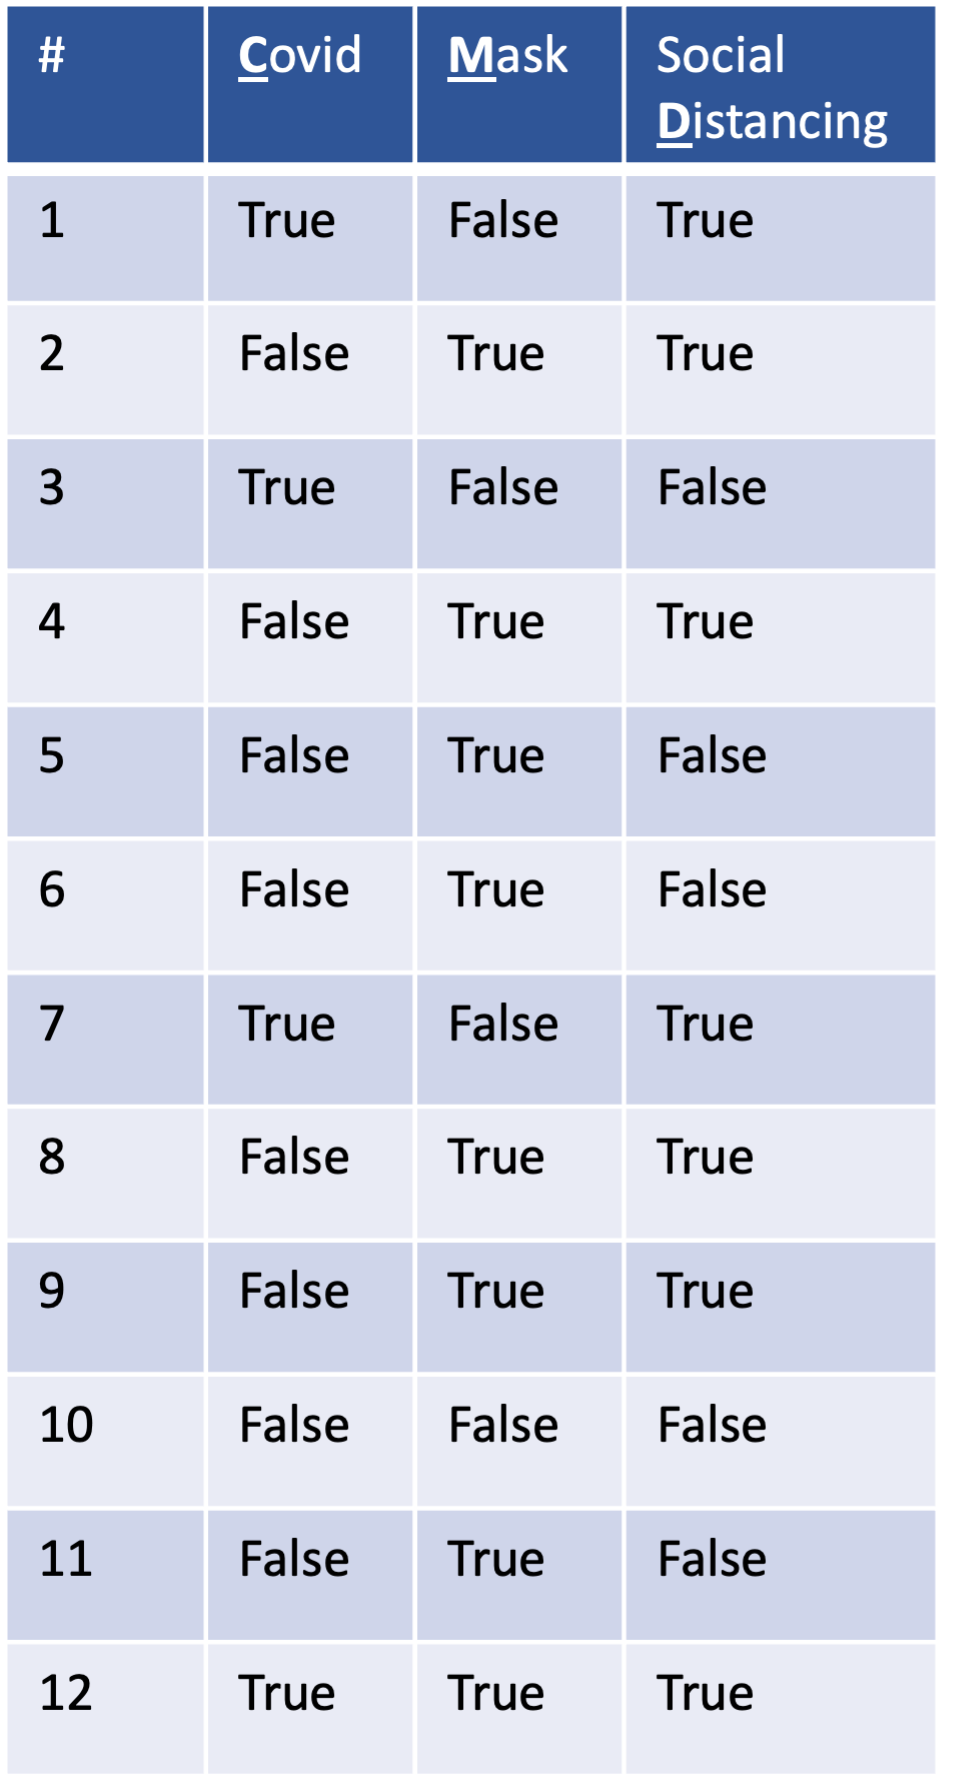
\includegraphics[width=4cm, height=8cm]{covid_3var.png}
\end{center}

\mycomment{
\begin{center}
    \begin{tabular}{||c c c c||} 
     \hline
     \# & COVID & Mask & Social Distancing \\ [0.5ex] 
     \hline\hline
     1 & True & False & True \\ 
     \hline
     2 & False & True & True \\
     \hline
     3 & True & False & False \\
     \hline
     4 & False & True & True \\
     \hline
     5 & False & True & True \\
     \hline
     6 & False & True & False \\
     \hline
     7 & True & False & True \\
     \hline
     8 & False & True & True \\
     \hline
     9 & False & True & True \\
     \hline
     10 & False & False & False \\
     \hline
     11 & False & True & False \\
     \hline
     12 & True & True & True \\ [1ex] 
     \hline
    \end{tabular}
\end{center}
}

\begin{equation}
    P(COVID = F \mid Mask = T, Social Distancing = T) = ?
\end{equation}

\begin{itemize}
\item Marginal Probability

\begin{equation}
    \begin{split}
    P(M = T, D = T) & = \sum_{C = T, F} P(C, M = T, D = T) = \frac{6}{12}
    \end{split}
\end{equation}

\item Conditional Probability
    
\begin{equation}
    \begin{split}
    P(C = F \mid M = T, D = T) & = \frac{P(C = F, M = T, D = T)}{P(M = T, D = T)} \\
    & = \frac{5/12}{6/12}
    \end{split}
\end{equation}

\item Joint Probability Distribution

The key is to find the joint probability distribution for C, M, D, i.e.,
$P(C, M, D)$, with 8 parameters p1, \ldots, p8, where $\sum_{i=1}^{8} p_{i} = 1$

So, the number of parameters to obtain $P(C, M, D)$ is $2^{3} - 1 = 7$
\end{itemize}

\textbf{\color{blue}Key Takeaways}: \\ \textit{\color{blue}If we have the joint distribution, we can calculate any probability using conditional distribution and marginal distribution.}

\section{Probability}

\begin{itemize}
    \item Joint probability distribution
    \begin{center}
        $P(X_{1}, X_{2}, \ldots, X_{n})$
    \end{center}

    \item Marginal probability distribution
    
    Marginalize out some variables
    \begin{center}
        $P(X_{1}) = \sum_{x_{2} \ldots x_{n}} P(X_{1}, X_{2}, \ldots, X_{n})$
    \end{center}

    \item Conditional probability distribution
    \begin{center}
        $P(X_{1} \mid X_{2} \ldots X_{n}) = \frac{P(X_{1} X_{2} \ldots X_{n})}{P(X_{2} \ldots X_{n})}$
    \end{center}

    \item Number of parameters of a distribution

    Given discrete random variables $X_{1} X_{2} \ldots X_{n}$ that take $\alpha_{1}, \alpha_{2}, \ldots, \alpha_{n}$ values, respectively, 
    
    \begin{itemize}
        \item  the number of parameters to represent $P(X_{1}X_{2} \ldots X_{n})$ is 
        \begin{center}
            $ \alpha_{1} \alpha_{2} \ldots \alpha_{n} - 1$
        \end{center}

        \item  the number of parameters to represent $P(X_{1} \mid X_{2} \ldots X_{n})$ is 
        \begin{center}
            $ (\alpha_{1} - 1) \alpha_{2} \ldots \alpha_{n}$
        \end{center}

    \end{itemize}
\end{itemize}

\section{Summary: What is the Goal?}

The goal is to find the joint probability distribution from data. So that we could answer any probablistic inqueries.
\begin{center}
    $P(C, M, D) = ?$
\end{center}

\begin{center}
    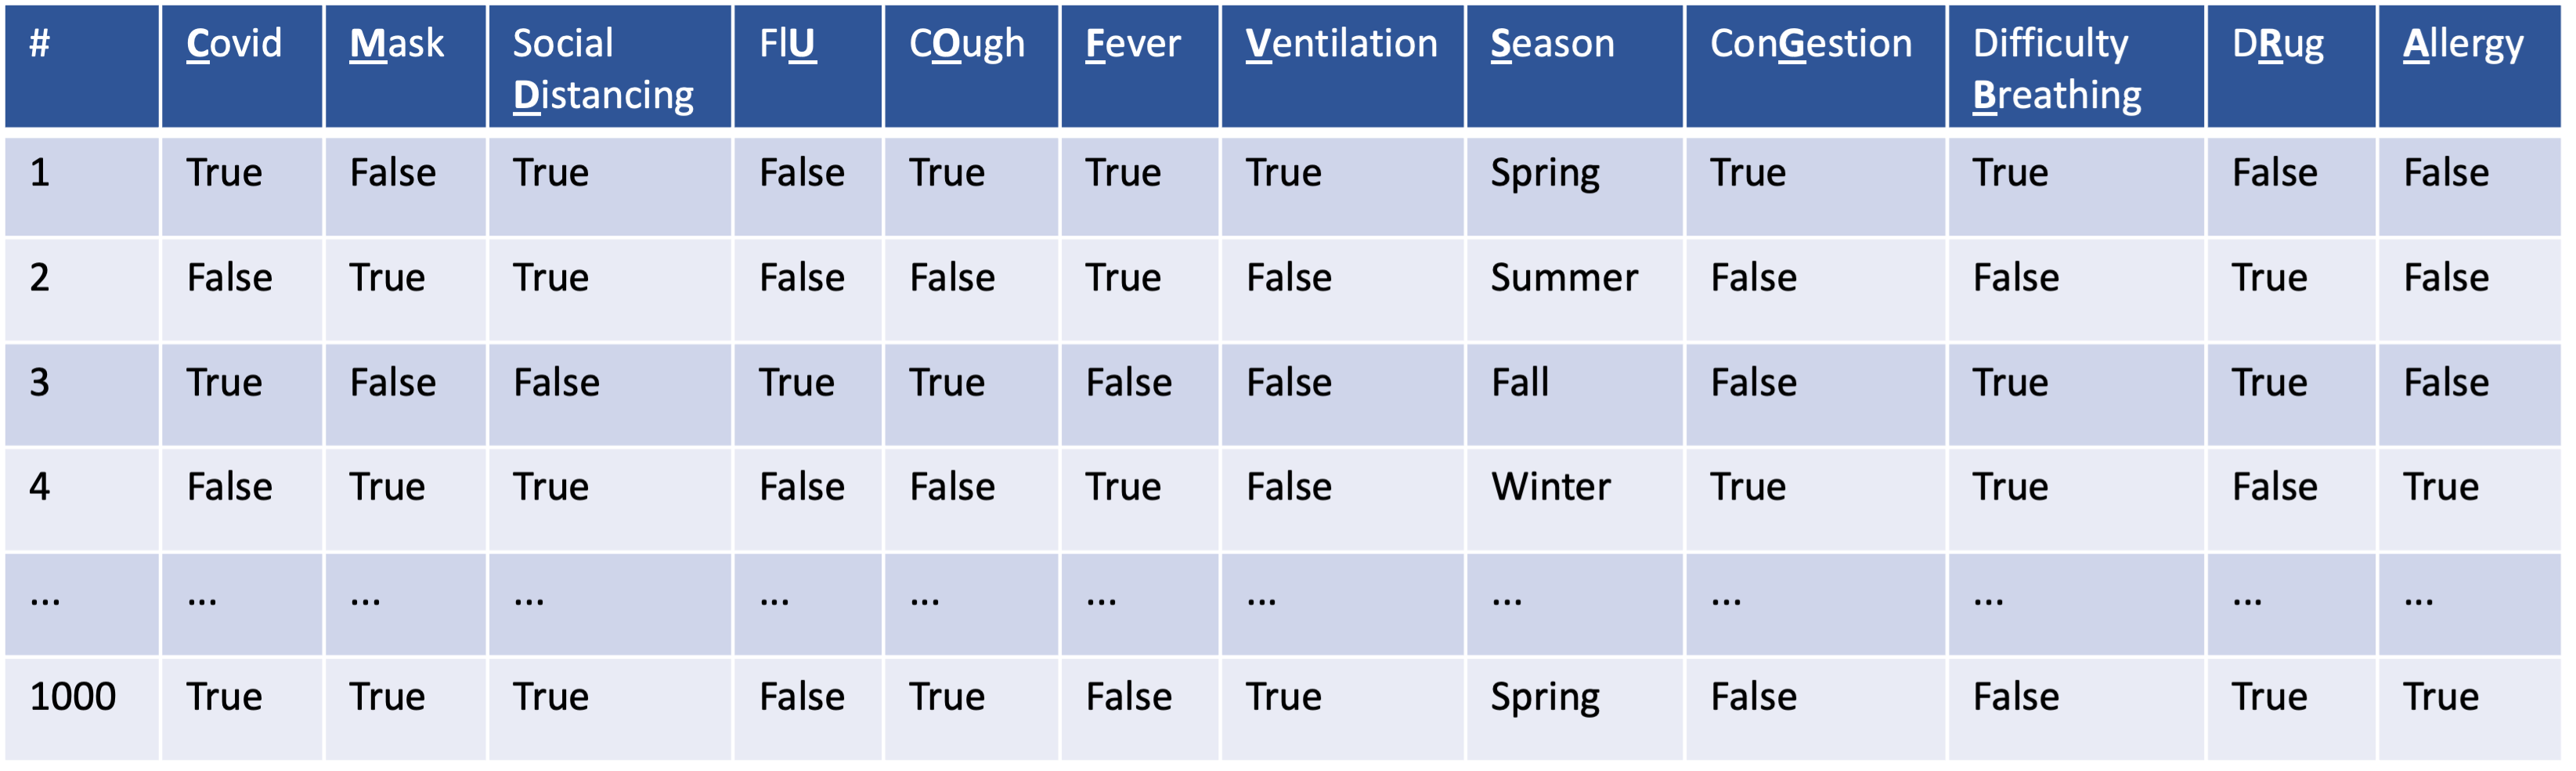
\includegraphics[width=15cm, height=4cm]{covid_12var.png}
\end{center}

However, in the real world, we often have much more variables. Suppose we have 12 variables in the covid example, all binary except for season with 4 values, then the number of required parameters to calculate joint probability is $2^{11} * 4 - 1 = 8191$

If we only have 1000 data points, then we have to set at least 7191 parameters to zero, which is problematic.

%%------------------------------- chapter ------------------------------------

\chapter{Independence}

So we understand the importance of joint probability distribution, the problem now is to deal with the large number of parameters while calculating joint probability distribution.

\section{Importance of Independence}

For Covid, Mask, Social Distancing, using conditional probability

\begin{center}
    $P(C, M, D) = P(C \mid M, D)P(M, D)$
\end{center}

Suppose M and D are independent, denoted by $M \perp D$,

\begin{center}
    $P(M, D) = P(M)P(D)$ \\
    Thus,
    $P(C, M, D) = P(C \mid M, D)P(M)P(D)$\\
    \vspace{0.5cm}
    $Number\ of\ parameters = 2^2 + (2 - 1) + (2 - 1) = 6$\\
    $P(C \mid M, D): (2-1) * 2 * 2 = 2^2$\\
    $P(M): M\ takes\ two\ values = 2$\\
    $P(D): D\ takes\ two\ values = 2$\\
    
\end{center}


\section{Statistical Independence}

Random variables X and Y are independent, i.e. $X \perp Y$, if
\begin{center}
    $P(X, Y) = P(X)P(Y)$ \\
    $or P(X \mid Y) = P(X) or P(Y \mid X) = P(Y) $
\end{center}

Covid Example

\begin{center}
    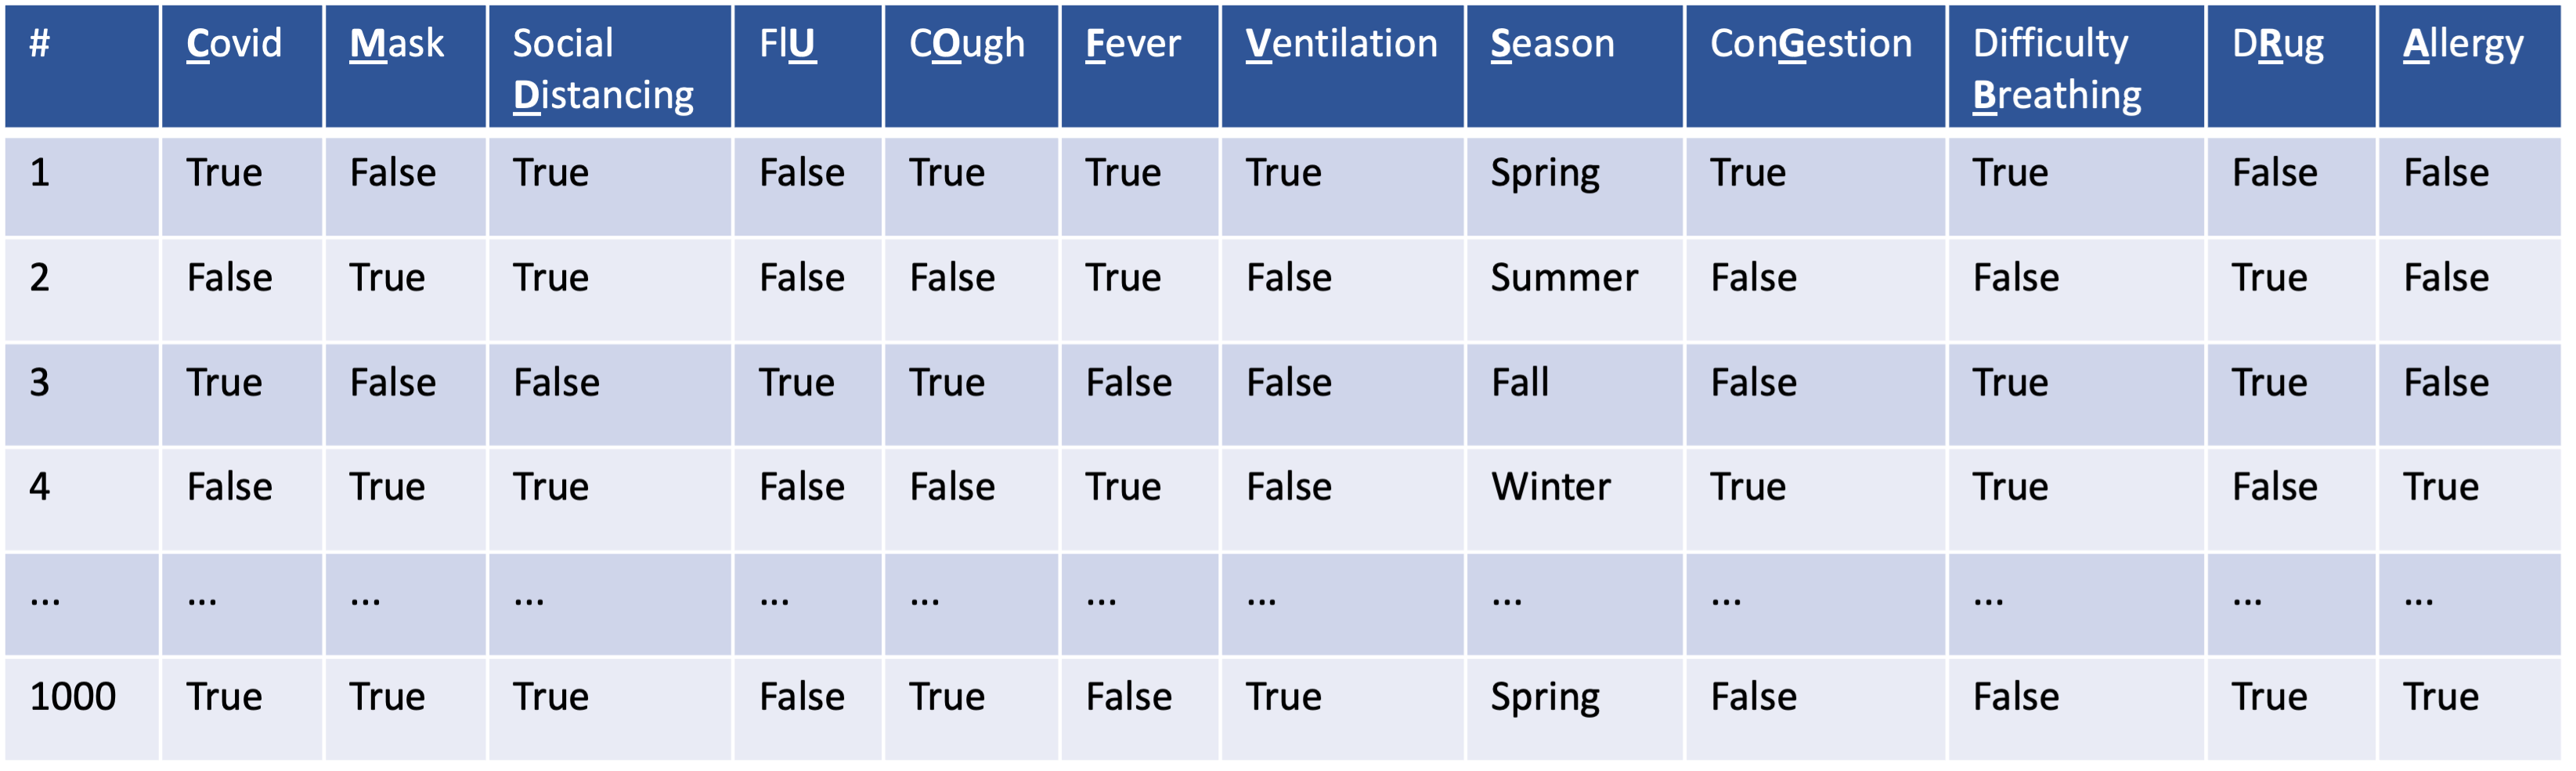
\includegraphics[width=15cm, height=4cm]{covid_12var.png}
\end{center}

Suppose all 12 random variables are mutually independent:

\begin{center}
    $C \perp M, C \perp D, \ldots, R \perp A$\\
    $P(C, M, D, U, \ldots, A) = P(C)P(M)P(D) \cdots P(A)$\\
    \vspace{0.5cm}
    $Number\ of\ parameters = 11 + 3 = 14$\\
    The previous number was 8191.
\end{center}

\begin{center}
    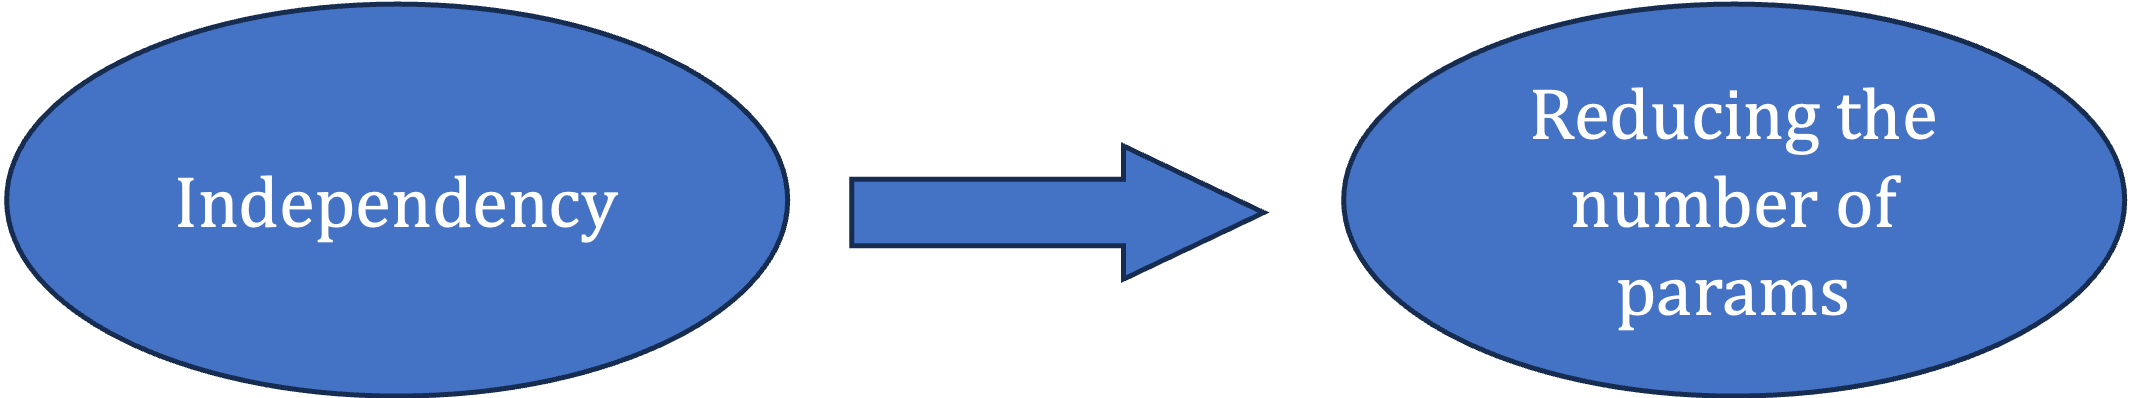
\includegraphics[width=10cm, height=2cm]{indep_red.png}
\end{center}

\textbf{\color{blue}Key Takeaways}: \\ \textit{\color{blue}with M,D being independent, the number of parameters reduced from 7 to 6. Therefore, independence could reduce the number of parameters.}

However, the independence assumption does not always hold. For instance, $Mask \not\!\perp\!\!\!\perp Social\ distancing$ 


\section{Conditional Independence}

\begin{itemize}
    \item Bother, Sister, Parent Example

\begin{itemize}
    \item Consider a brother(B) and a sister(S)\\
    $P(S = white \mid B = white) = 0.9$\\
    $P(S = white \mid B = black) = 0.1$\\
    Therefore, $S \not\!\perp\!\!\!\perp B$ 
    \item Consider brother(B), sister(S), and Parent(Pa)\\
    $P(S = white \mid Pa = white) = 0.95$\\
    $P(S = white \mid Pa = white, B = white) = 0.95$\\
    $P(S = white \mid Pa = white, B = black) = 0.95$\\
    \vspace{0.5cm}
    Therefore, knowing the brother does not matter if we know the parent\\
    \textbf{S is conditionally independent of B given Pa, i.e. $(S \perp B \mid Pa)$}
\end{itemize}

\item Conditional Independence Definition

Consider the set of random variables X, Y, Z,
We say that X is conditionally independent of Y given Z in a distribution P, denoted by $P \models (X \perp Y \mid Z)$ if
\begin{center}
    $P(X = x \mid Y = y, Z = z) = P(X = x \mid Z = z), \forall x,y,z$
\end{center}

\begin{itemize}
    \item The variables in set Z are said to be observed
    \item The set of all probability independencies in P is denoted by $I(P)$
    \begin{center}
        $P \models (X \perp Y \mid Z)\ if\ and\ only\ if$\\
        $P(X, Y \mid Z) = P(X \mid Z)P(Y \mid Z)$
    \end{center}
\end{itemize}
\item How can Conditional Independence Help

\begin{itemize}
    \item Using Covid, Fever, and PRC test example\\
    \begin{center}
        $P(F,P,C) = P(F \mid P,C)P(P,C)$\\
    \end{center}
    \item if $P(F \perp P \mid C) \in I(P)$, i.e. fever and prc test are conditionally independent given covid, then\\
    \begin{center}
        $P(F,P,C) = P(F \mid C)P(P,C)$
    \end{center}
    \item The number of parameters = $2 + (2**2 - 1) = 5$
\end{itemize}
\end{itemize}

\textbf{\color{blue}Key Takeaways}: \\ \textit{\color{blue}Conditional independence can reduce the number of parameters.}

\section{Conditional Independence with Chain Rule}

\begin{itemize}
    \item We could factor joint distribution into CPDs using chain rule

\begin{center}
    $P(X_{1},\ldots, X_{n}) = P(X_{n} \mid X_{n-1}, \ldots, X_{1}) \dots P(X_{3} \mid X_{2},X_{1})P(X_{2} \mid X_{1})P(X_{1})$\\
    $ = \prod_{i=1}^{n} p(X_{i} \mid X_{i-1}, \ldots, X_{1})$
\end{center}

Suppose all random variables take binary values, then the number of parameters for 
\begin{center}
    $p(X_{i} \mid X_{i-1}, \ldots, X_{1}) = 2^{(i-1)}$
\end{center}

\item Consider joint distribution P(X1, X2, X3, X4). Using the chain rule, we could ge
\begin{center}
    $P(X_{1}, X_{2}, X_{3}, X_{4}) = P(X_{4} \mid X_{3}, X_{2}, X_{1}) P(X_{3} \mid X_{2}, X_{1})P(X_{2} \mid X_{1})P(X_{1})$
\end{center}
\item If $(X_{4} \perp X_{1}, X_{2} \mid X_{3}) \in I(P)$, then
\begin{center}
    $P(X_{4} \mid X_{3}, X_{2}, X_{1}) = P(X_{4} \mid X_{3})$
\end{center}
\item The joint distribution becomes
\begin{center}
    $P(X_{1}, X_{2}, X_{3}, X_{4}) = P(X_{4} \mid X_{3}) P(X_{3} \mid X_{2}, X_{1})P(X_{2} \mid X_{1})P(X_{1})$
\end{center}
\item The total number of parameters reduced from $2^4 - 1 = 15$ to $2 + 2^2 + 2 + 1 = 9$
\end{itemize}

\section{Summary: What is the Goal?}

\begin{itemize}
    \item Now we know that to calculate joint probability distribution, we just need to find the conditional independencies and factorize the joint probability distribution. But, there are two more problems

\begin{itemize}
    \item How to find conditional independencies I(P) from data?
    \item Given the conditional independencies, how to factorize the joint distribution?
\end{itemize}

\item \textbf{To visualize the factorization of joint probability distribution is Bayesian Networks!}

\item What is the goal?\\
The goal is to find from data, the correct factorization of the joint probability distribution.

\begin{itemize}
    \item $P(C)P(M \mid C)P(D)$: 4 params
    \item $P(C \mid M)P(M)P(D)$: 4 params
    \item \ldots
    \item $P(C \mid M)P(M \mid D)P(D)$: 5 params
    \item $P(M \mid C, D)P(C)P(D)$: 6 params
\end{itemize}

Different factorization leads to different number of parameters.
\end{itemize}

%%------------------------------- chapter ------------------------------------

\chapter{Graphical Visualization}

\section{Parent Notation}

\begin{itemize}
    \item In previous example, If $(X_{4} \perp X_{1}, X_{2} \mid X_{3}) \in I(P)$, then
    \begin{center}
        $P(X_{4} \mid X_{3}, X_{2}, X_{1}) = P(X_{4} \mid X_{3})$
    \end{center}

    \item For each $X_{i}$, we define the parents of $X_{i}$, denoted by $Pax_{i}$, as the set of variables that $X_{i}$ is conditioned on in the factorization.\\
    \begin{center}
    $Pax_{4} = {X_{3}}, Pax_{3} = {X_{1}, X_{2}}, Pax_{2} = {X_{1}, Pax_{1} = \emptyset}$
    \end{center}
    \item Then the joint distribution could be written as \\
    \begin{center}
        $P(X_{1}, X_{2}, X_{3}, X_{4}) = \prod_{i=1}^{4}P(X_{i} \mid Pax_{i})$
    \end{center}
\end{itemize}

\section{Graph}

Now we could construct the directed graph G = (V, E) with vertices V = ${X_{1}, X_{2}, X_{3}, X_{4}}$ and where E is the set of directed edges from $Pax_{i}$ to $X_{i}$ for i = 1, 2, 3, 4

Directed Acyclic Graph (DAG)

Bayesian Networks: visualizing the way we factorize our joint probability distribution.

Lack of an edge indicates conditional independence.
\begin{center}
    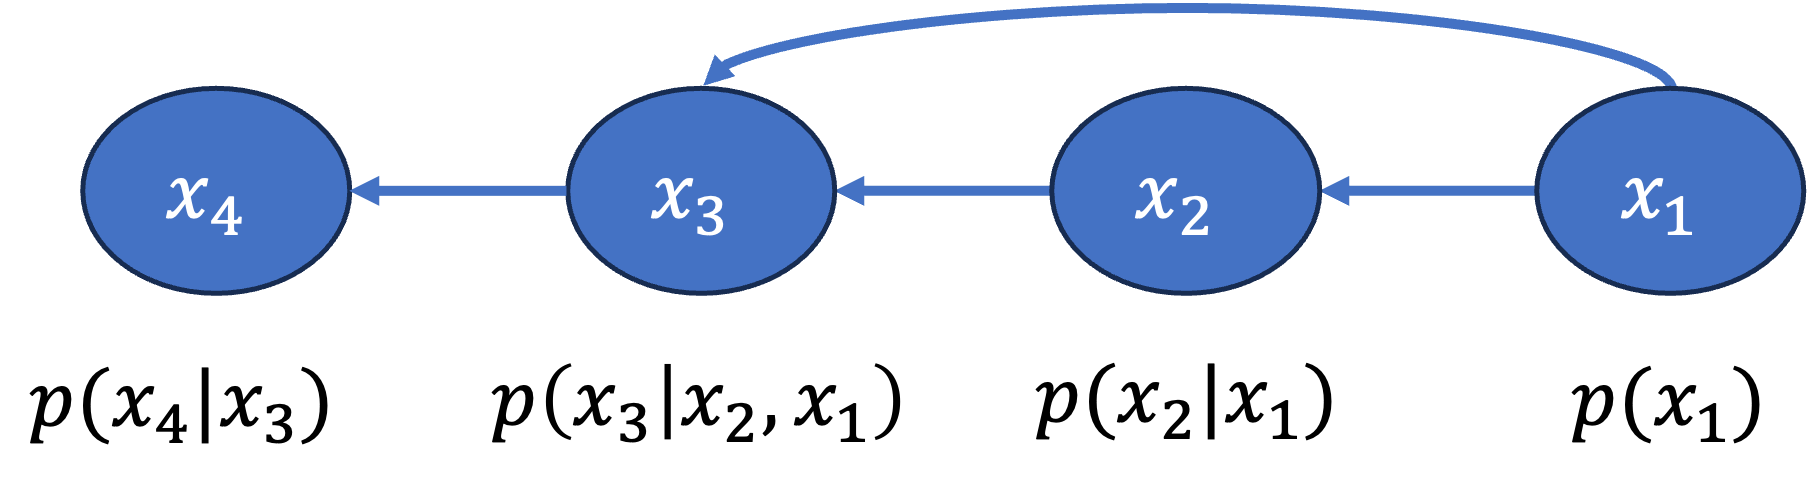
\includegraphics[width = 10cm, height = 3cm] {graph_vis.png}
\end{center}

\section{Bayesian Networks}

\begin{itemize}
    \item Factorization Definition (Chain rule for Bayesian Networks)\\
    The distribution P factorizes according to the DAG G, if
    \begin{center}
        $P(X_{1}, \ldots, X_{n}) = \prod_{i=1}^{n}P(X_{i} \mid Pax_{i}^{G})$
    \end{center}
    \item Bayesian Networks Definition \\
    Given the random variables V = ${X_{1}, X_{2}, \ldots, X_{n}}$, a Bayesian Network(BN) is a pair $B = (G; P_{B})$, where
    \begin{itemize}
        \item G is directed acyclic graph \textbf{(BN structure)} with node set V.
        \item $P_{B}$ is a probability function that factorizes according to G and is specified as a set of conditional probability distributions (CPDs) $P_{B}(X_{i} \mid Pax_{i})$ for all $X_{i} \in V$ \textbf{(BN parameters)}.
    \end{itemize}
\end{itemize}

\section{Covid Example}

\begin{itemize}
    \item Assume following joint probability distribution for Mask, Social distancing, Covid, Fever, Difficulty Breathing, and Ventilation
    \begin{center}
        $P(M,D,C,B,F,V) = P(F \mid C)P(V \mid B)P(B \mid C)P(C \mid M,D)P(M)P(D)$
    \end{center}
    \item Corresponding Bayesian Networks
    \begin{center}
        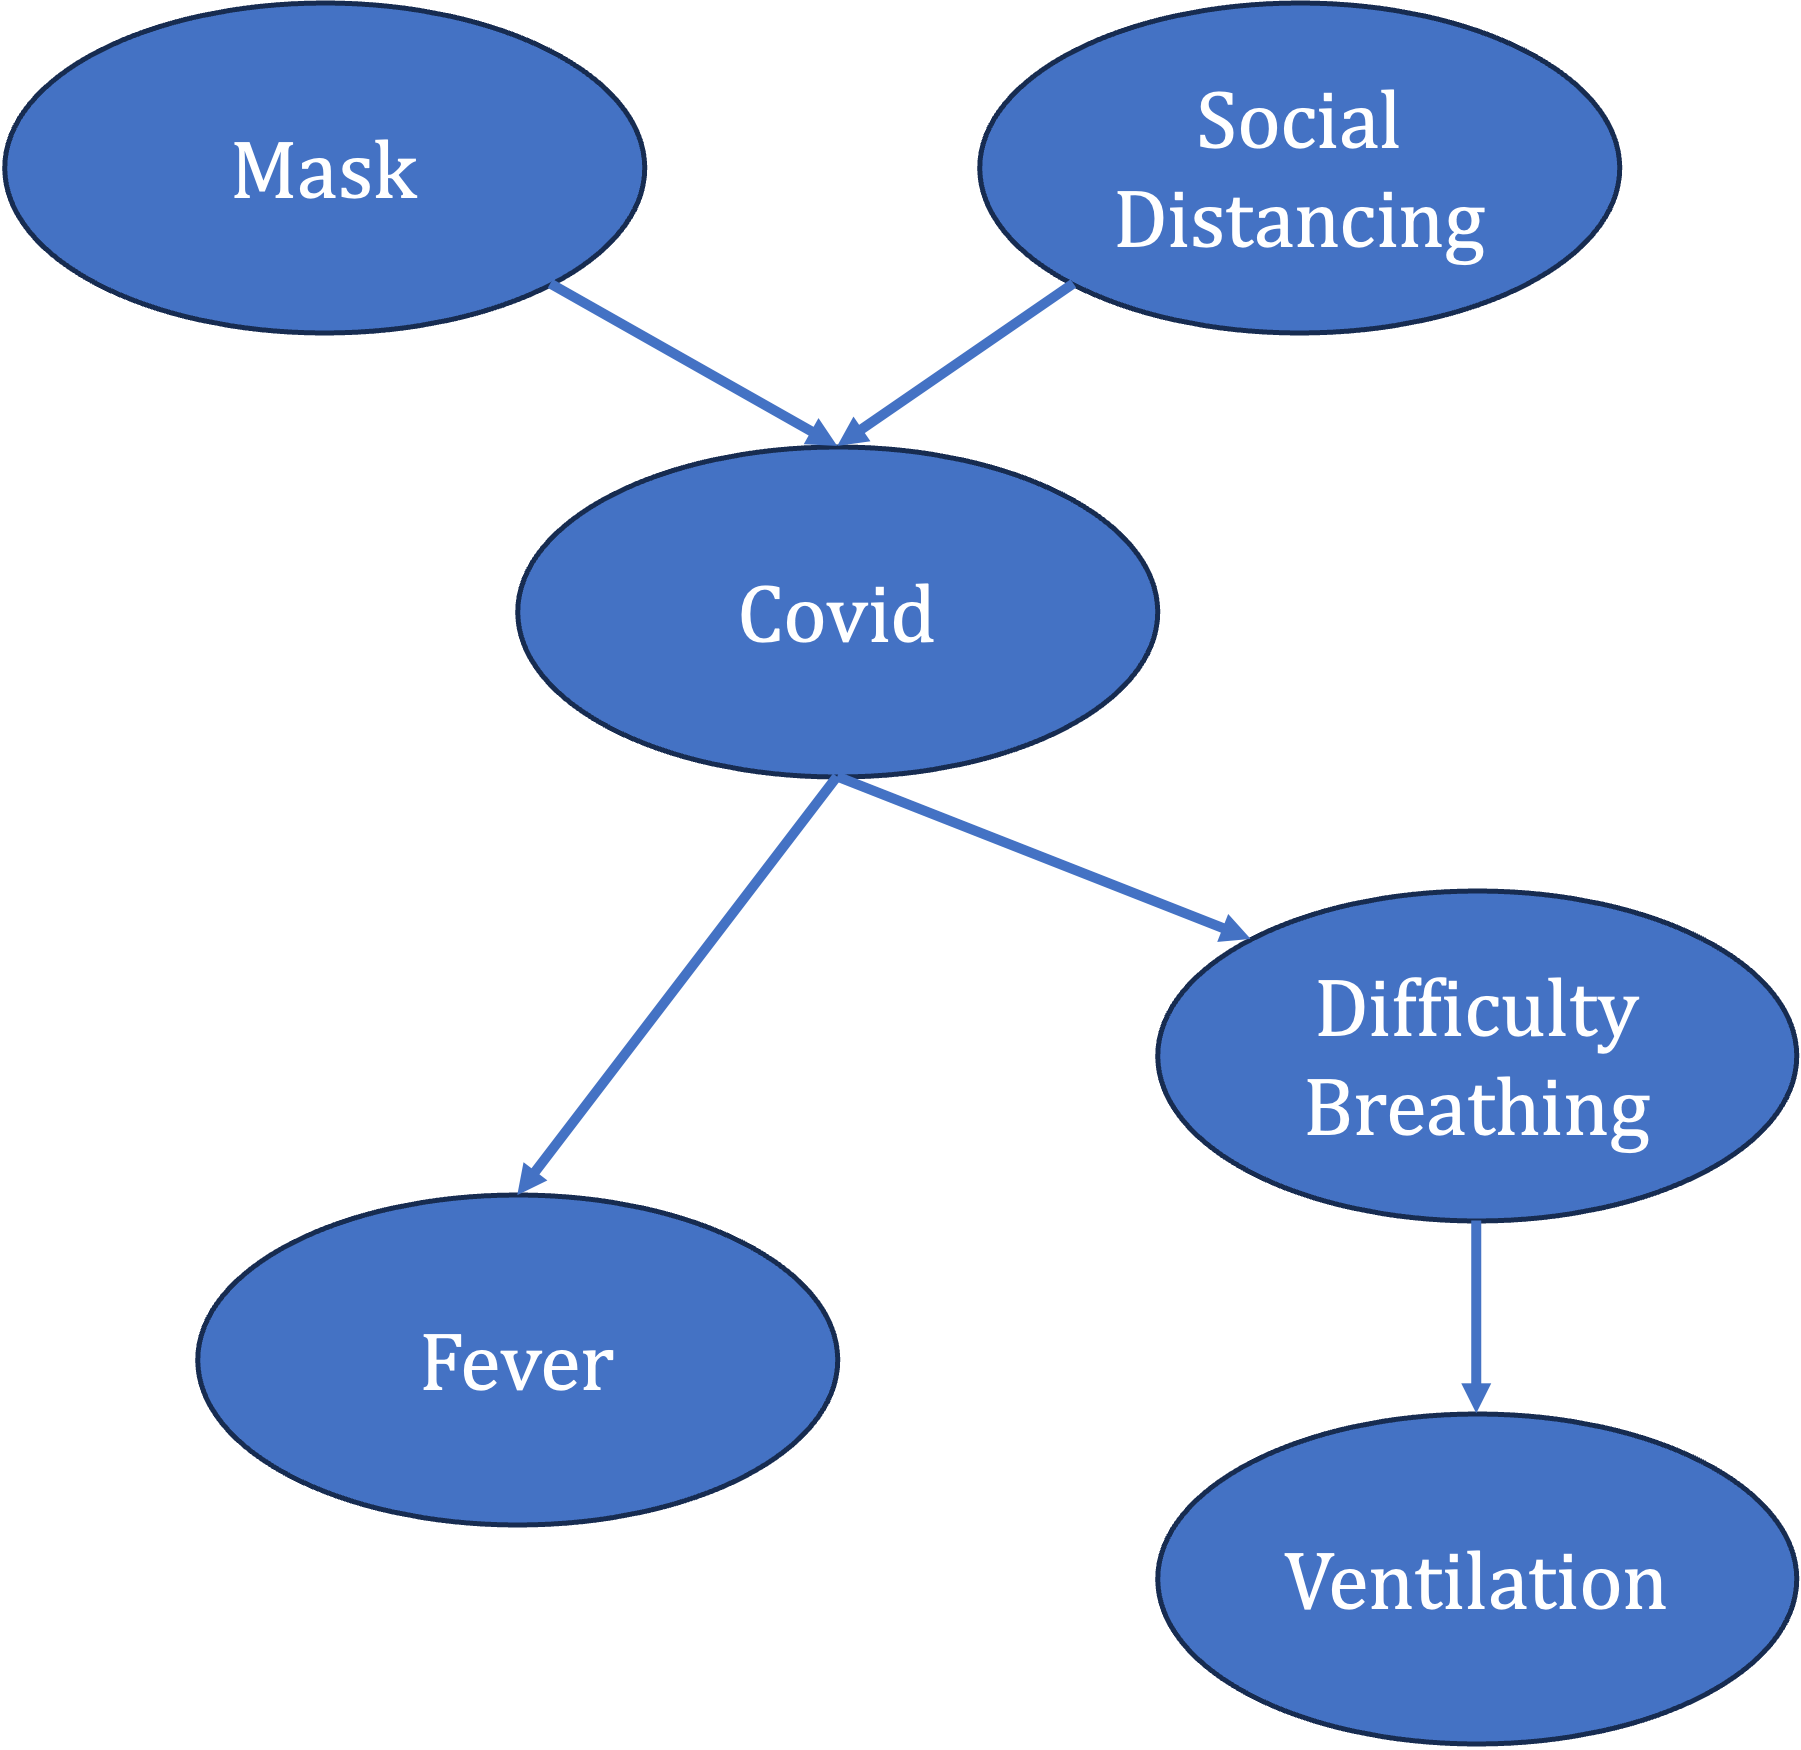
\includegraphics[width = 8cm, height = 7cm]{covid_graph.png}
    \end{center}
    BN structure is a representation of how the joint probability distribution of a set of random variables can be factorized.
\end{itemize}

\section{Summary: What is the Goal?}

The goal is to find from data, the correct factorization of the joint probability distribution. 

\begin{itemize}
    \item First, finding the conditional independence I(P).
    \item Use graphical visualization (BN), then determine which graph is the correct factorization.
\end{itemize}

%%------------------------------- chapter ------------------------------------

\chapter{From Factorization to Independence: I-map}

\section{Local Independence from BN}

\begin{itemize}
    \item The algebraic way of finding independence from factorization is complicated. The easier way is to use Bayesian Networks.

Assume we have the following factorization

\begin{center}
    $P(X_{1}, X_{2}, X_{3}, X_{4}) = P(X_{2} \mid X_{4})P(X_{4} \mid X_{}1)P(X_{1} \mid X_{3})P(X_{3})$ 
\end{center}

Equivalent BN

\begin{center}
    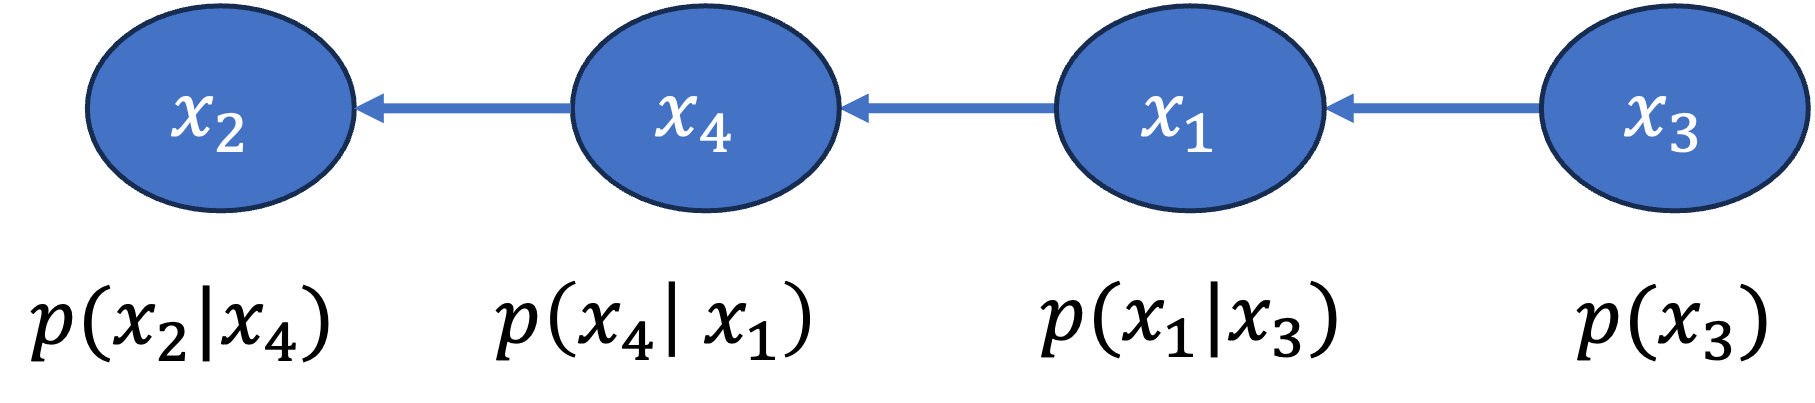
\includegraphics[width = 10cm, height = 2cm]{factor_ind.png}

    Then,
    $(X_{2} \perp X_{1}, X_{3} \mid X_{4}), (X_{4} \perp X_{3} \mid X_{1}) \in I(P)$ \\
    \vspace{0.3cm}
    Lack of edges indicates conditional independence. \\
    \vspace{0.3cm}
    $ (X_{2} \perp NonDescendents_{X_{2}} \mid Pax_{2}), (X_{4} \perp NonDescendents_{X_{4}} \mid Pax_{4}) \in I(P)$ \\
    $NonDescendents_{X_{i}}$ are all the nodes excluding the descendants of $X_{i}$.\\
    \vspace{0.3cm}
    These conditional independencies are known as the local independencies of the graph because they are conditioned on $X_{i}$'s parents.
\end{center}

\item Local Independence Definition

Given the graph G, the set of \textbf{local (Markov) independencies}, denoted by $I_{l}(G)$, consists of

\begin{center}
    $(X_{i} \perp NonDescendents_{X_{i}} \mid Pax_{i}^{G})\ \forall i$
\end{center}

\item Independence-map (I\_map) Definition

\begin{center}
    G is an I\_map for P if $I_{l}^{G} \subseteq I(P)$
\end{center}

So, G being an I\_map for P means that P satisfies the local independencies of G.

\item I\_map Theorem\\
Let G be a DAG and P be an joint distribution over a set of random variables. P factorizes according to G, if and only if G is a I\_map for P.

\end{itemize}

\section{$I_{l}(G)\ and\ I(P)$: Example}

\begin{itemize}
    \item Consider the joint distribution P over $X_{1}, X_{2}, \ldots, X_{4}$, where
    \begin{center}
        I(P) =  {$(X_{4} \perp X_{2}, X_{1} \mid X_{3})$ and its derivations}
    \end{center}
    \begin{itemize}
        \item Factorization 1
        \begin{itemize}
            \item Does P satisfy the following factorization?
        \begin{center}
            $P(X_{1}, \ldots, X_{4}) = P(X_{4} \mid X_{3})P(X_{3} \mid X_{2},X_{1})P(X_{2} \mid X_{1})P(X_{1})$ 
        \end{center}
        \item Equivalent graph G
        \begin{center}
            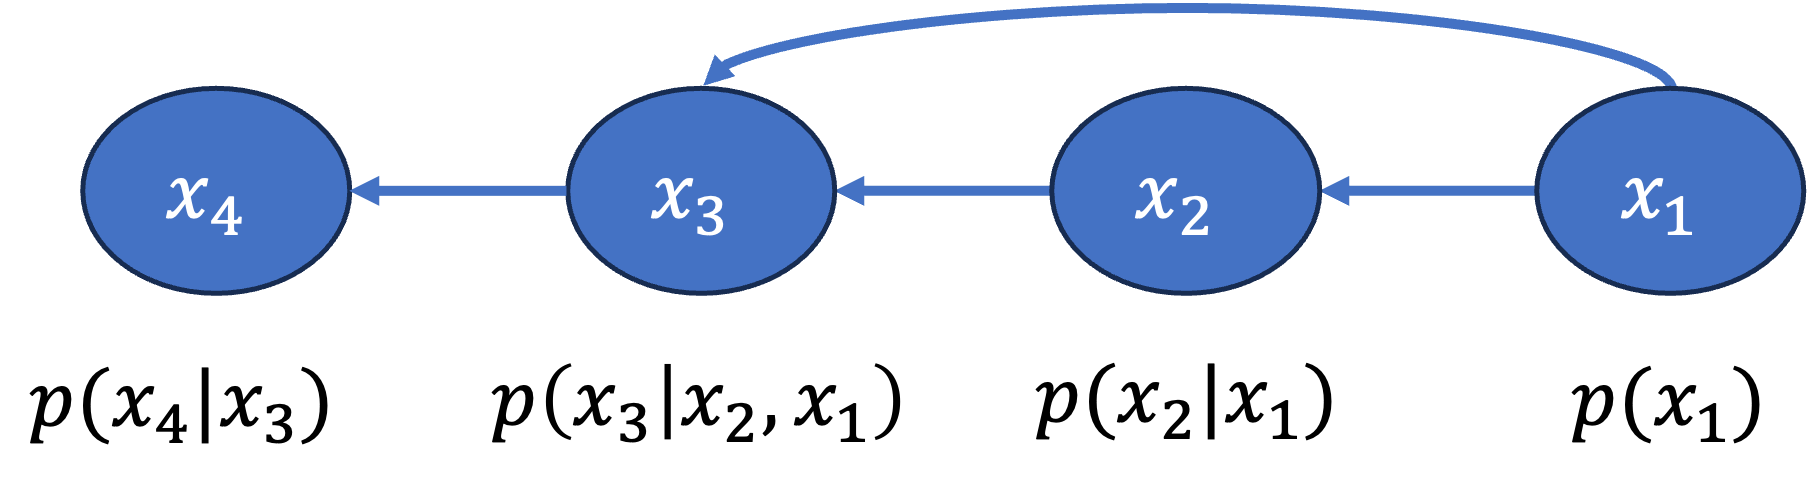
\includegraphics[width = 10cm, height = 3cm]{graph_vis.png}\\
            imposing local independencies:\\
            $I_{l}(G) = {(X_{4} \perp X_{2}, X_{1} \perp X_{3})}$\\
            Therefore, $I_{l}(G) \subseteq I(P)$, G is an i-map for P.
        \end{center}
        \end{itemize}
        \item Factorization 2
        \begin{itemize}
            \item Does P satisfy the following factorization?
        \begin{center}
            $P(X_{1}, \ldots, X_{4}) = P(X_{4} \mid X_{3}, X_{2},X_{1})P(X_{3} \mid X_{2},X_{1})P(X_{2} \mid X_{1})P(X_{1})$ 
        \end{center}
        \item Equivalent graph G
        \begin{center}
            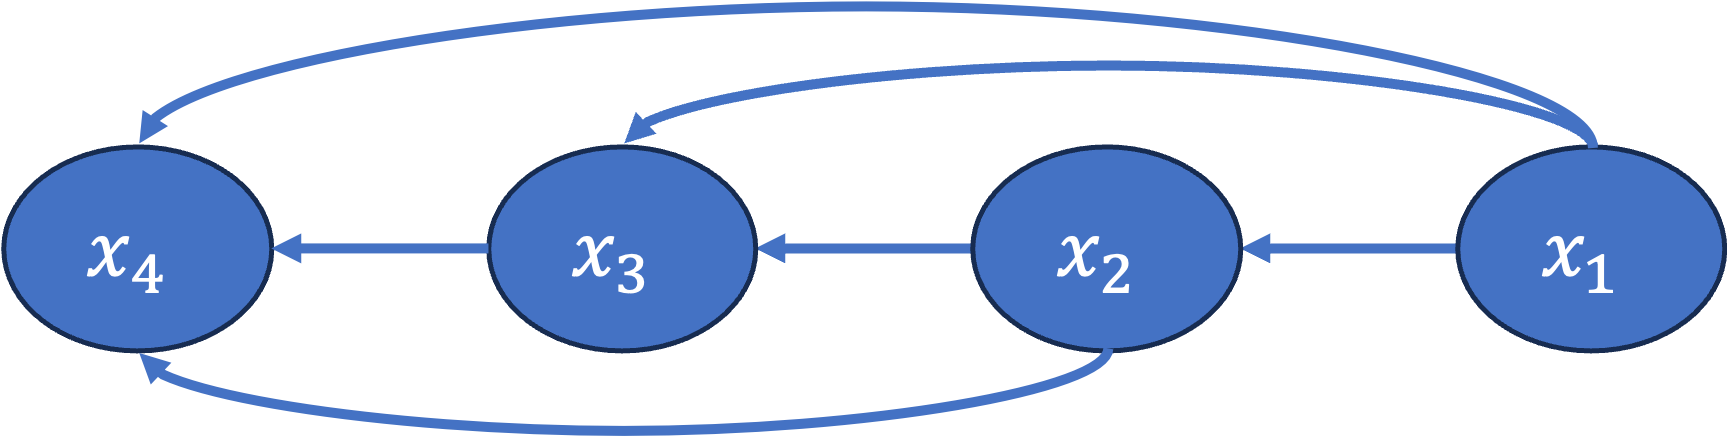
\includegraphics[width = 10cm, height = 3cm]{graph_vis2.png}\\
            imposing local independencies:\\
            $I_{l}(G) = \emptyset $\\
            Therefore, $I_{l}(G) \subseteq I(P)$, G is an i-map for P.
        \end{center}
        \end{itemize}
        \item There could be more than one i\_map for P.
\end{itemize}

\end{itemize}

\section{Summary: What is the Goal?}

The goal is to find from data, the correct factorization of the joint probability distribution. 

\begin{itemize}
    \item First, finding the conditional independence I(P)
    \item For each factorization, we could draw a bayesian nets, and we could write down local independencies $I_{l}^{G}$. If $I_{l}^{G} \subseteq I(P)$, then G is i\_map for P
    \item There could be several i\_map for P, the problem now is which one to choose?
\end{itemize}

%%------------------------------- chapter ------------------------------------
\chapter{Minimal I-map}

\section{Multiple I-map}

\begin{itemize}
    \item Consider the joint distribution P over $X_{1}, X_{2}, \ldots, X_{4}$, where
    \begin{center}
        I(P) =  {$(X_{4} \perp X_{2}, X_{1} \mid X_{3})$ and its derivations}
    \end{center}
    \begin{itemize}
        \item Graph1
        
        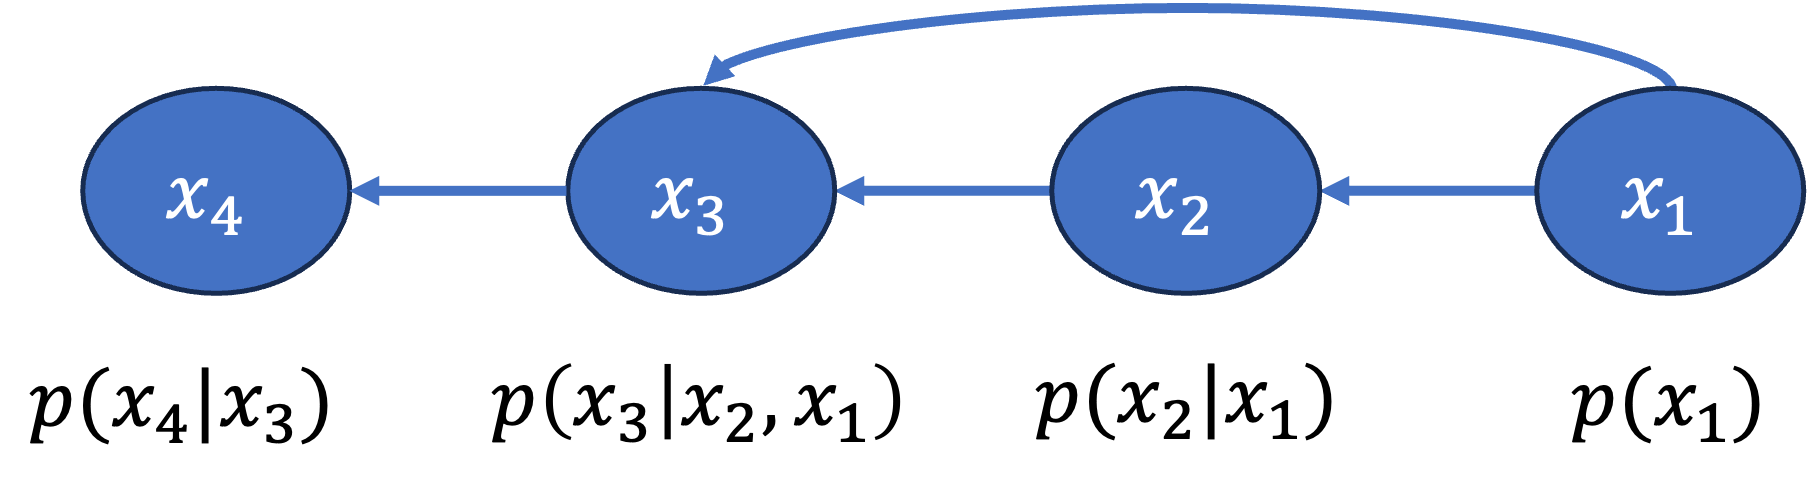
\includegraphics[width = 10cm, height = 3cm]{graph_vis.png}\\
        $I_{l}(G_{1}) = {(X_{4} \perp X_{2}, X_{1} \perp X_{3})}$\\
        Therefore, $I_{l}(G_{1}) \subseteq I(P)$, $G_{1}$ is an i-map for P.

        \item Graph2
        
        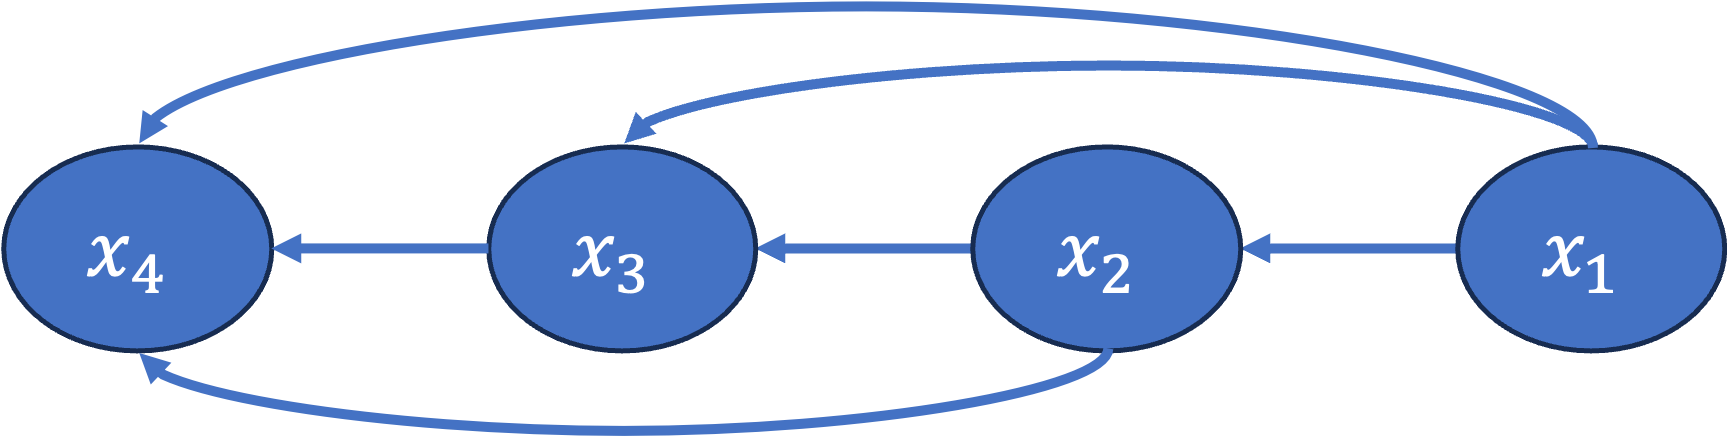
\includegraphics[width = 10cm, height = 3cm]{graph_vis2.png}\\
        $I_{l}(G_{2}) = \emptyset $\\
        Therefore, $I_{l}(G_{2}) \subseteq I(P)$, $G_{2}$ is an i-map for P.

        \item Graph3
        
        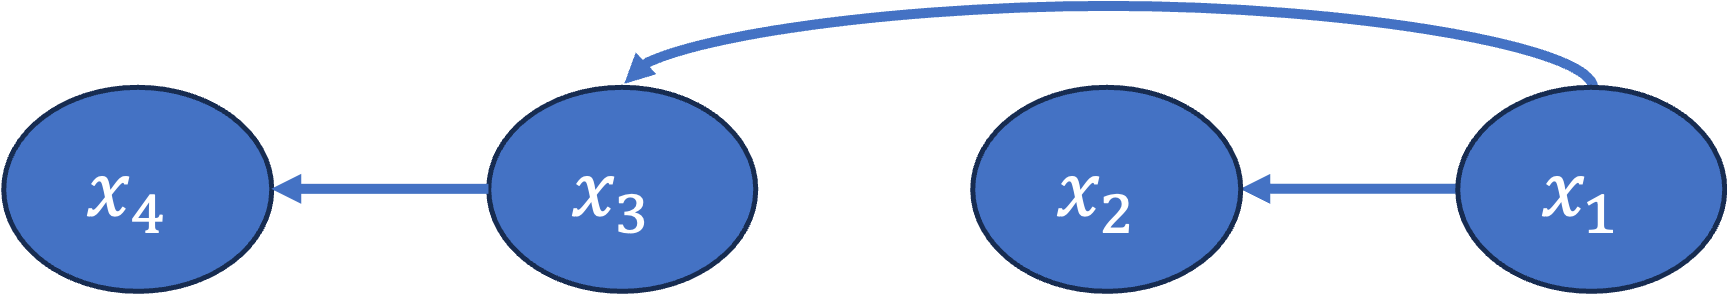
\includegraphics[width = 10cm, height = 2cm]{imap_1.png}\\
        $(X_{3} \perp X_{2} \mid X_{1}) \in I_{l}(G_{3})$
        $(X_{3} \perp X_{2} \mid X_{1}) \notin I(P)$
        Therefore, $G_{3}$ is not an imap for p.
\end{itemize}

\section{Minimal I-map}
\begin{itemize}
    \item Definition
    
    A graph G is a minimal I-map for P if it is an I-map for P, and if the removal of any edge from G makes it not an I-map.

    \item Minimal I-maps are not Unique
    
    \begin{itemize}
        \item $G_{1}$ is a minimal I-map
        
        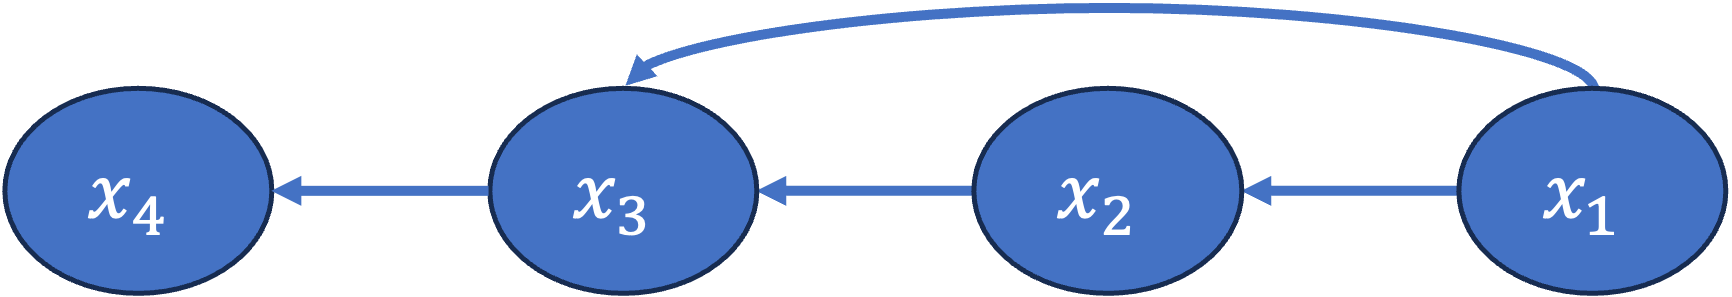
\includegraphics[width = 10cm, height = 2cm]{imap_2.png}
        \item By simply reversing one edge, $G_{2}$ is also a minimal I-map.
        
        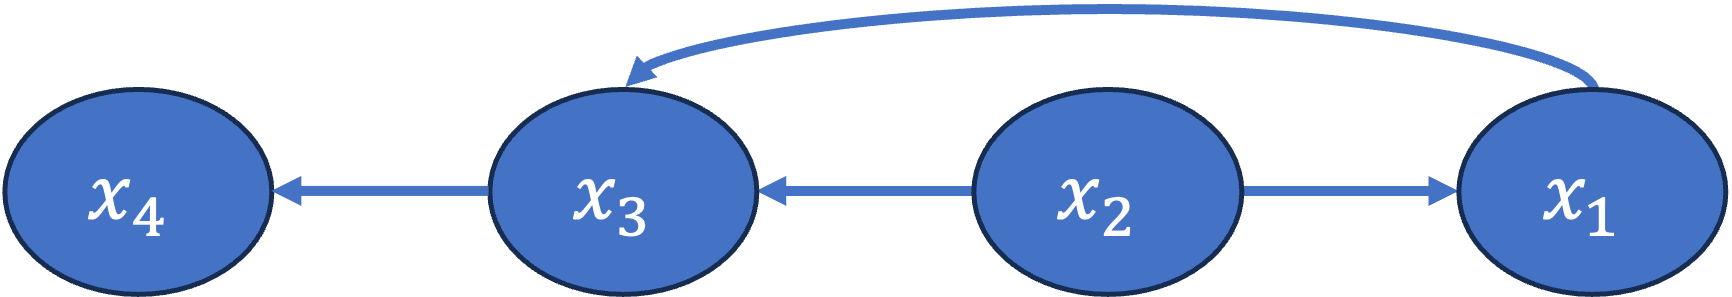
\includegraphics[width = 10cm, height = 2cm]{imap_3.png}
    \end{itemize}
\end{itemize}
\end{itemize}

\section{Summary: What is the Goal?}

The goal is to find from data, the correct factorization of the joint probability distribution. 

\begin{itemize}
    \item First, finding the conditional independence I(P)
    \item For each factorization, we could draw a bayesian nets, and we could write down local independencies $I_{l}^{G}$. If $I_{l}^{G} \subseteq I(P)$, then G is i\_map for P
    \item There could be several i\_map for P, the problem now is which one to choose? The minimal I-maps.
\end{itemize}

%%------------------------------- chapter ------------------------------------

\chapter{Global Independence}

\section{Global Conditional Independence}

\begin{itemize}
    \item Consider the joint distribution P over $X_{1}, X_{2}, \ldots, X_{4}$, factorizing as
    \begin{center}
        $P(X_{1}, \ldots, X_{4}) = P(X_{4} \mid X_{3}) P(X_{3} \mid X_{2}) P(X_{2} \mid X_{1})P(X_{1})$\\
        \vspace{0.5cm}
        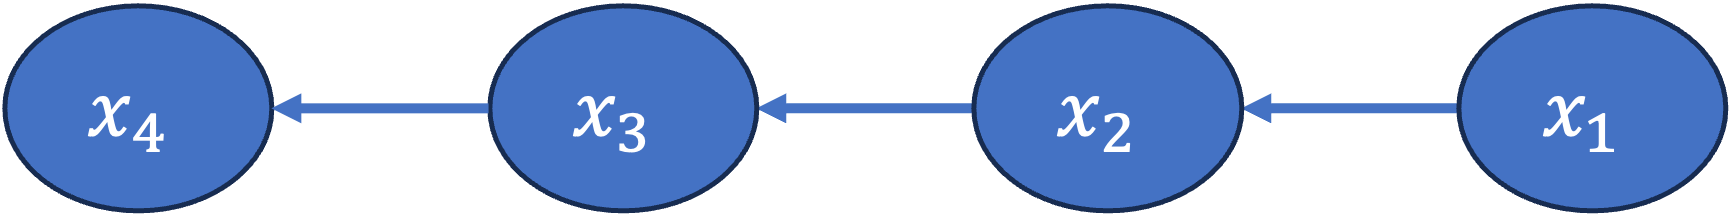
\includegraphics{global_indep1.png}\\
        \vspace{0.5cm}
        Equivalent graph G, imposing the local indepencies:\\
        \vspace{0.5cm}
        $I_{l}(G) = {(X_{4} \perp X_{1}, X_{2} \mid X_{3}), (X_{3} \perp X_{1} \mid X_{2})}$
    \end{center}
    \item What if we condition $X_{4}$ on $X_{2}$
    \begin{center}
    \begin{equation}
    \begin{split}
        P(X_{4},X_{1} \mid X_{2}) & = \frac{P(X_{4},X_{1},X_{2})}{P(X_{2})}\\
        & = \frac{\sum_{X_{3}}P(X_{4},X_{3},X_{2},X_{1})}{P(X_{2})} \\
        & = \frac{\sum_{X_{3}}P(X_{4} \mid X_{3})P(X_{3} \mid X_{2})P(X_{2} \mid X_{1})P(X_{1})}{P(X_{2})} \\
        & = \frac{\sum_{X_{3}}P(X_{4} \mid X_{3})P(X_{3} \mid X_{2})P(X_{2})P(X_{1} \mid X_{2})}{P(X_{2})} \\
        & = \frac{\sum_{X_{3}}P(X_{4},X_{3},X_{2})P(X_{1} \mid X_{2})}{P(X_{2})} \\
        & = \frac{P(X_{4},X_{2})P(X_{1} \mid X_{2})}{P(X_{2})} \\
        & = P(X_{4} \mid X_{2})P(X_{1} \mid X_{2}) \\
    \end{split}
    \end{equation}
    \end{center}
    \item This type of conditional independence holds for a general graph including node $V_{1}$ and $V_{2}$ that are connected by some path, but become disconnected if node Z is removed.
    \begin{center}
        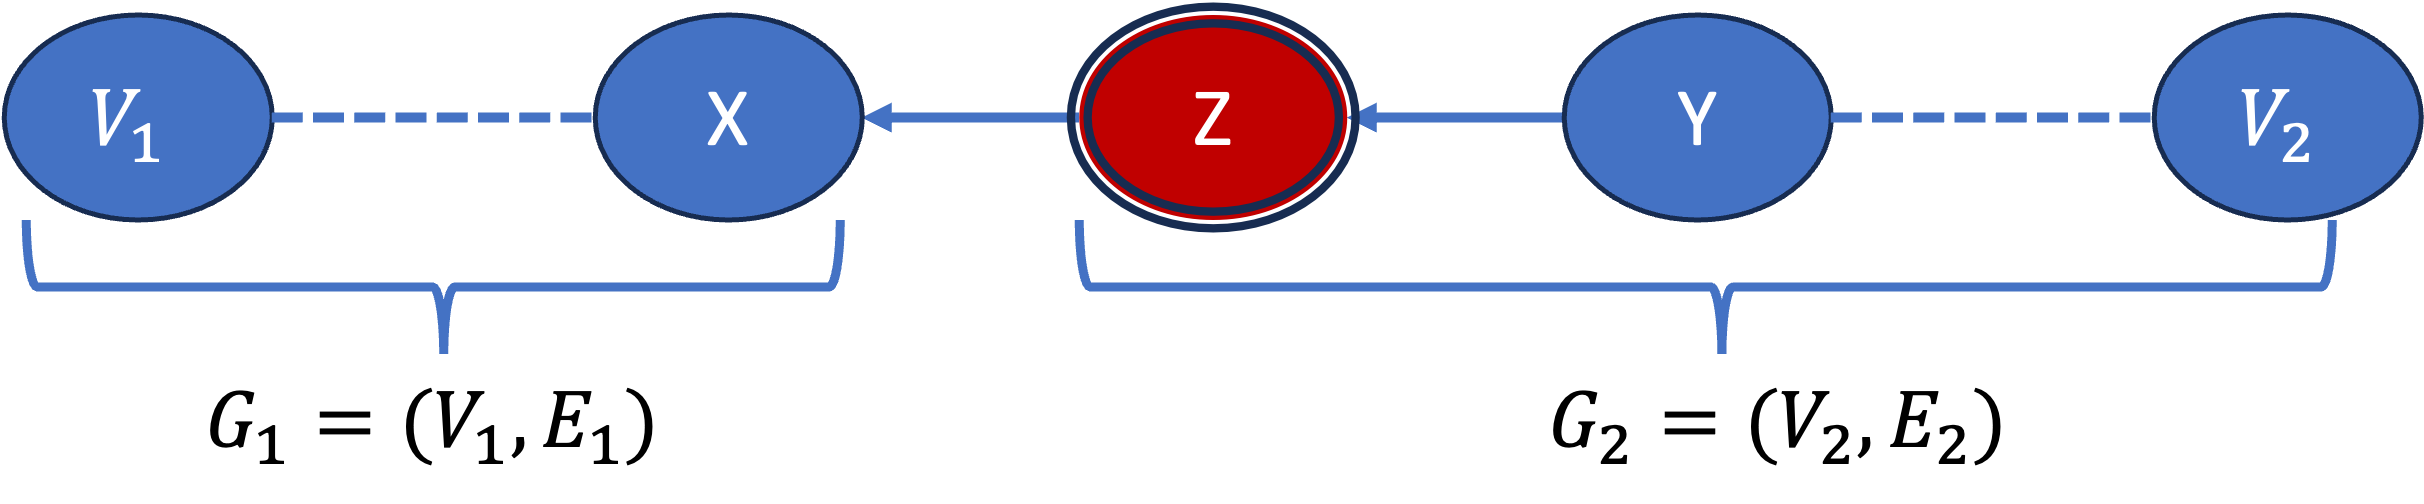
\includegraphics[width = 15cm, height = 3cm]{global_indep2.png}\\
        \vspace{0.5cm}
        Hence, $V_{1} \perp V_{2} \mid Z$ \\
        \vspace{0.5cm}
        It holds true for the following graphs:\\
        \vspace{0.5cm}
        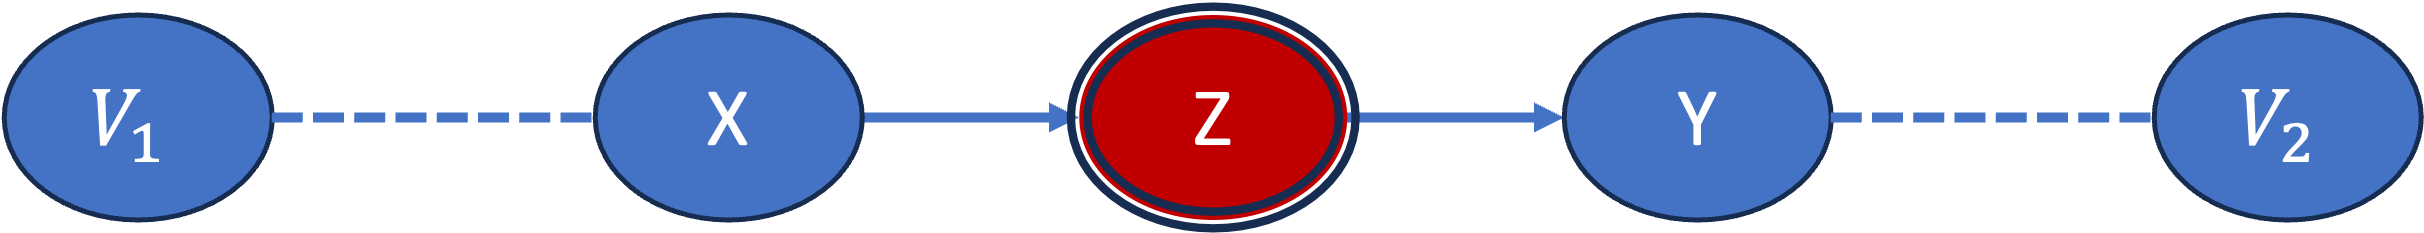
\includegraphics[width = 12cm, height = 1cm]{global_indep3.png}\\
        \vspace{0.5cm}
        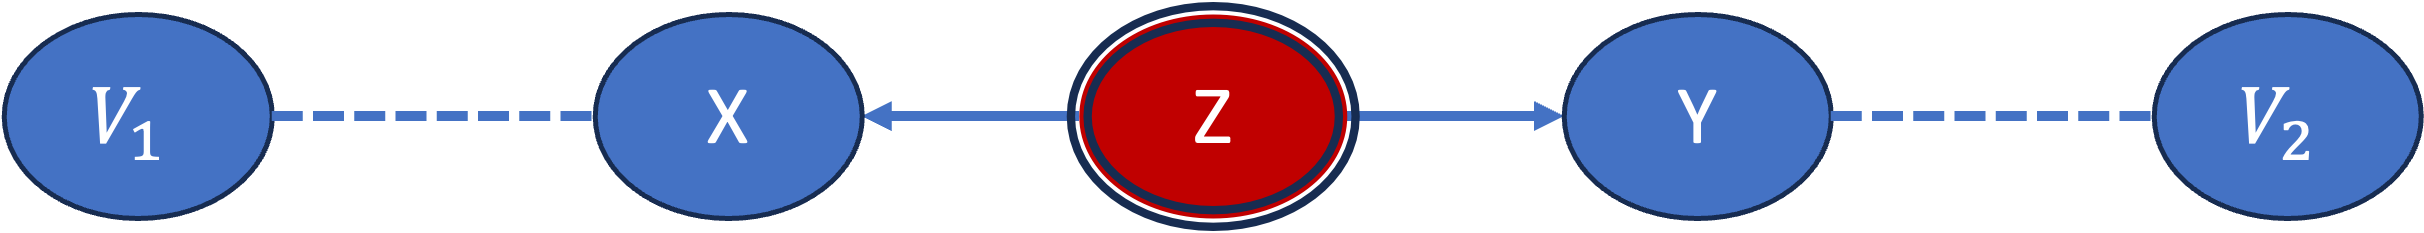
\includegraphics[width = 12cm, height = 1cm]{global_indep4.png}\\
        The observed node Z blocks information flows between X and Y, and consequently $V_{1}$ and $V_{2}$
    \end{center}

    \item What about X -> Z <- Y, known as the v-structure
    \begin{center}
        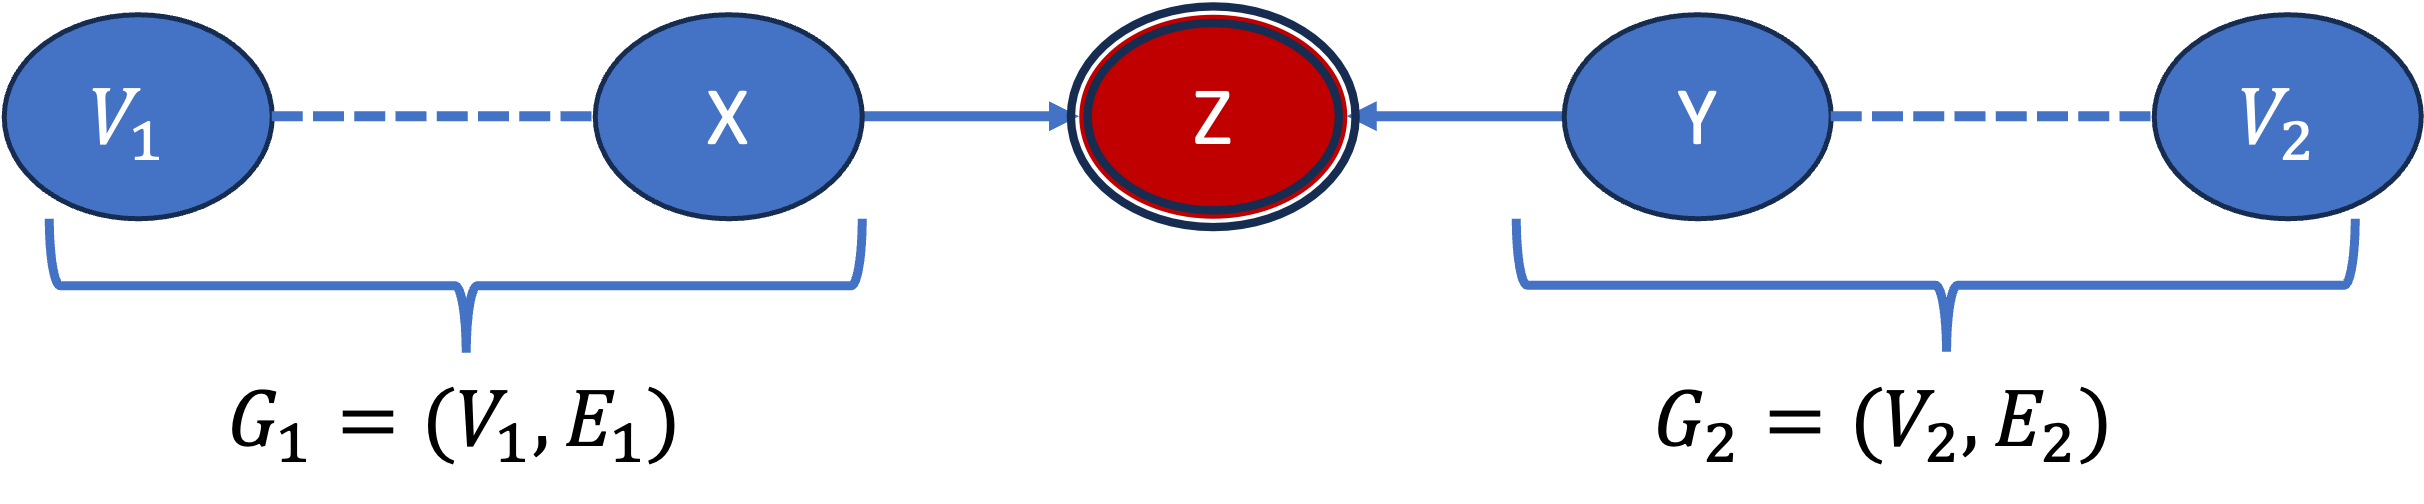
\includegraphics[width = 12cm, height = 3cm]{global_indep5.png}\\
    \end{center}
    \begin{equation}
    \begin{split}
        P(V_{1},V_{2}) & = \sum_{v \neq V_{1},V_{2}} \prod_{v}P(v \mid Pa_{v})\\
        & = \sum_{v \neq V_{1},V_{2}} \prod_{v \in V_{1}}P(v \mid Pa_{v}) \prod_{v \in V_{2}}P(v \mid Pa_{v})P(Z \mid X,Y)\\
        & = \sum_{v \neq V_{1},V_{2},Z} \prod_{v \in V_{1}}P(v \mid Pa_{v}) \prod_{v \in V_{2}}P(v \mid Pa_{v})\sum_{Z}P(Z \mid X,Y)\\
        & = \sum_{v \neq V_{1},V_{2},Z}P(V_{1})P(V_{2})\\
        & = P(V_{1})P(V_{2})\\
    \end{split}
    \end{equation}
    Hence, $V_{1} \perp V_{2}$ 
    \item The conclusion does not hold if Z had an observed descendant
    \begin{center}
        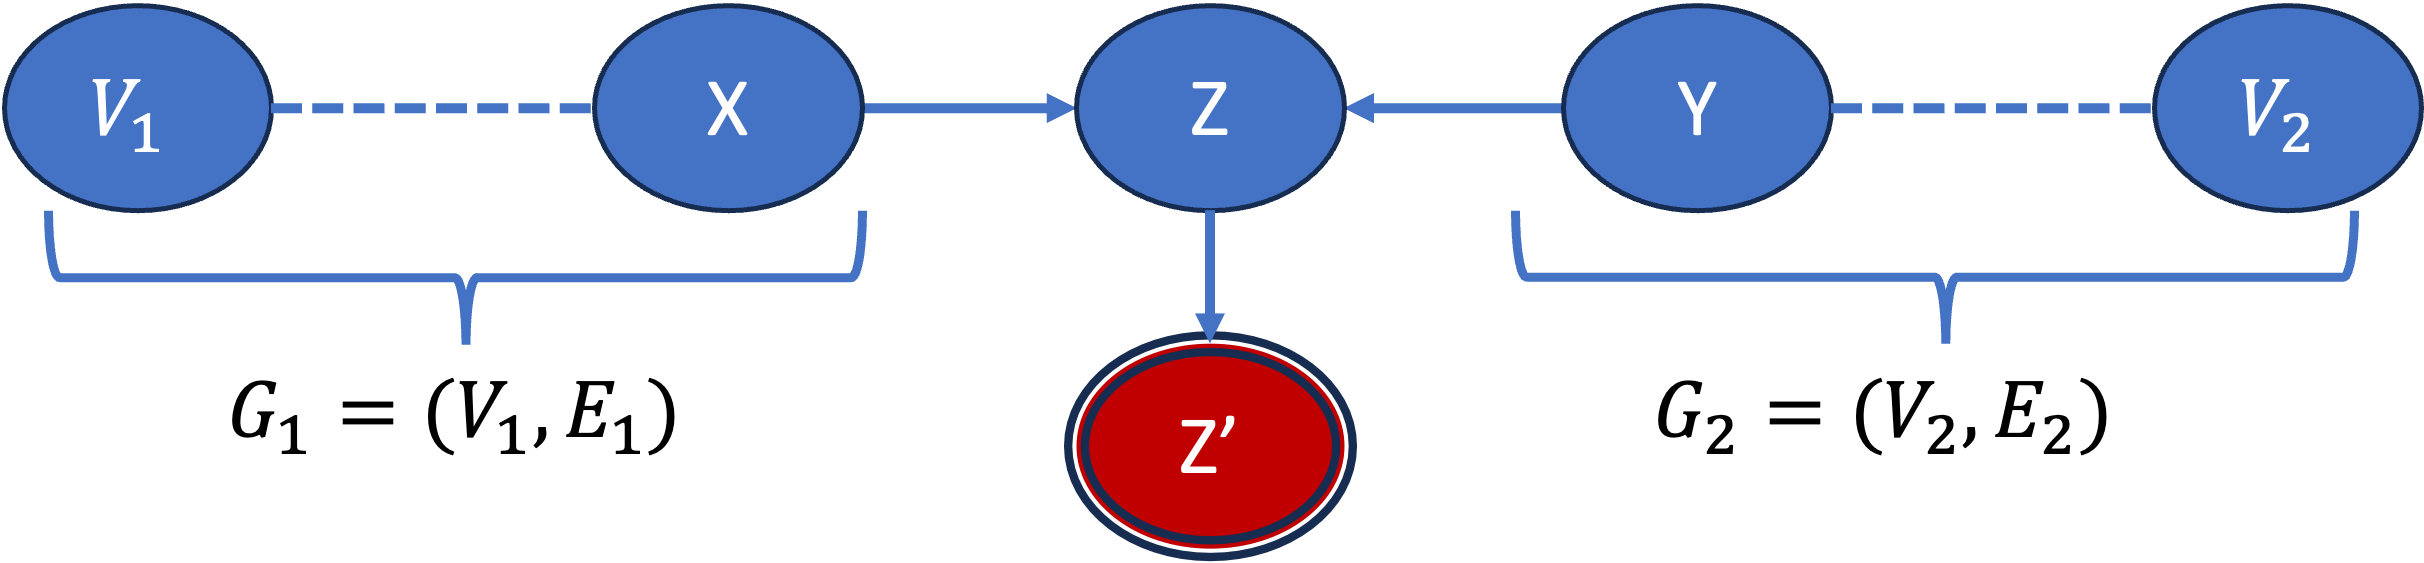
\includegraphics[width = 12cm, height = 3cm]{global_indep6.png}\\
    \end{center}
\end{itemize}

\section{Trails}

\begin{itemize}
    \item In all of the cases, there are two nodes, v1 and v2.
    \begin{itemize}
        \item information flows between them, they can be dependent.\\
        \vspace{0.5cm}
        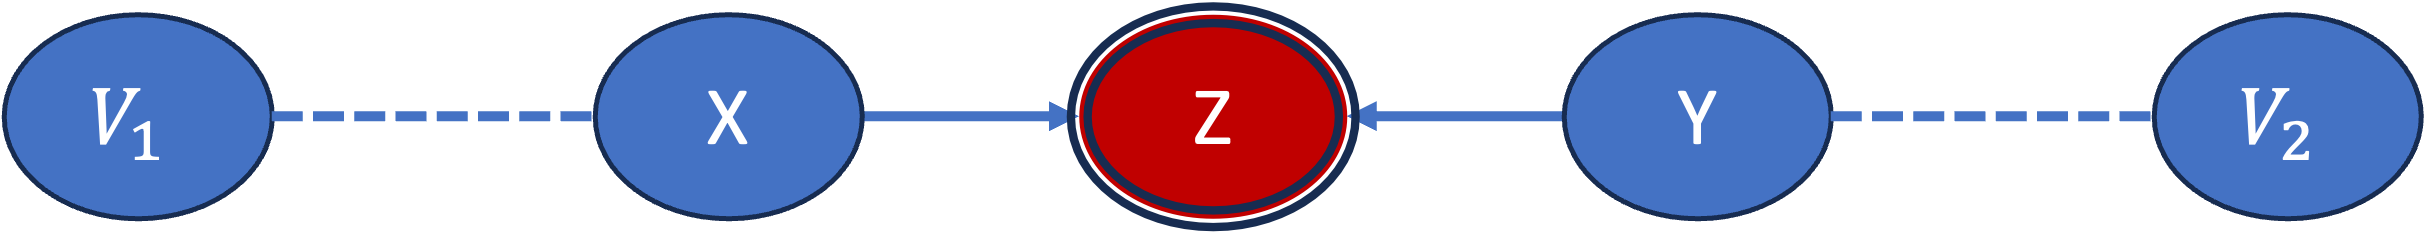
\includegraphics[width = 12cm, height = 1cm]{global_indep7.png}
        \item information flow if blocked, they aren globally conditionally independent.\\
        \vspace{0.5cm}
        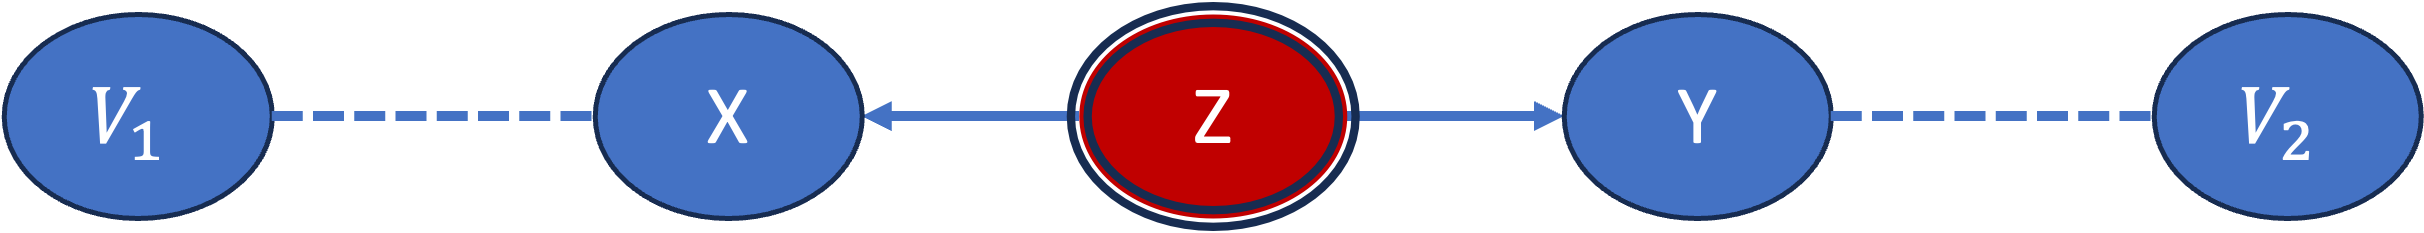
\includegraphics[width = 12cm, height = 1cm]{global_indep4.png}
    \end{itemize}
    \item A sequence of consecutively connected nodes x1 <=> x2 \ldots <=> xn in a graph is called a trail.
    \item A trail is \textbf{active} if information flows and \textbf{inactive} if the flow is blocked.
    \item Three types of inactive trails
    \begin{itemize}
        \item Indirect, causal effect\\
        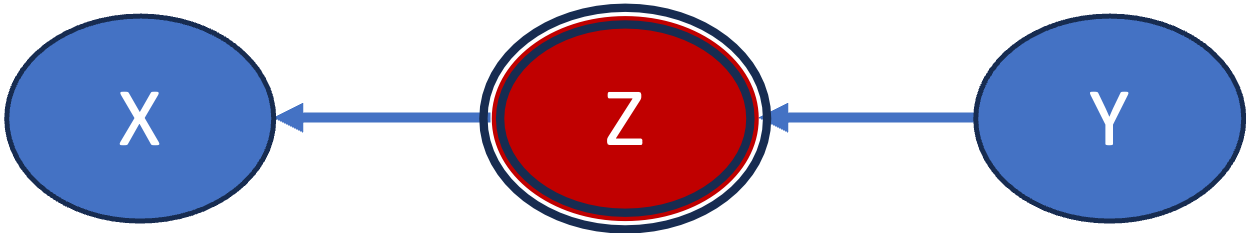
\includegraphics[width = 6cm, height = 1cm]{inactive_t1.png}
        \item Common cause\\
        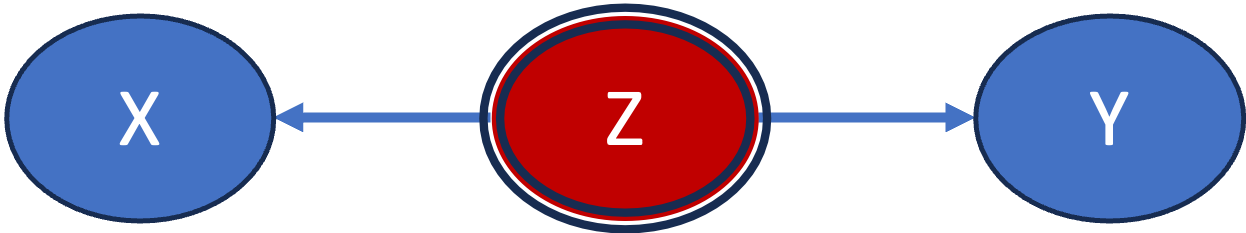
\includegraphics[width = 6cm, height = 1cm]{inactive_t2.png}
        \item V-structure\\
        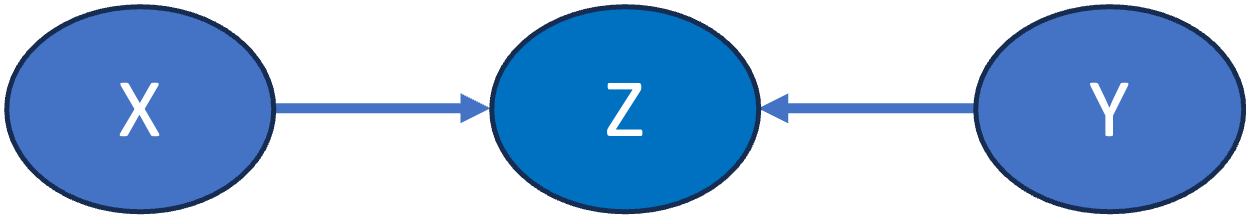
\includegraphics[width = 6cm, height = 1cm]{inactive_t3.png}
        \item Inactive trail <=> Global conditional independence
    \end{itemize}
    \item Four types of active trails
    \begin{itemize}
        \item Indirect, causal effect\\
        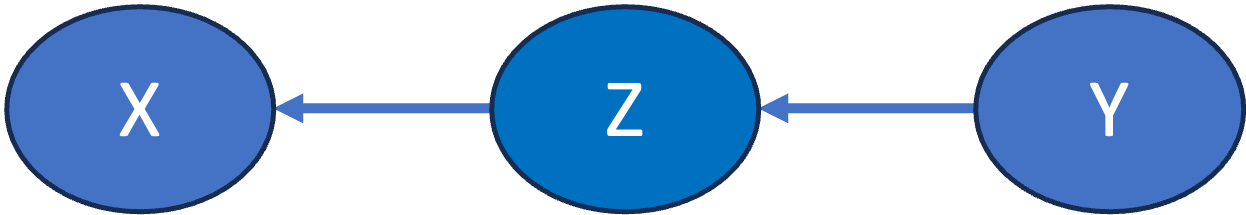
\includegraphics[width = 6cm, height = 1cm]{active_t1.png}
        \item Common cause\\
        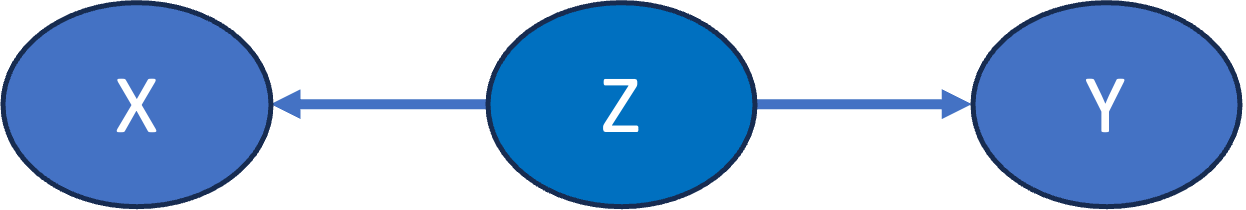
\includegraphics[width = 6cm, height = 1cm]{active_t2.png}
        \item V-structure\\
        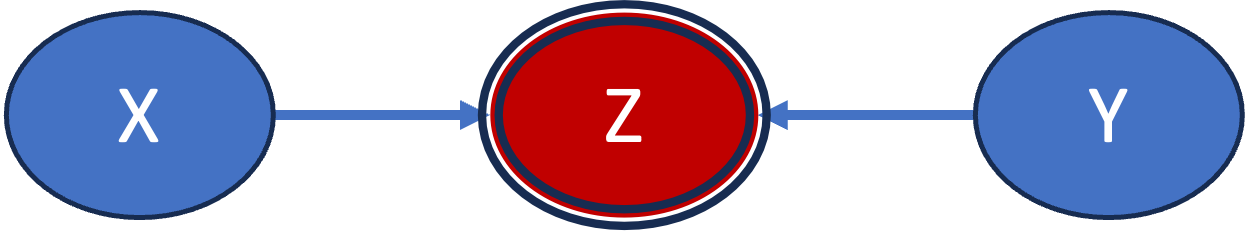
\includegraphics[width = 6cm, height = 1cm]{active_t3.png}
        \item V-structure\\
        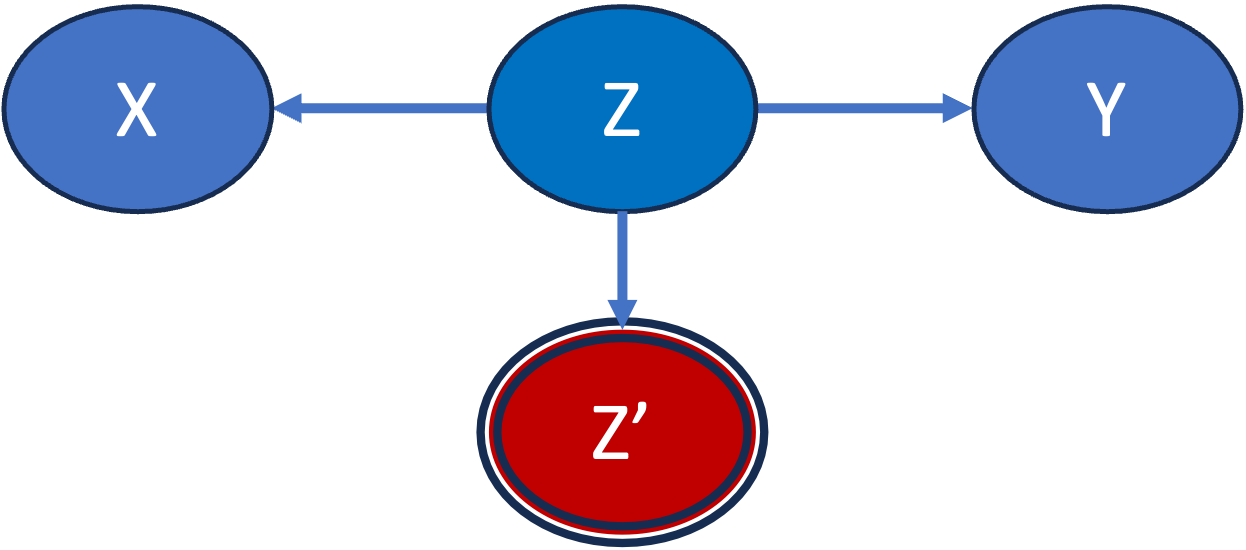
\includegraphics[width = 6cm, height = 3cm]{active_t4.png}
    \end{itemize}
    \item Common Cause Example: Consider the trail Fever <- Flu -> Cough in the covid example
    \begin{itemize}
        \item If $Z = \emptyset$ => active trail
        \begin{center}
        Fever and cough are dependent: a person with fever gives us information about that person having flu or coughing.
        \vspace{0.5cm}
        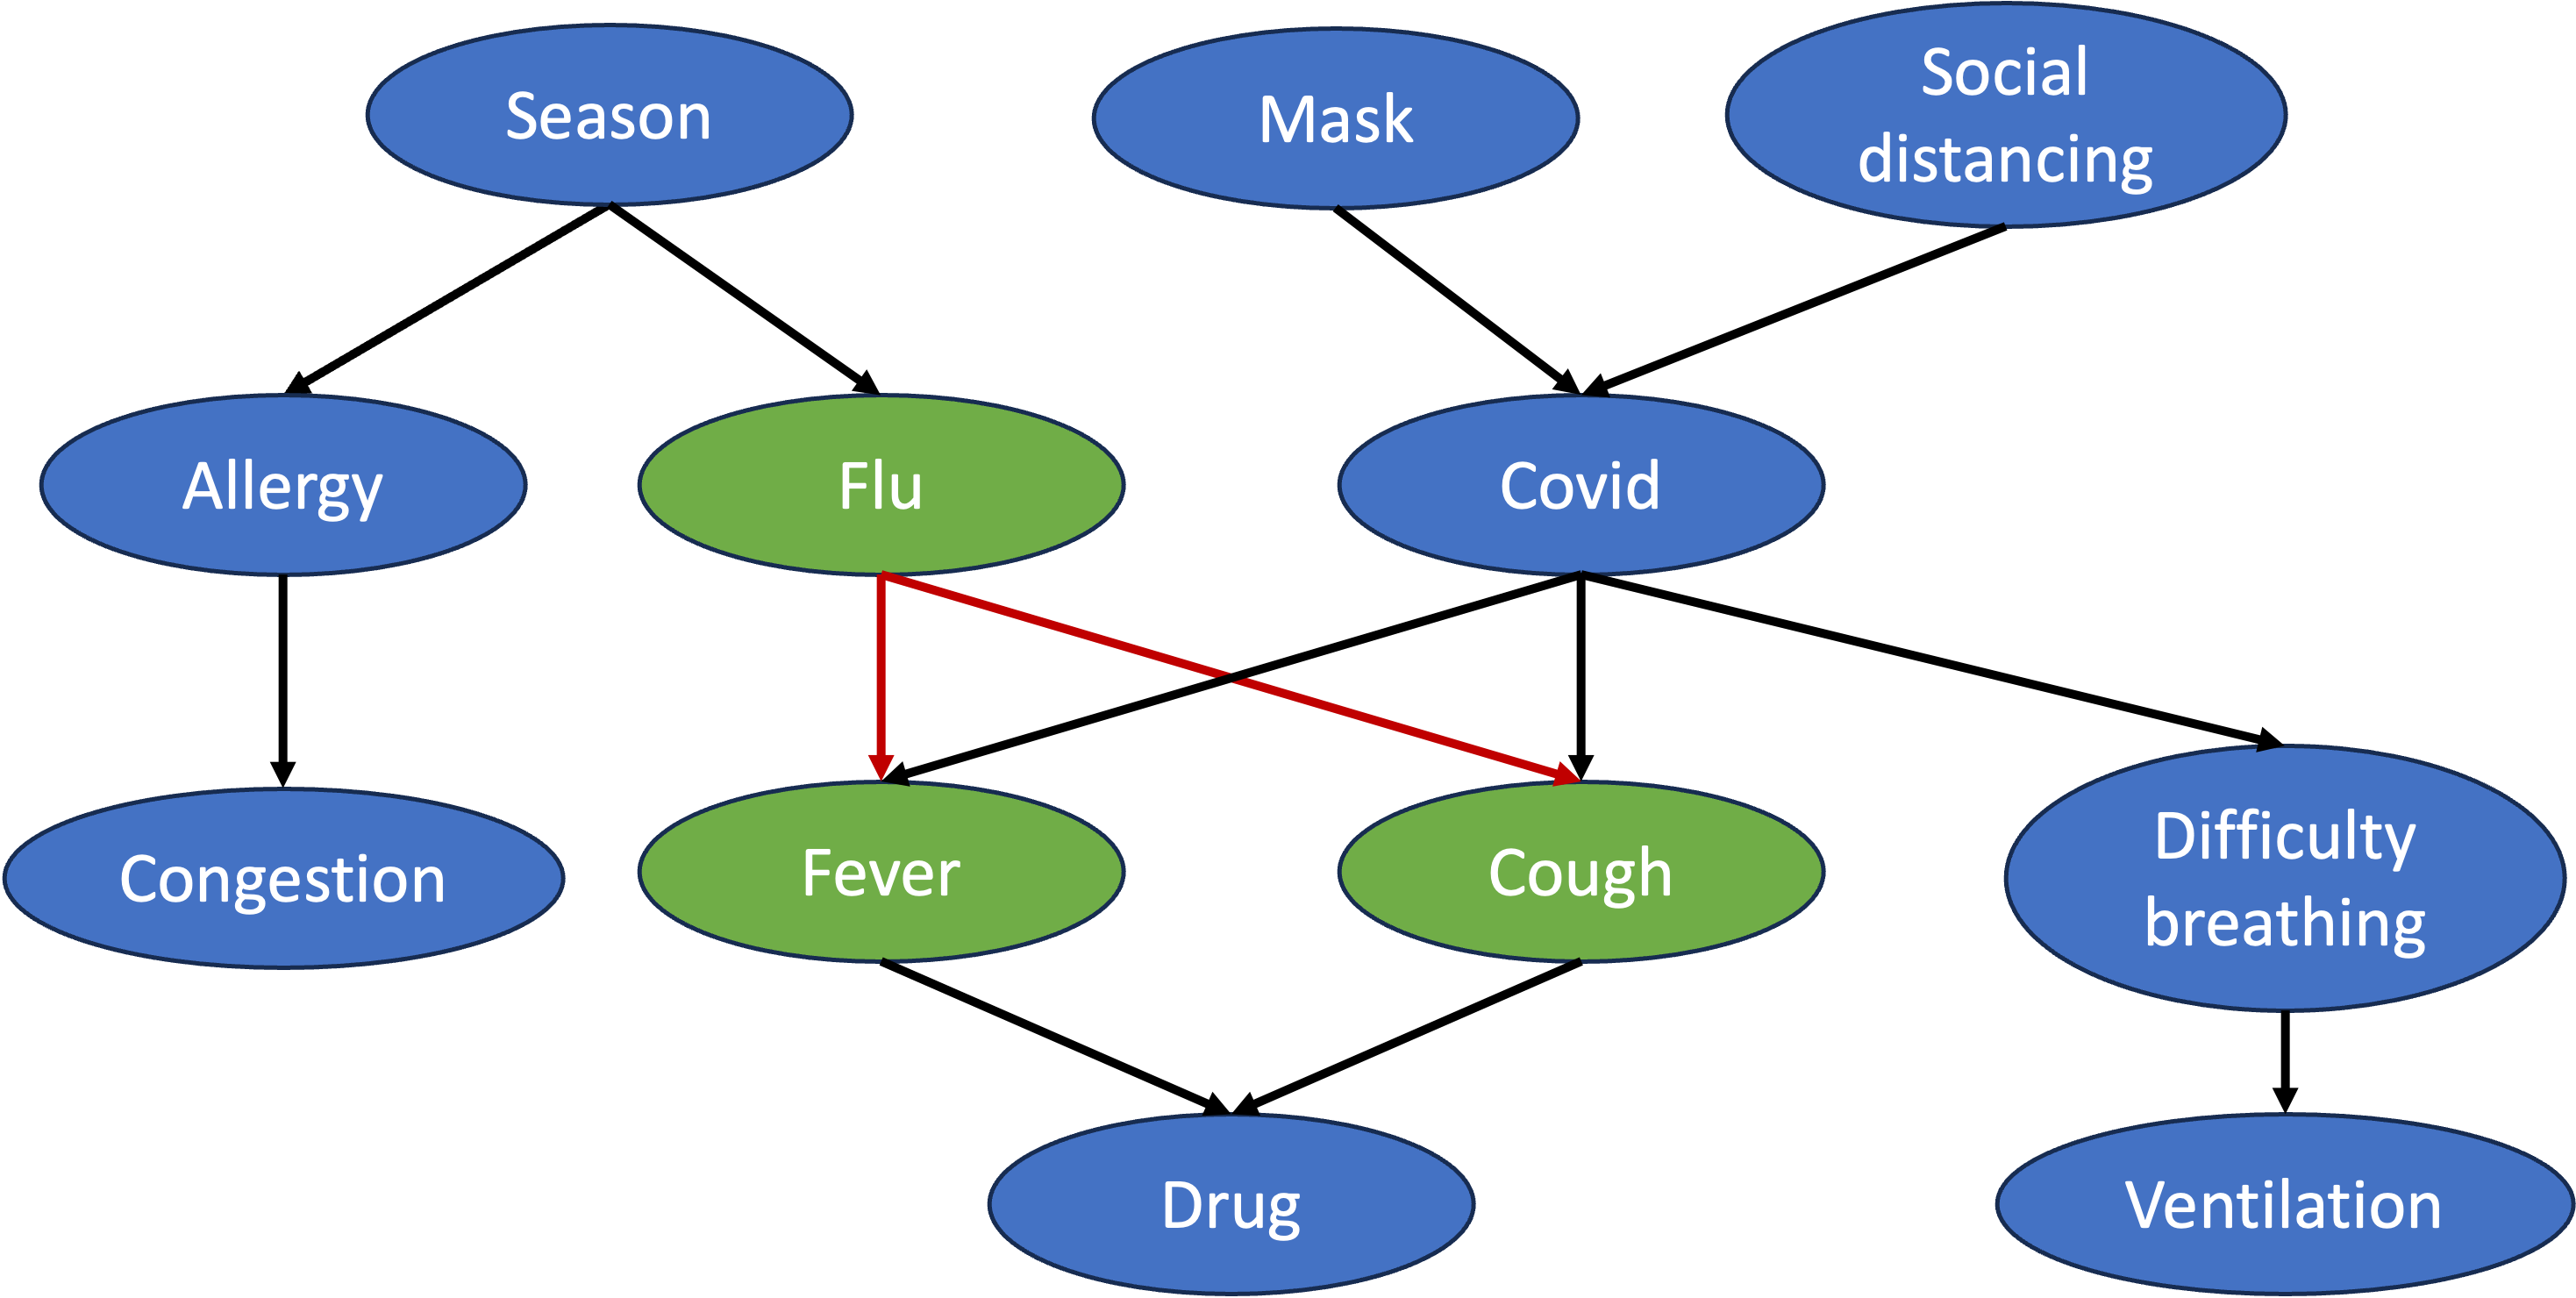
\includegraphics[width = 13cm, height = 6cm]{active_covid.png}
        \end{center}
        \vspace{1cm}
        \item If Z = {Flu} => inactive trail 
        \begin{center}
            Once we know the person has flu, fever gives no additional information about cough.
            \vspace{0.5cm}
            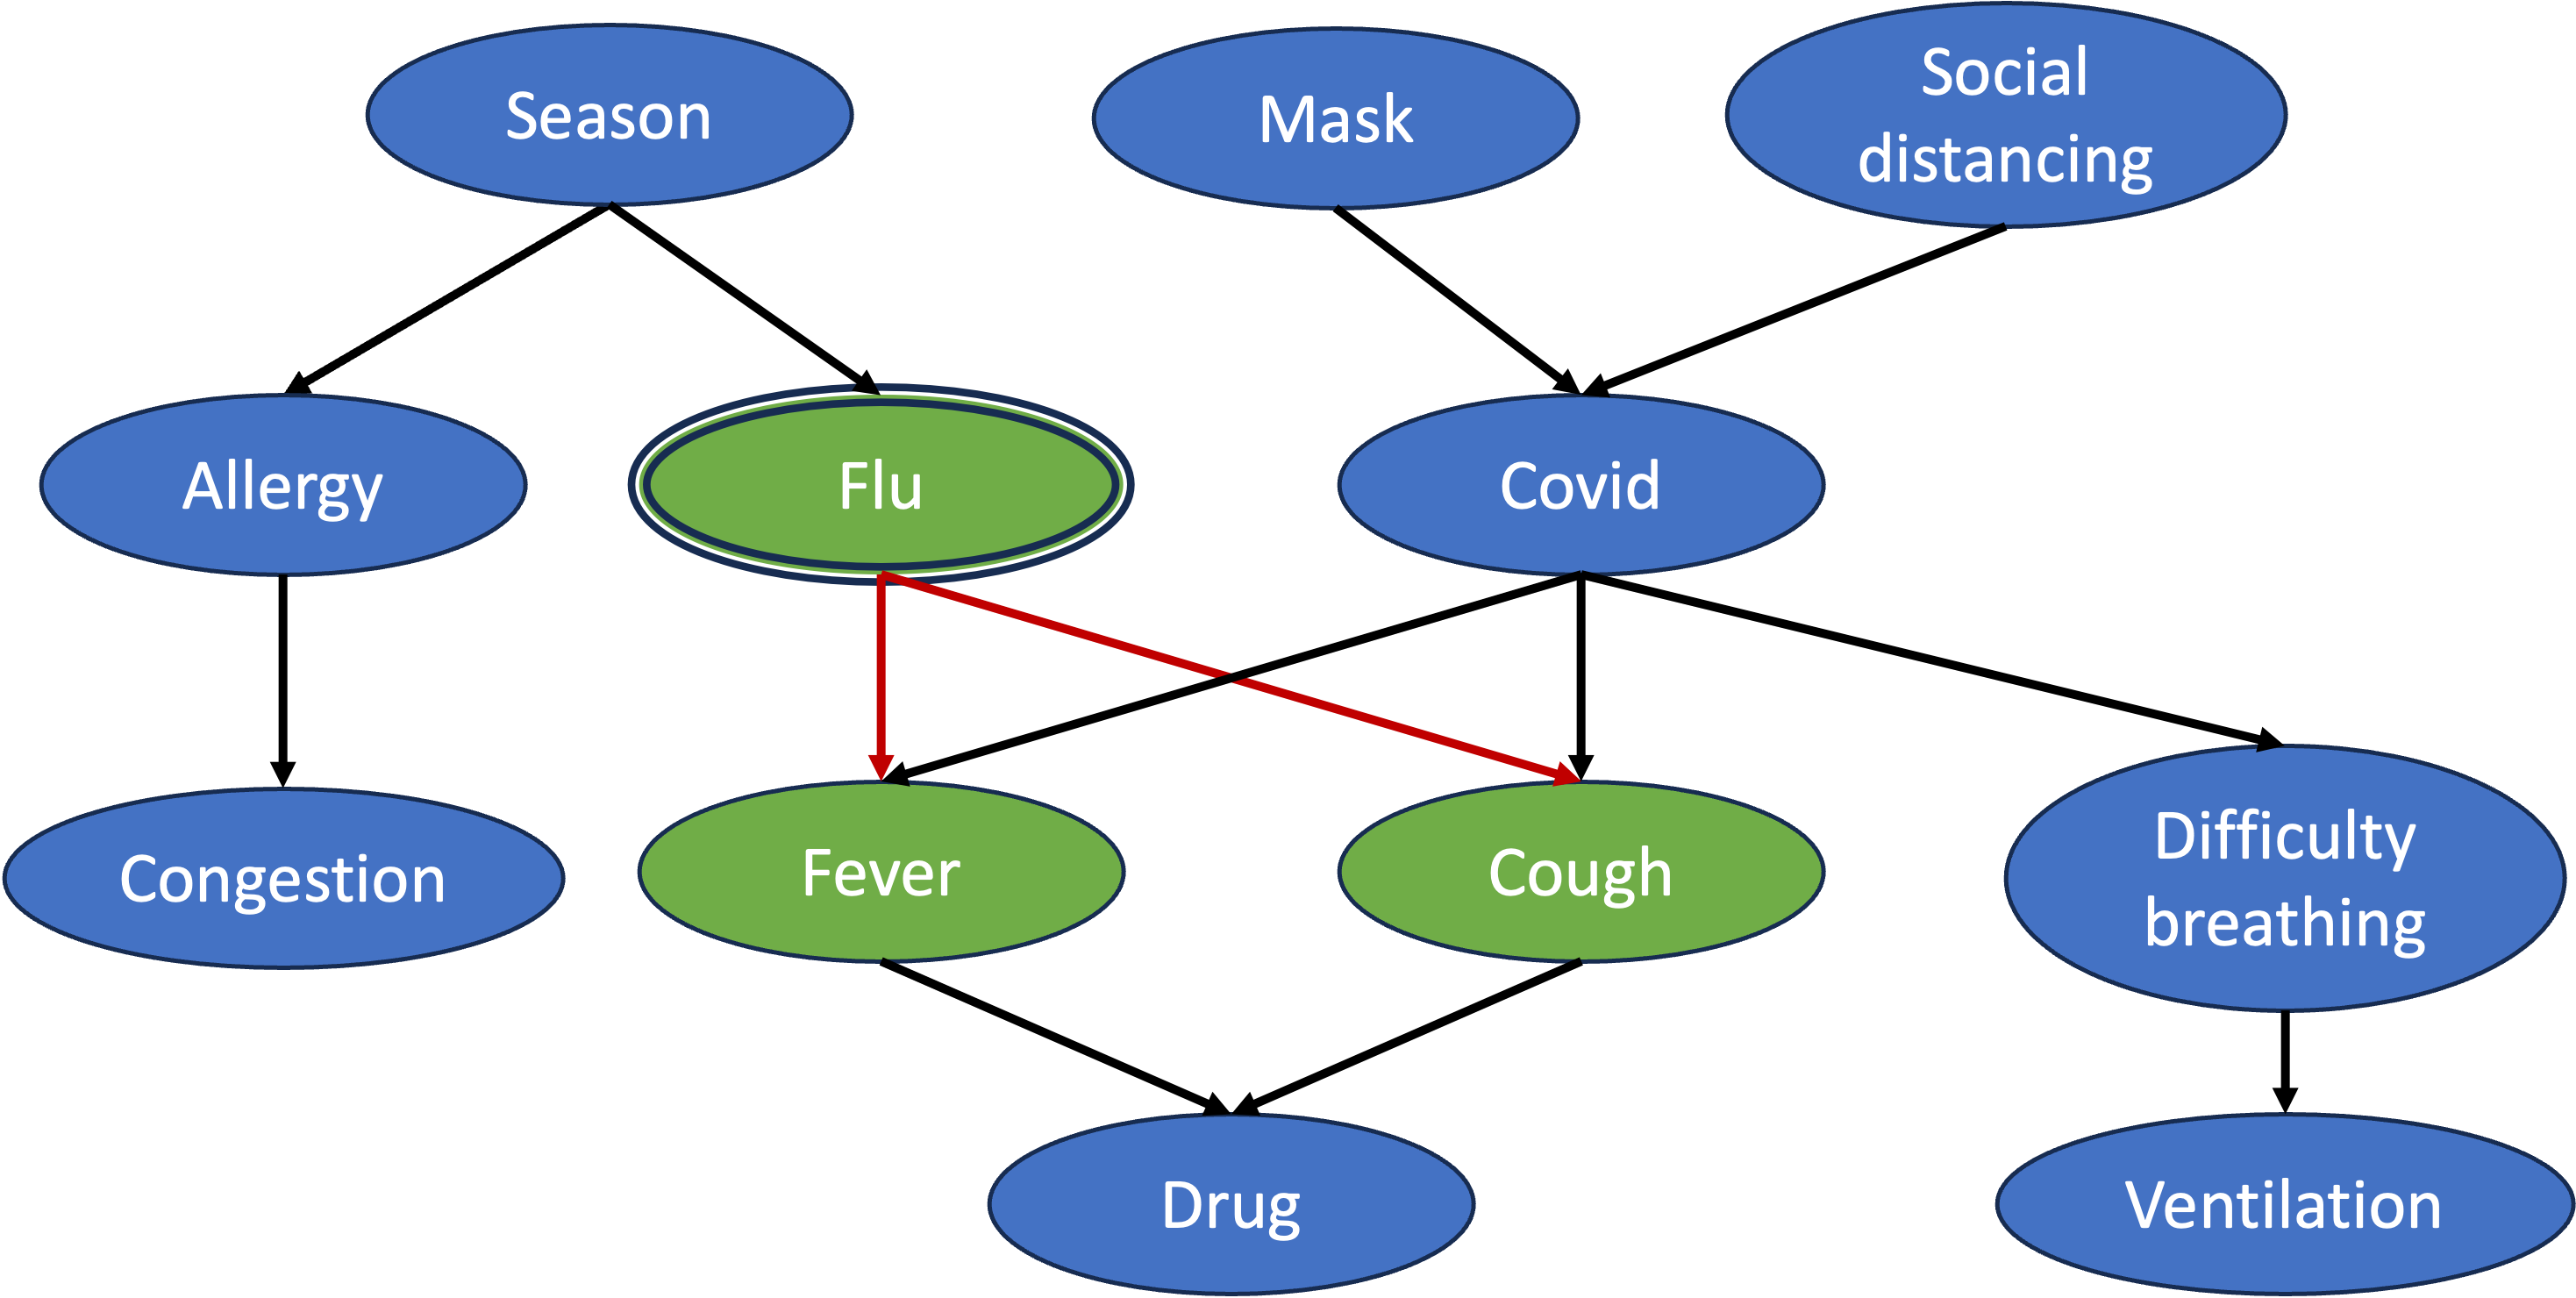
\includegraphics[width = 13cm, height = 6cm]{inactive_covid.png}
            \end{center}
    \end{itemize}
    \item V-structure Example: Consider the trail Flu -> Fever <- Cough in the covid example
    \begin{itemize}
        \item If $Z = \emptyset$ => inactive trail
        \begin{center}
        having flu, does not make a person more or less likely to have covid. So, no information flows along the trail.
        \vspace{0.5cm}
        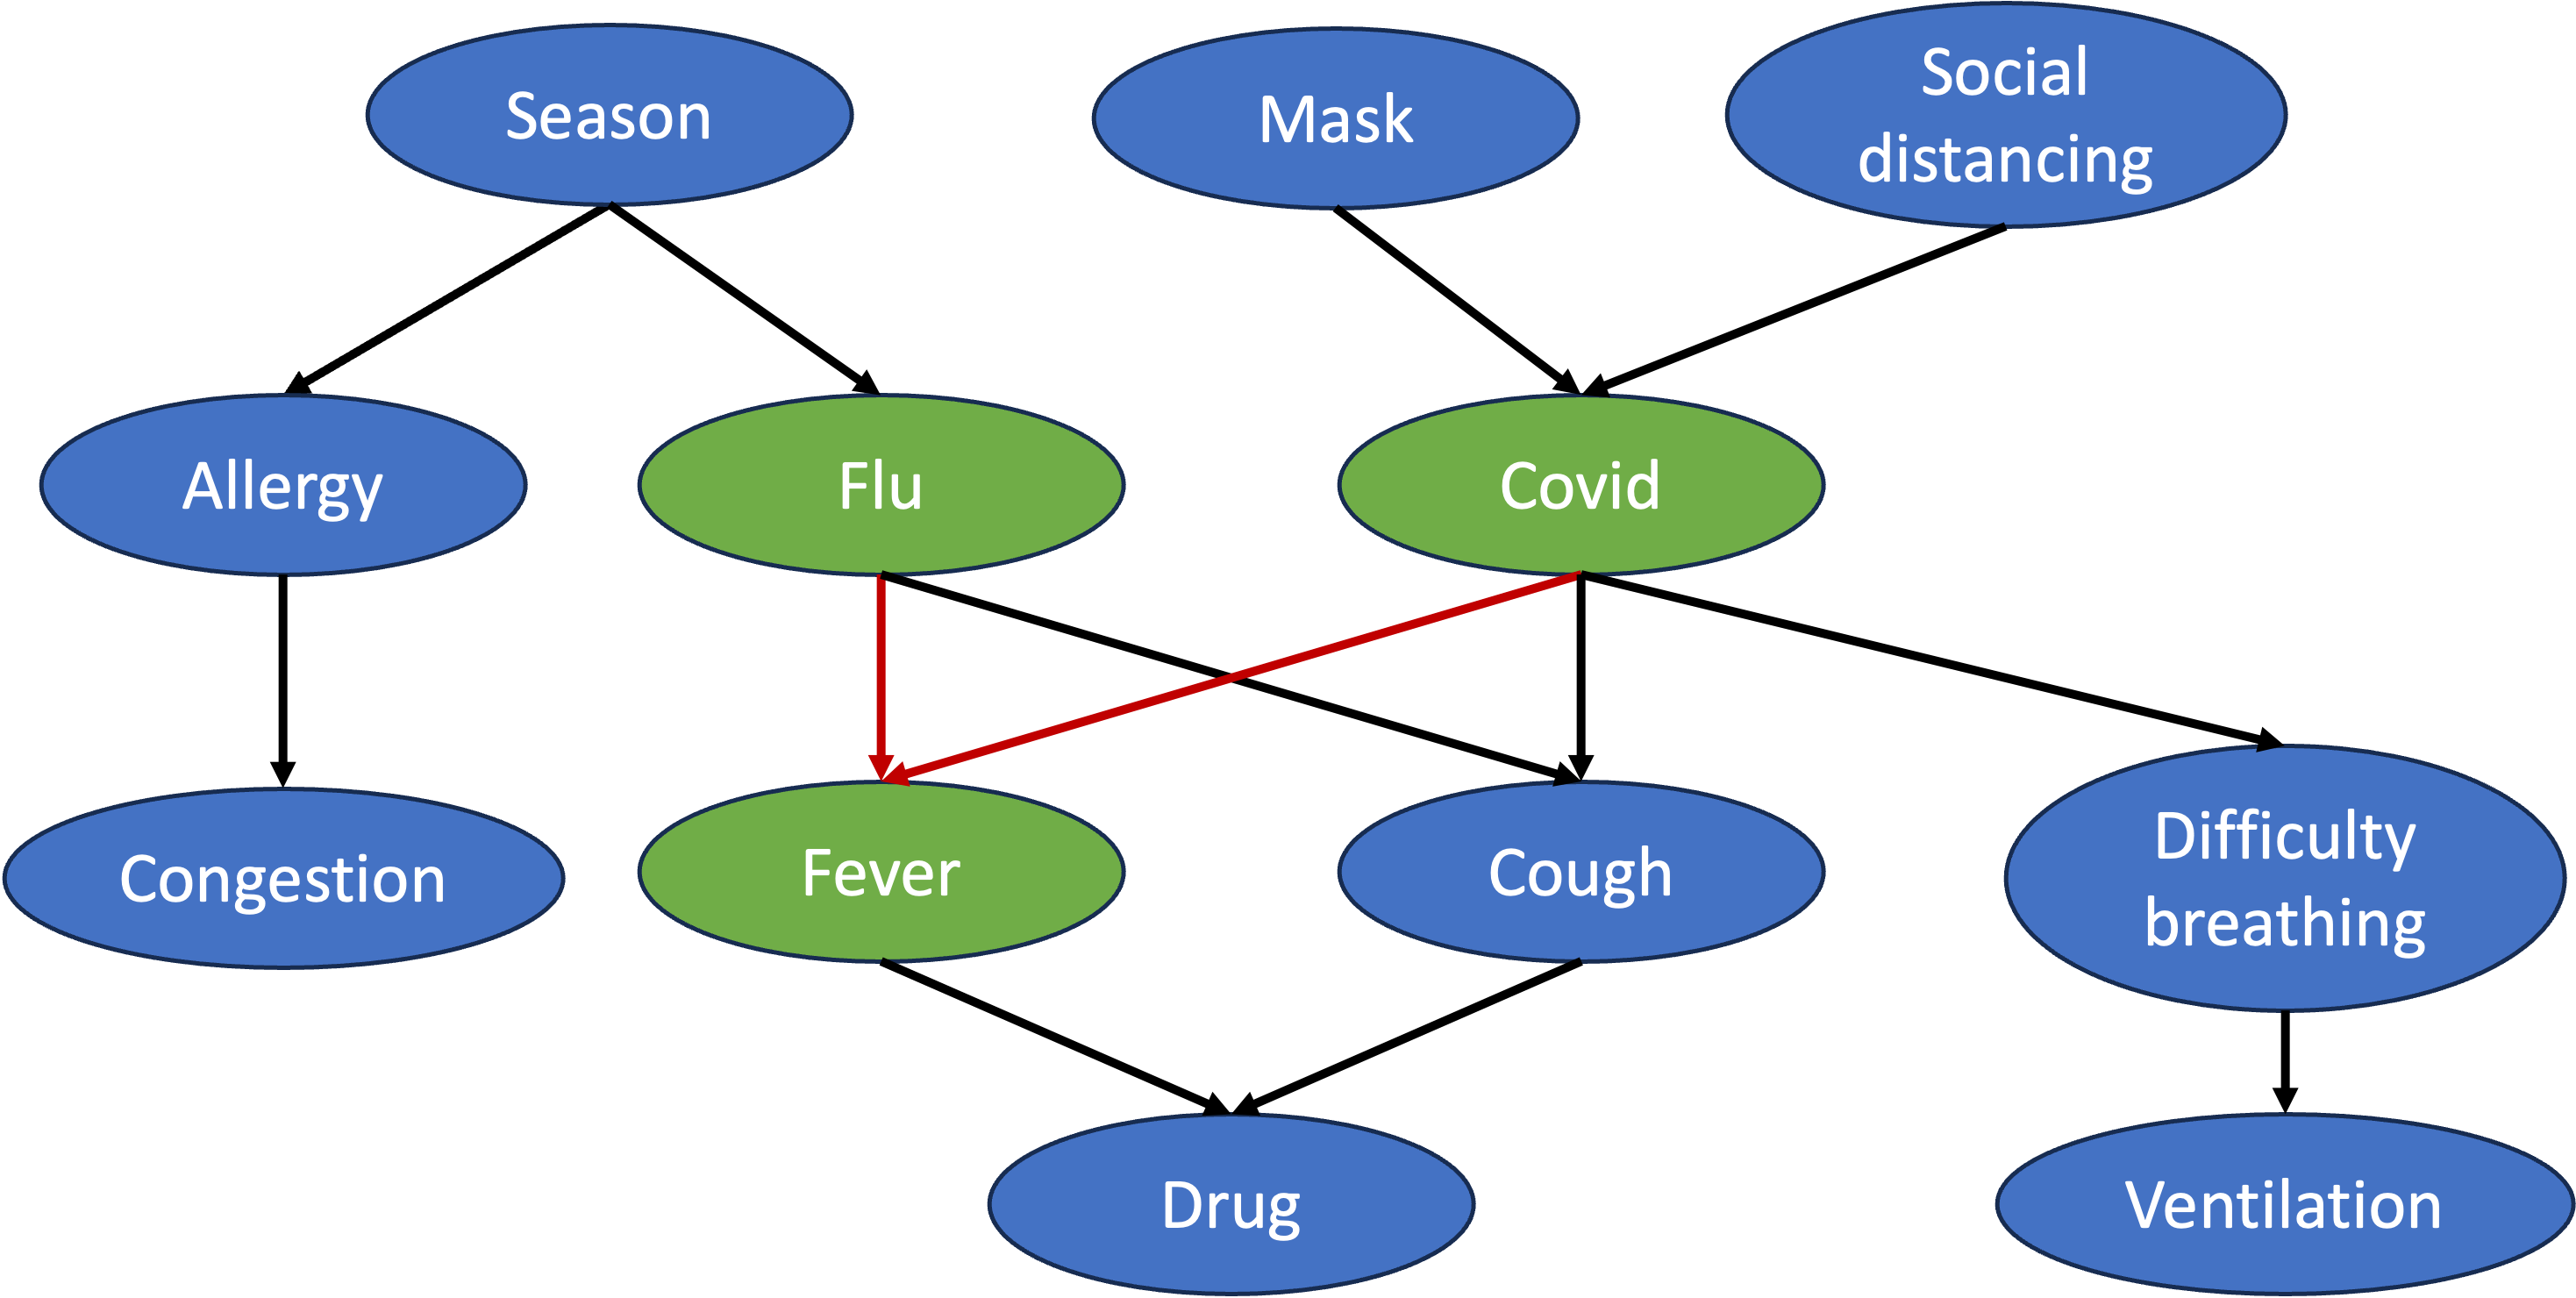
\includegraphics[width = 13cm, height = 6cm]{inactive_covid_v.png}
        \end{center}
        \vspace{1cm}
        \item If Z = {Fever} => active trail 
        \begin{center}
            Flu and covid become dependent. If a person is known to have fever, then she/he is likely infected with covid if not having flu and vice versa.
            \vspace{0.5cm}
            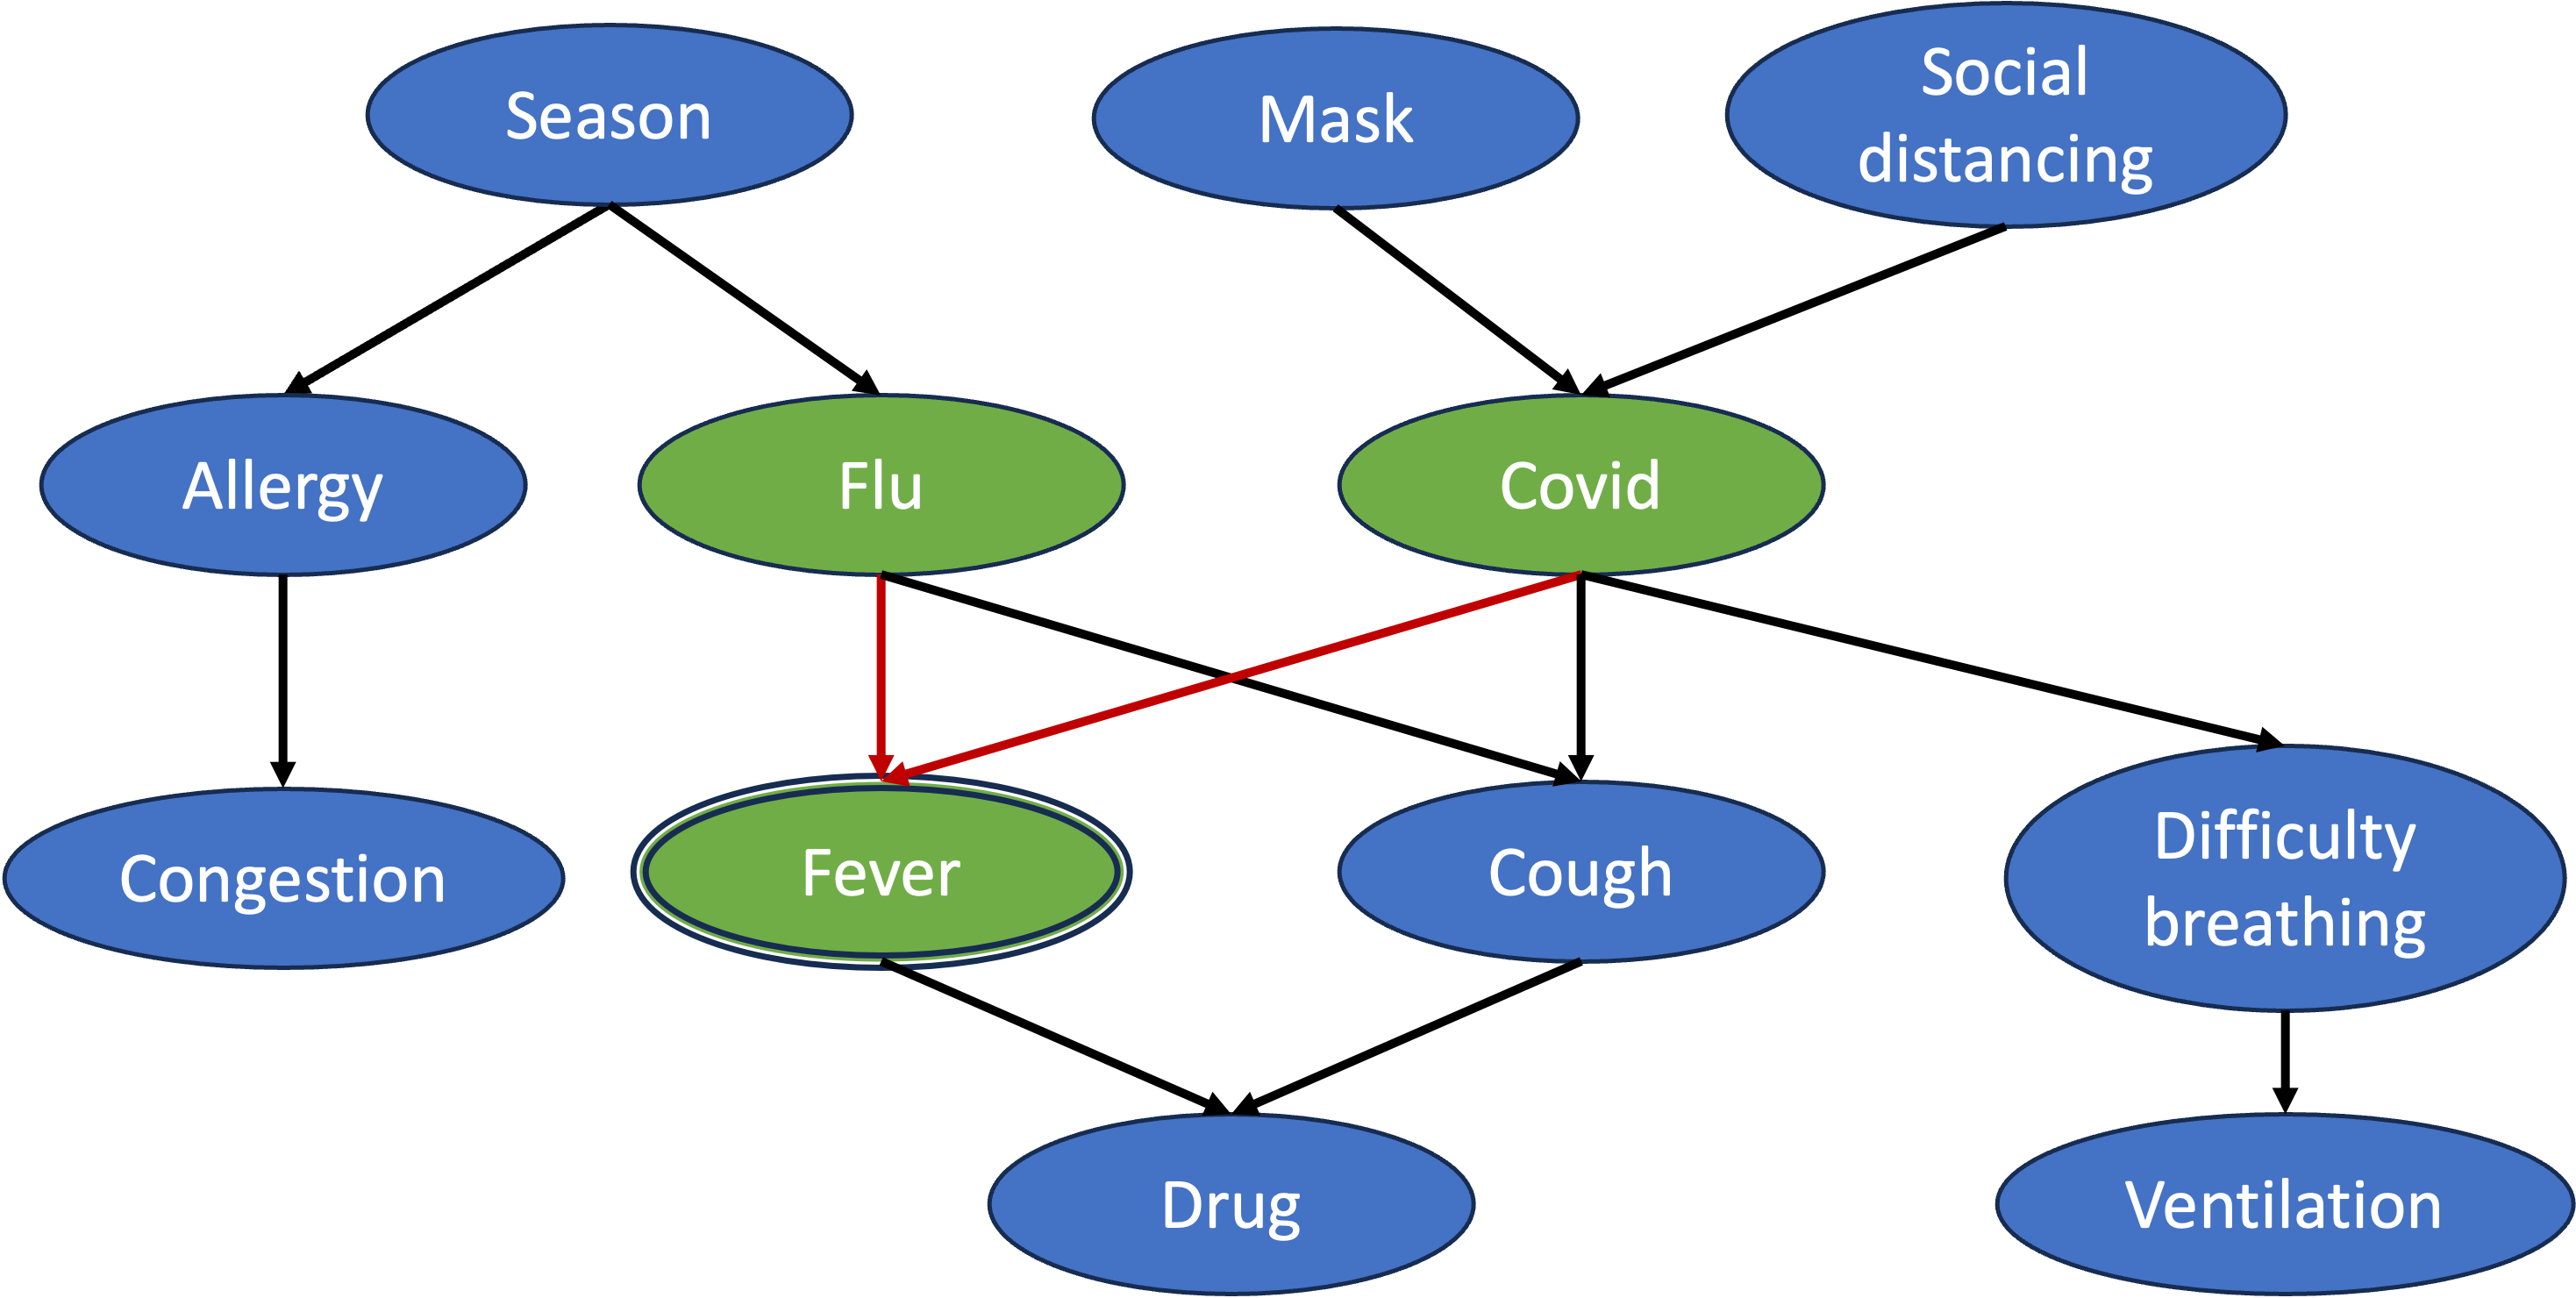
\includegraphics[width = 13cm, height = 6cm]{active_covid_v.png}
            \end{center}
    \end{itemize}
    \item Active trails
    \begin{center}
    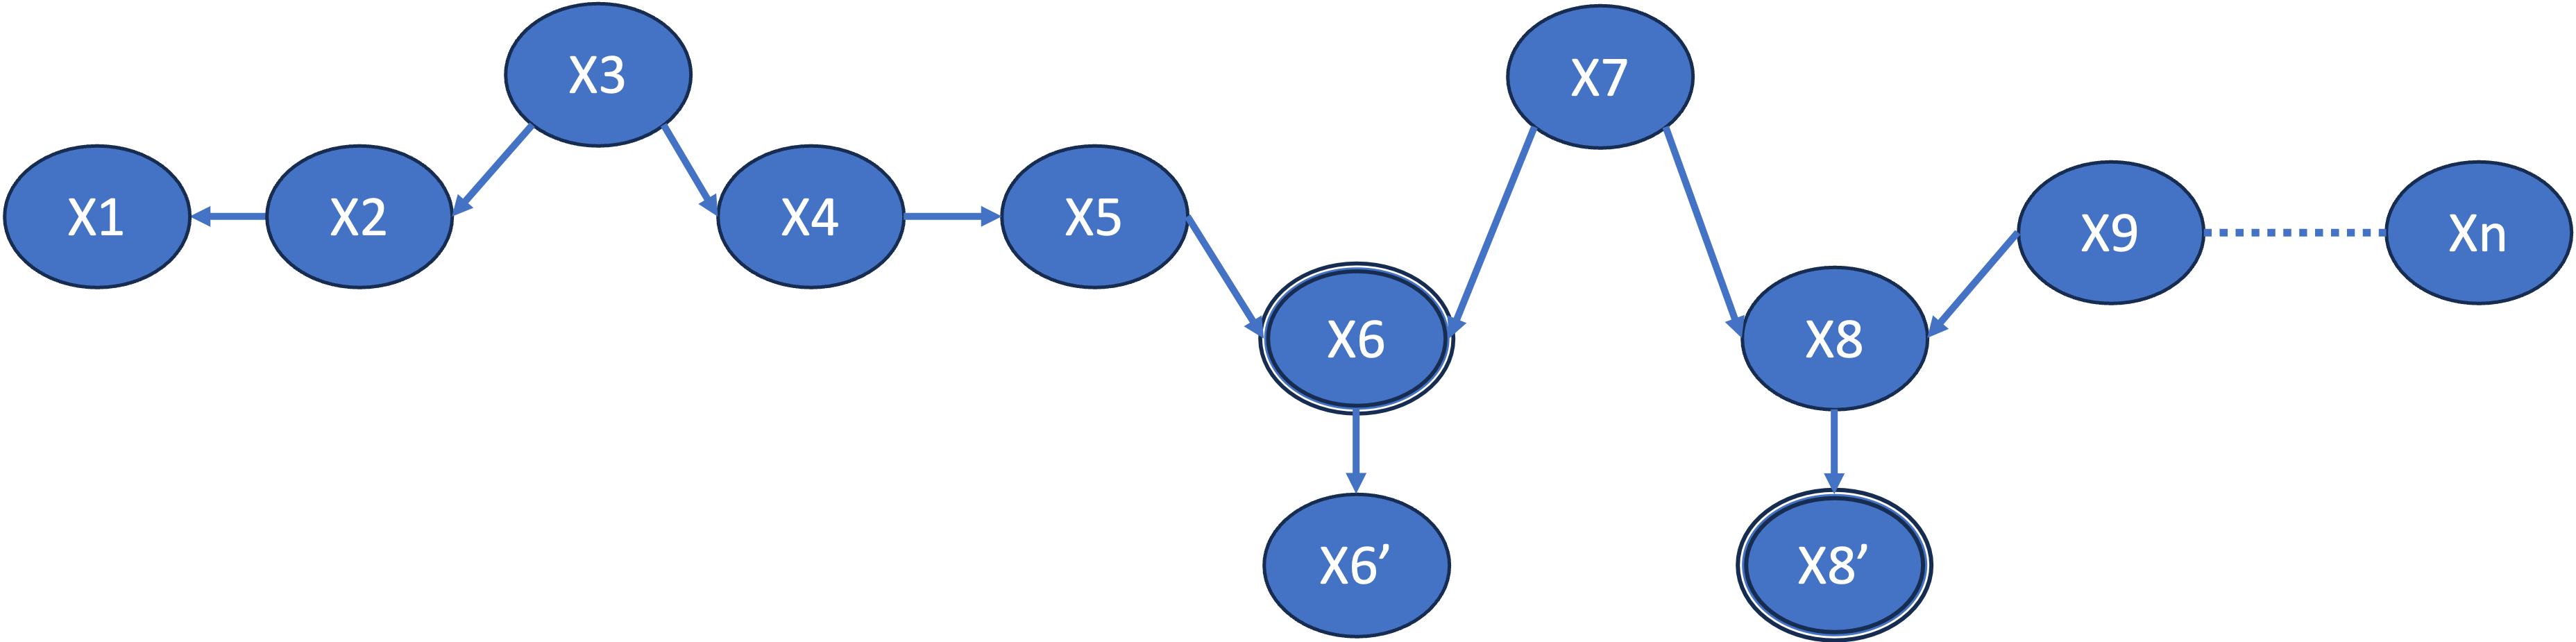
\includegraphics[width = 15cm, height = 3cm]{active_trail.png}
    Put all the nodes on a horizontal line. Move common cause above the line and v-structure below the line. In an active trail, \textbf{exactly the nodes at the bottom lines are observed}. Only sinks could and should be observed.
    \end{center}
    \item Definition
    \begin{itemize}
        \item Active trail
        \begin{center}
             Let Z be the set of observed variables. Trail x1 <=> \ldots <=> xn in G is active given Z if: 1. For any v-structure Xi-1 -> Xi <- Xi+1, either Xi or one of its descendants are in Z. 2. No other node along the trail is in Z.
        \end{center}
        \item In order to have global conditional independence, all trails must be inactive (no information flow).
        \item Inactivity implies independence: Given observed Z, if there is no active trail between the nodes X and Y in graph G, then X and Y are independent given Z under any probability distribution that factorize according to G.
    \end{itemize}
\end{itemize}

\section{d-separation}

\begin{itemize}
    \item D(dependence)-separation definition
    
    In a graph G, two sets of nodes X and Y are d-separated given the set Z, denoted \begin{center}
        $d-sep{G}(X; Y \mid Z)$
    \end{center}, if there is no active trail between any node $x \in X$ and any node $y \in Y$ given Z.

    \item Covid example

    Consider the sets X = {Season, Allergy, Flu, Congestion} and Y = {Mask, Social distancing, COVID, Diffulty breathing, Ventilation}.
    \begin{itemize}
        \item If $Z = \emptyset$, all trails are inactive

        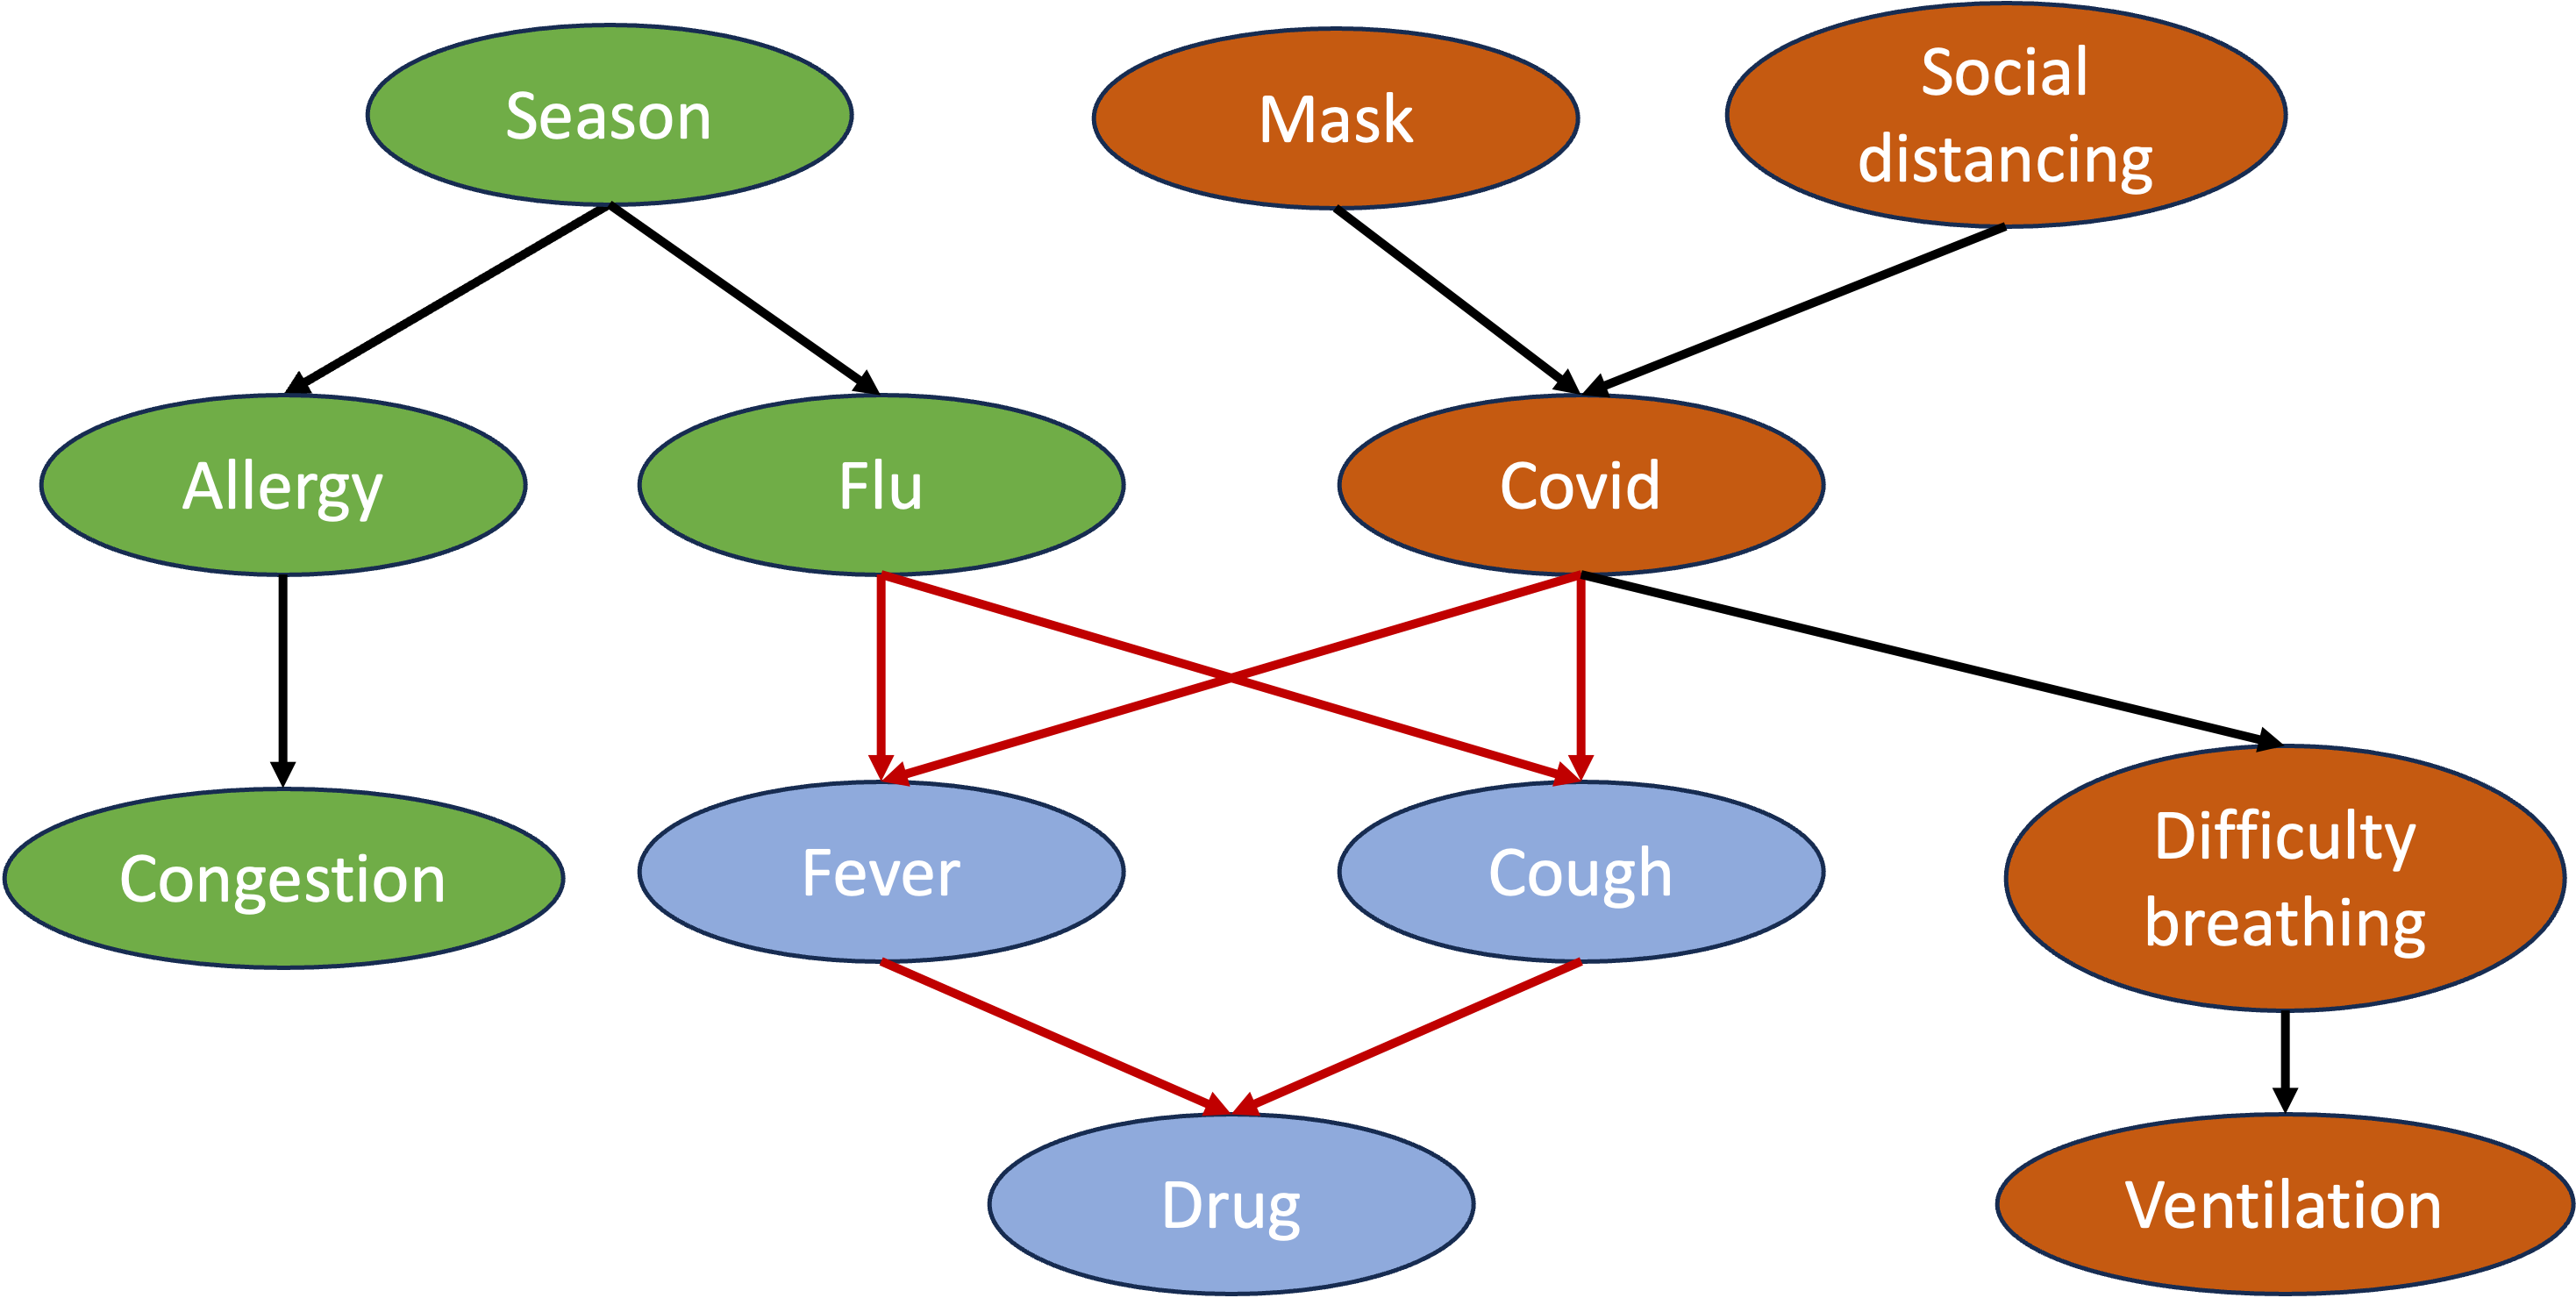
\includegraphics[width = 12cm, height = 6cm]{d_seq_inactive.png}
        \item If $Z = \{fever\}$, there exists an active trail.
       
        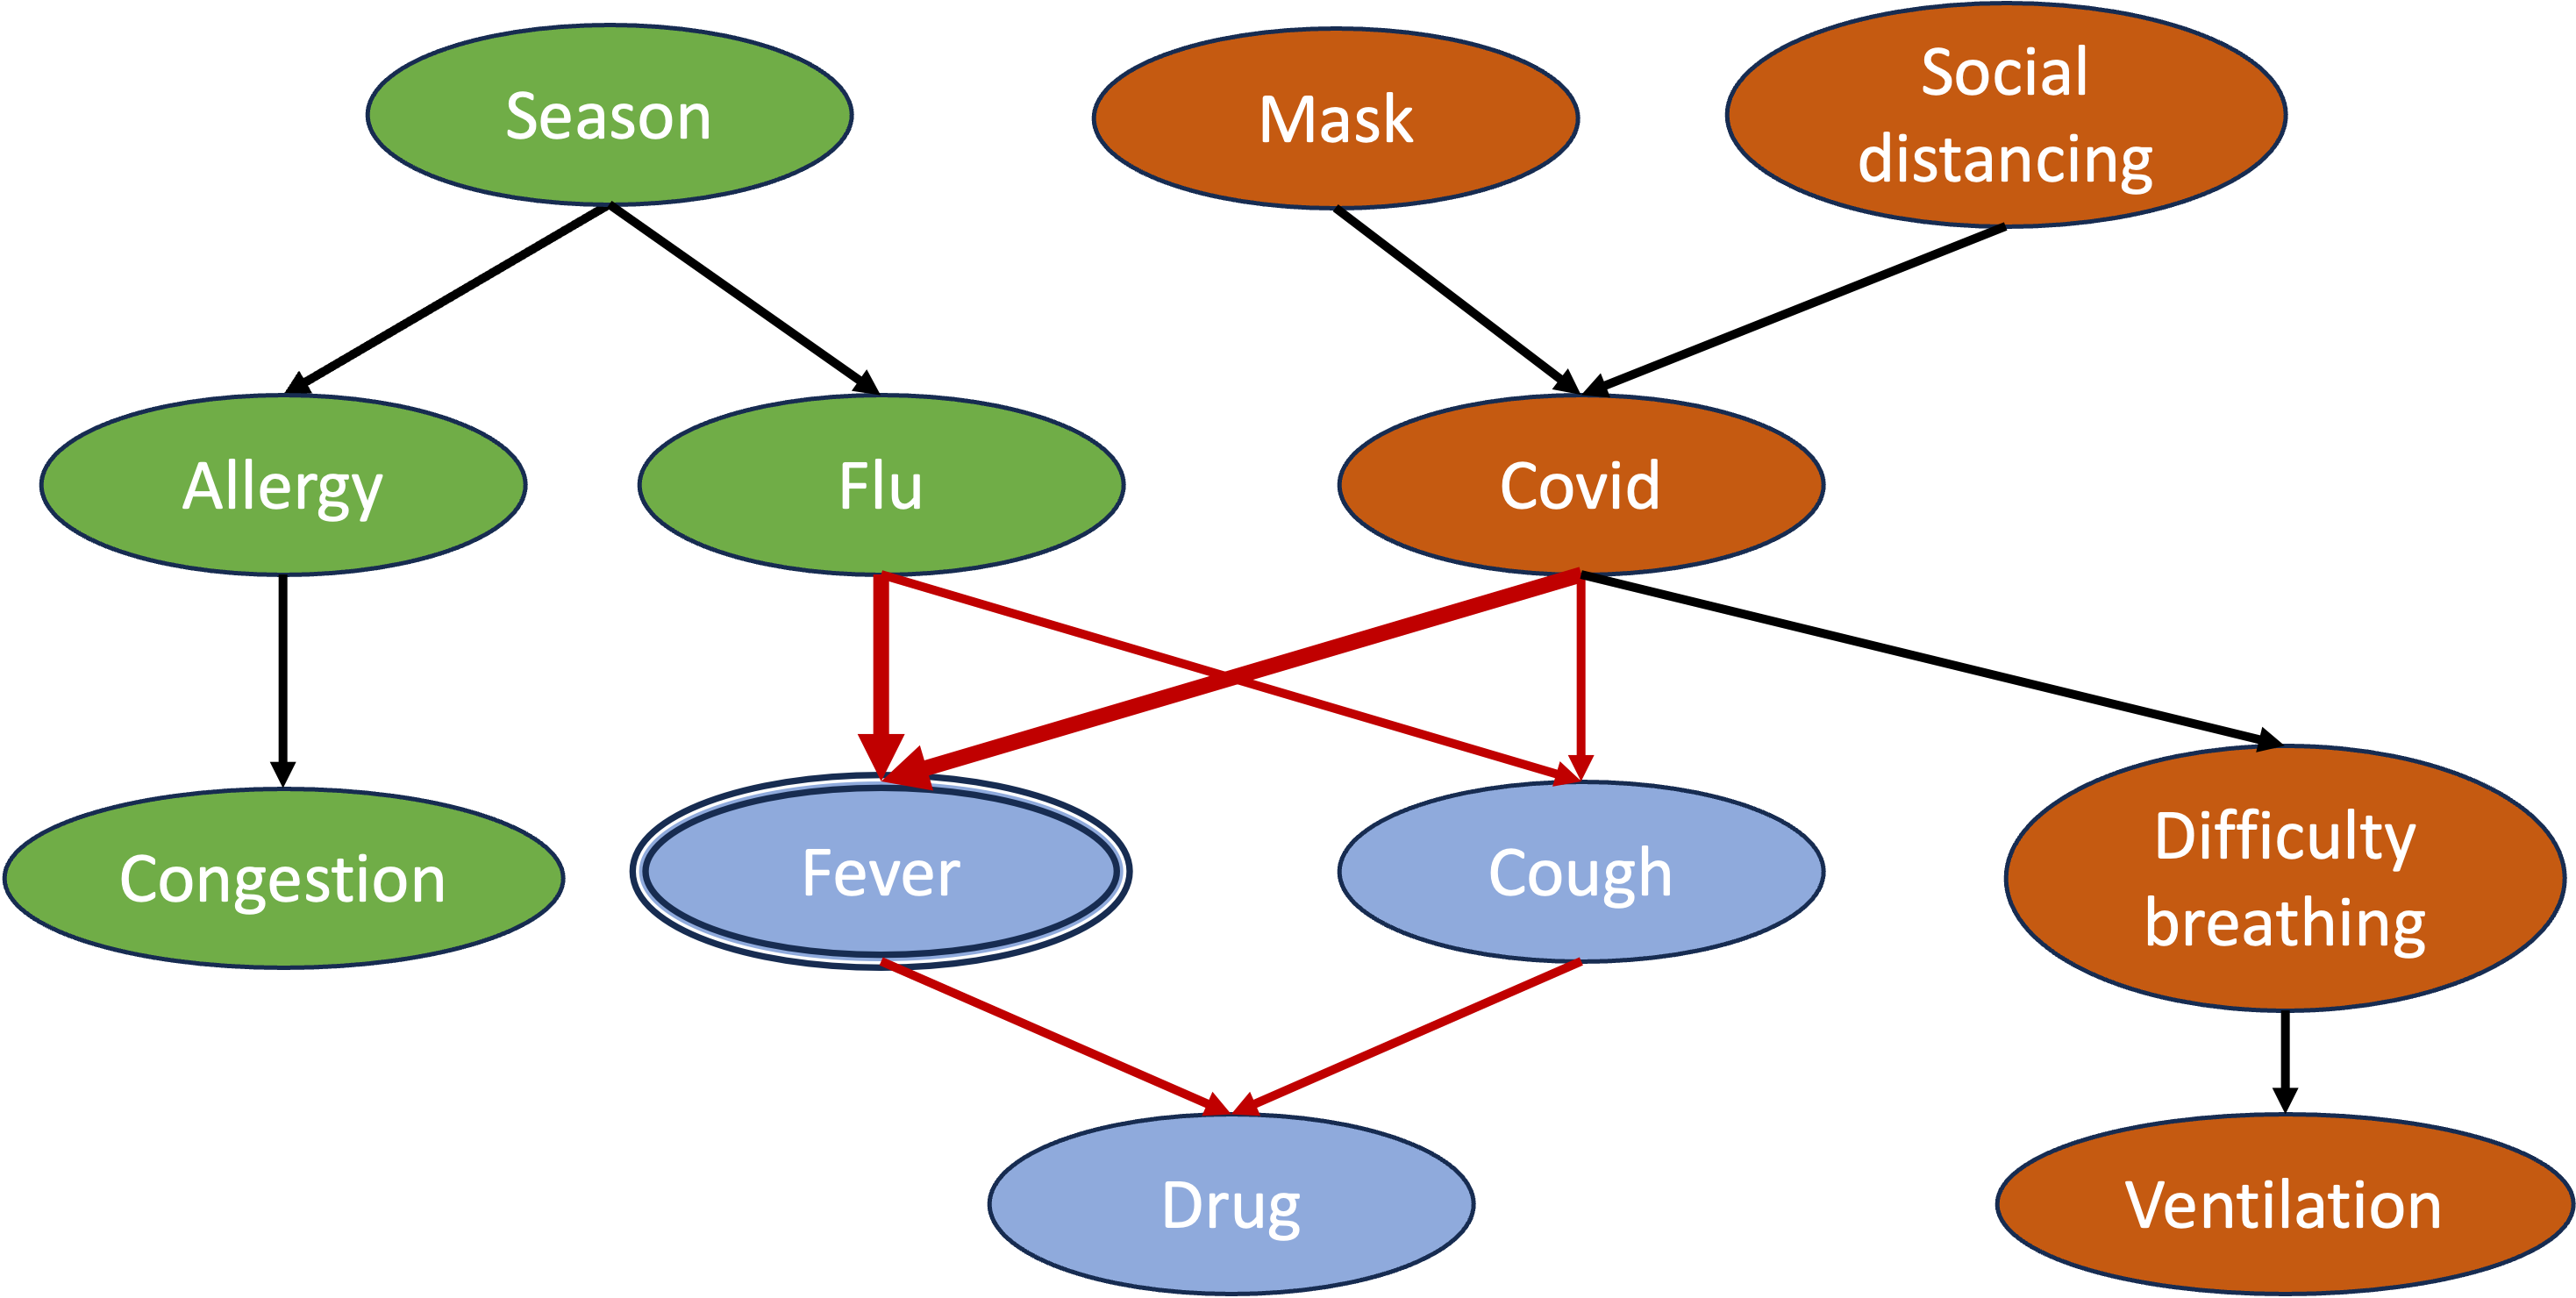
\includegraphics[width = 12cm, height = 6cm]{d_seq_active.png}
    \end{itemize}

    \item Definition: Global Markov Independence 
    
    The set of independencies resulting from d-separation is defined as the set of global markov independencies.

    \begin{center}
        $I(G) = {(X \perp Y \mid Z): d-sep_{G}(X; Y \perp Z)}$
    \end{center}

    \item Theorem

    \begin{center}
        If a distribution P factorizes according to G, then $I(G) \subseteq I(P)$.\\

        $I_{l}(G) \subseteq I(P) => I(G) \subseteq I(P)$\\
        i.e., if the local independencies are satisfied by P, so are the global.
    \end{center}

    \item Example
    
    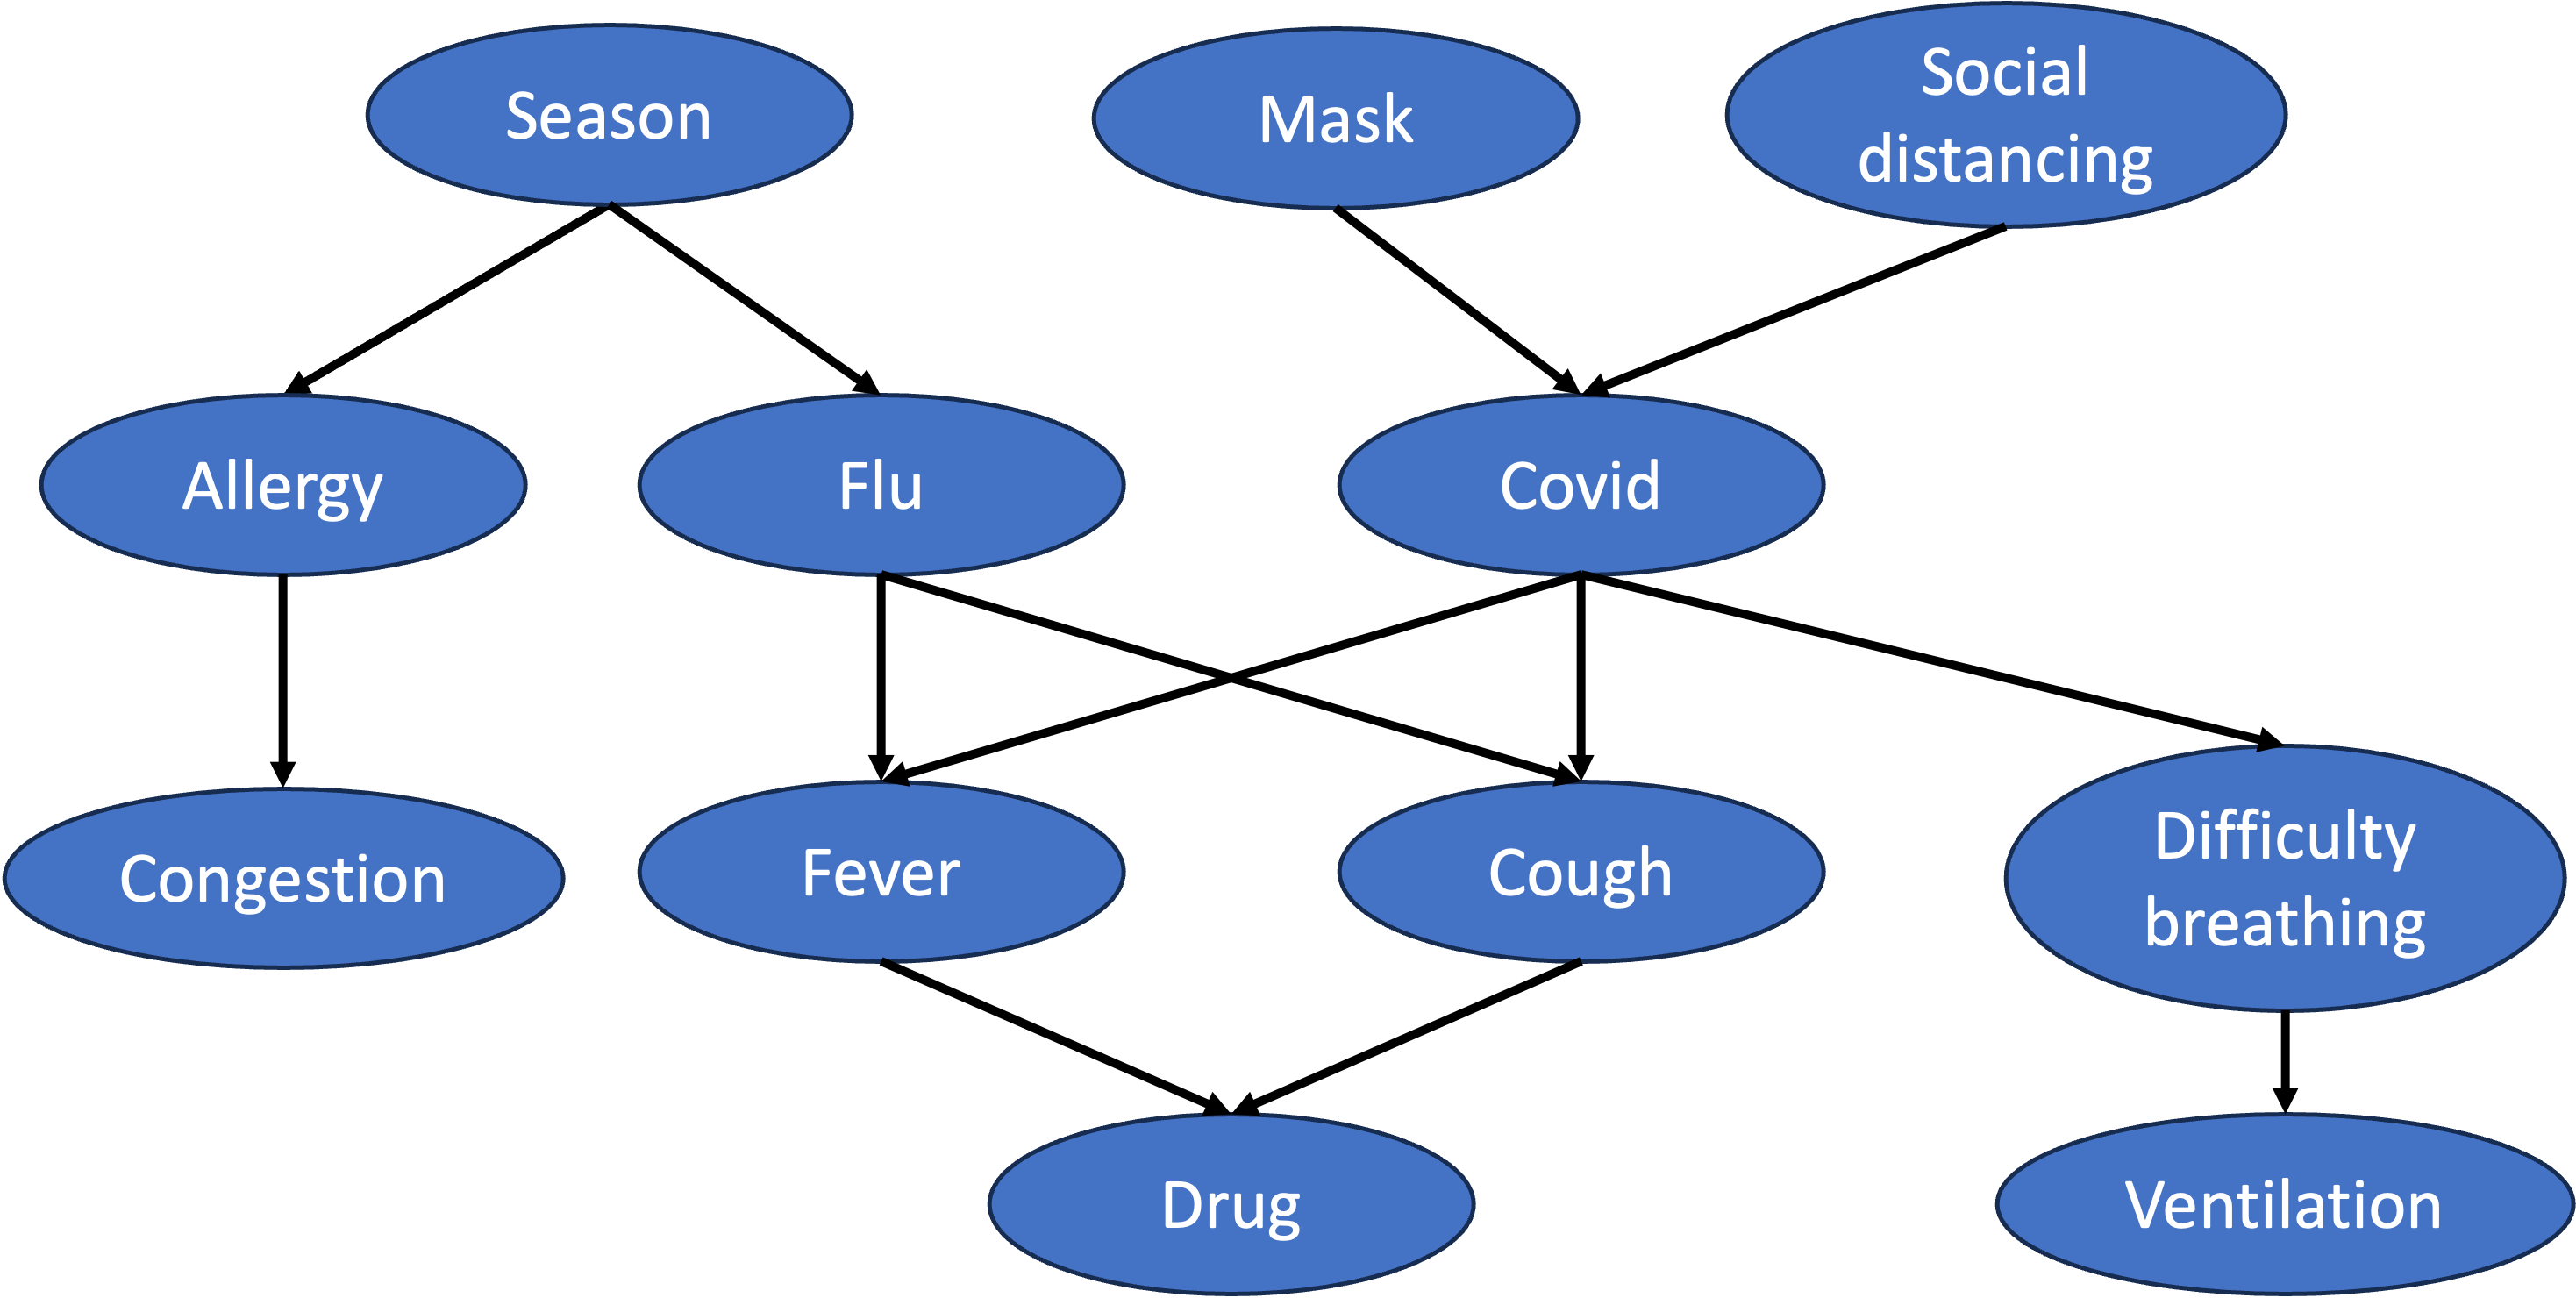
\includegraphics[width = 12cm, height = 6cm]{bn_global_indep.png}
    \begin{itemize}
        \item Assume that the true joint probability distribution P of random variables satisfies the previously stated indepencies.
        \item Is the graph an i-map for P? Does P factorize according to the graph? yes
        \item Does the factorization impose any independence in addition to the previously stated one? yes, but P satisfied them all.
    \end{itemize}
\end{itemize}

\section{Summary: What is the Goal?}

The goal is to find from data, the correct factorization of the joint probability distribution. 

\begin{itemize}
    \item First, finding the conditional independence I(P)
    \item For each factorization, we could draw a bayesian nets, and we could write down local independencies $I_{l}^{G}$. If $I_{l}^{G} \subseteq I(P)$, then G is I\_map for P
    \item There could be several i\_map for P, which one to choose? The minimal I-maps
    \item Does P satisfy all global independencies imposed by the minimal I-maps? yes
\end{itemize}

%%------------------------------- chapter ------------------------------------

\chapter{P-map}

\section{$I(G) \stackrel{?}{=} I(P)$}

\begin{itemize}
    \item Recall from last chapter: If a distribution P factorizes according to G, then $I(G) \subseteq I(P)$. It means that all independencies implied by G are also included in P.
    \item The question now is can P have an independence not included in G? The answer is Yes.
    \item Can we conclude I(P) = I(G)? No, but almost yes.
    \item Theorem of Completeness
    \begin{center}
        For almost all distributions P that factorize over G, except for a set of measure zero in the space of CPD parameterizations, I(G) = I(P)
    \end{center}
\end{itemize}

\section{P-map}

\begin{itemize}
    \item Definition: Graph G is a perfect map (P-map) for P if I(P) = I(G).
    \item Consider the joint distribution P over $X_{1}, X_{2}, \ldots, X_{4}$, where
    \begin{center}
        I(P) =  {$(X_{4} \perp X_{2}, X_{1} \mid X_{3})$ and its derivations}
    \end{center}
    \begin{itemize}
        \item Graph1
        
        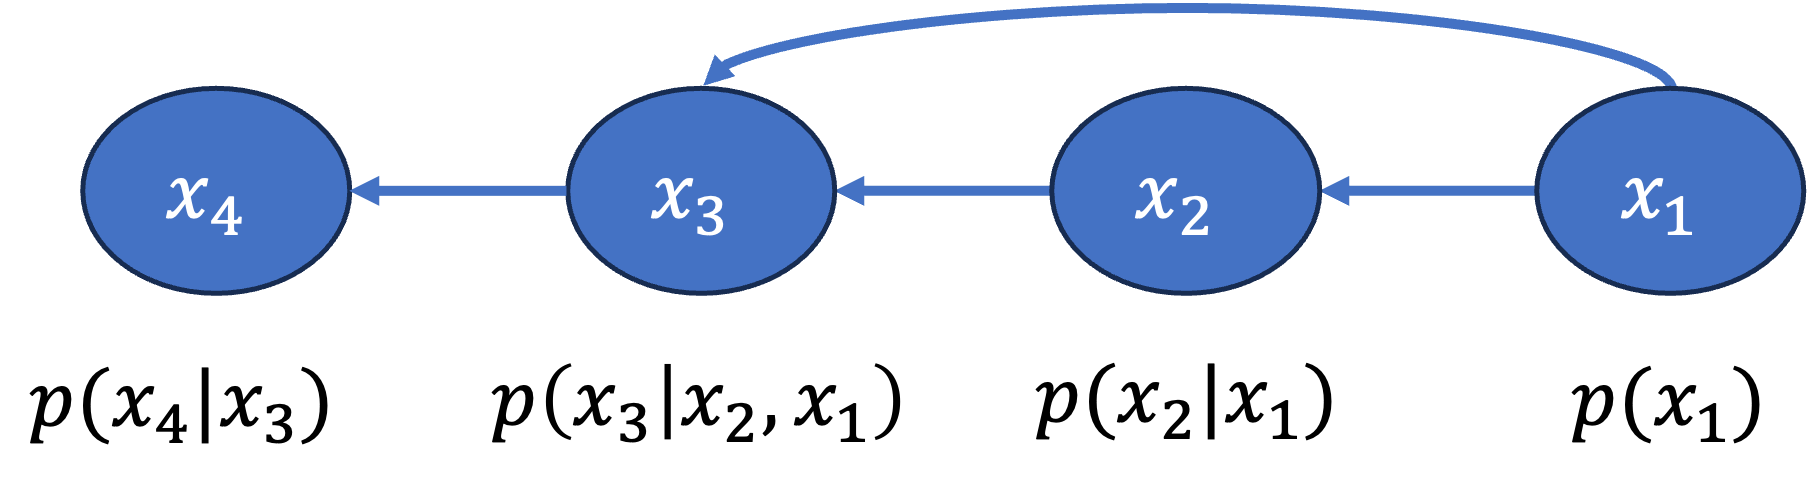
\includegraphics[width = 10cm, height = 3cm]{graph_vis.png}\\
        $I_{l}(G_{1}) = {(X_{4} \perp X_{2}, X_{1} \perp X_{3})}$\\
        Therefore, $I(G_{1}) = I(P)$, $G_{1}$ is an p-map for P.

        \item Graph2
        
        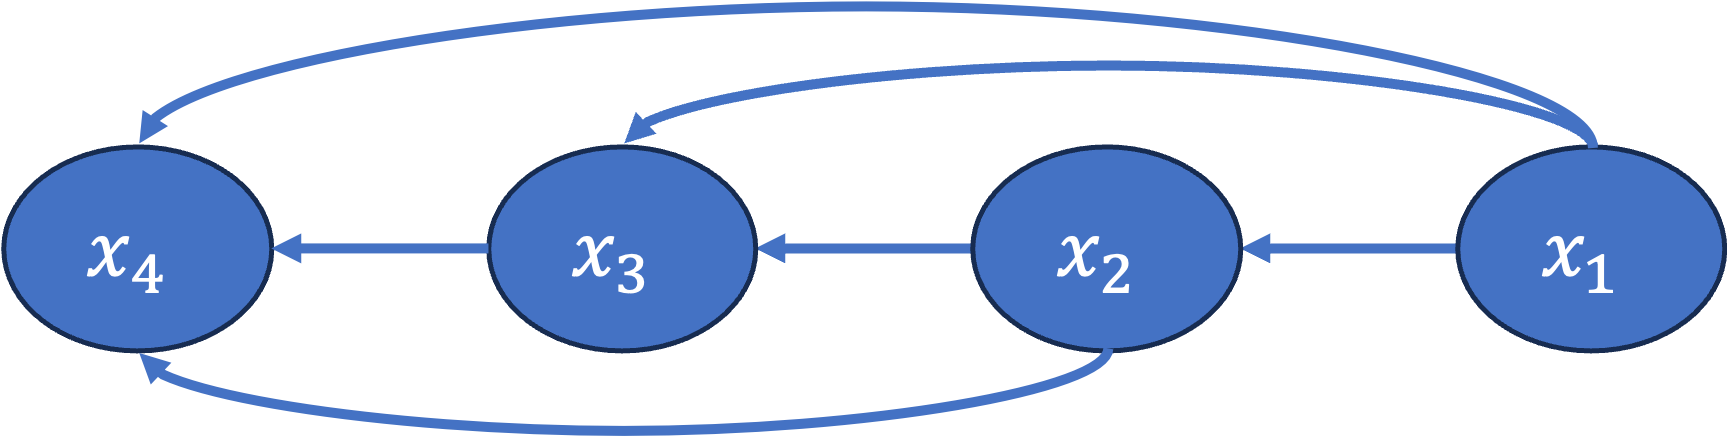
\includegraphics[width = 10cm, height = 3cm]{graph_vis2.png}\\
        $I_{l}(G_{2}) = \emptyset $\\
        Therefore, $I(G_{2}) \subseteq I(P)$, $G_{2}$ is not a p-map for P.

        \item Graph3
        
        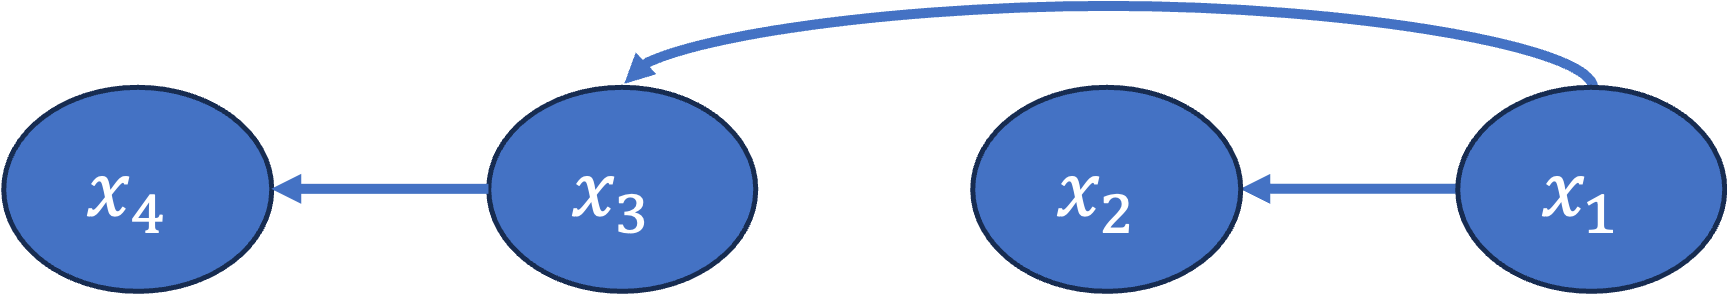
\includegraphics[width = 10cm, height = 2cm]{imap_1.png}\\
        $(X_{3} \perp X_{2} \mid X_{1}) \in I_{l}(G_{3})$
        $(X_{3} \perp X_{2} \mid X_{1}) \notin I(P)$
        Therefore, $G_{3}$ is not an i-map for p and not a p-map for p.
    \end{itemize}
\end{itemize}

\section{Summary: What is the Goal?}

The goal is to find from data, the correct factorization of the joint probability distribution. 

\begin{itemize}
    \item First, finding the conditional independence I(P)
    \item For each factorization, we could draw a bayesian nets, and we could write down local independencies $I_{l}^{G}$. If $I_{l}^{G} \subseteq I(P)$, then G is I\_map for P
    \item There could be several i\_map for P, which one to choose? The minimal I-maps
    \item Does P satisfy all global independencies imposed by the minimal I-maps? yes
    \item Do the minimal I-maps satisfy all independencies imposed by P? Are the minimal I-maps a P-map? Depends on I(P)
\end{itemize}
%%------------------------------- chapter ------------------------------------

\chapter{Independence Equivalence}

From previous chapters, we understand that there could be multiple minimal I-maps, is there a class of minimal I-maps?

\section{I-equivalence}

\begin{itemize}
    \item Using the Bayes rule, 3 types of strutures have equal distributions. For all three graphs, $I(G) = {X \perp Y \mid Z}$
    \begin{itemize}
        \item $P(X,Y,Z) = P(X)P(Z \perp X)P(Y \perp Z)$
        
        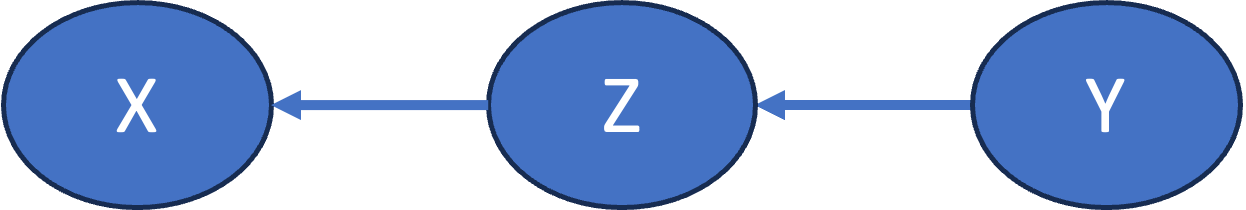
\includegraphics[width = 5cm, height = 1cm]{equiv_1.png}
        \item $P(X,Y,Z) = P(Z)P(X \perp Z)P(Y \perp Z)$
        
        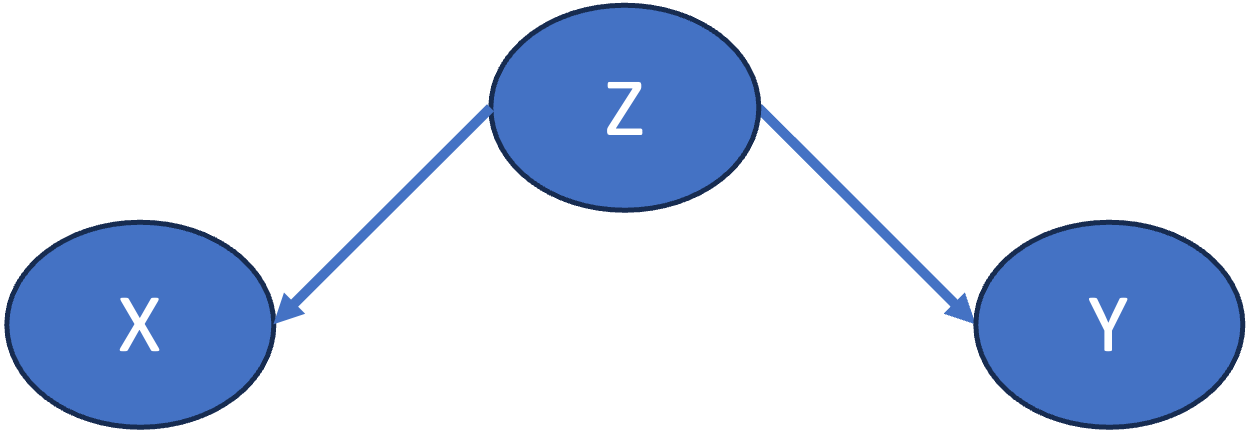
\includegraphics[width = 5cm, height = 2cm]{equiv_2.png}
        \item $P(X,Y,Z) = P(Y)P(Z \perp Y)P(X \perp Z)$
        
        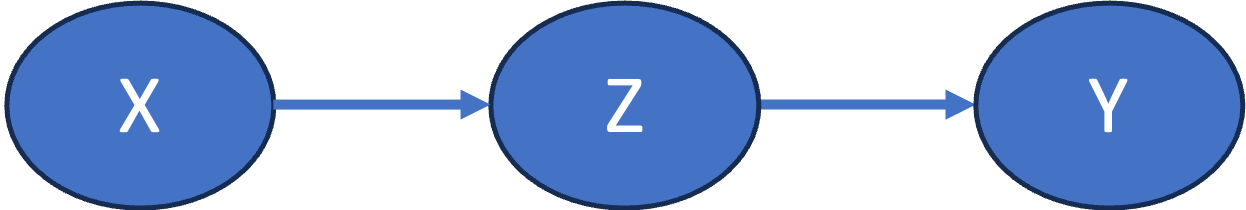
\includegraphics[width = 5cm, height = 1cm]{equiv_3.png}
    \end{itemize}
    \item V-Structure
    
    Suppose we have I(G) = ${X \perp Y}$, $P(X,Y,Z) = P(X)P(Y)P(Z \perp X,Y)$, it cannot be converted to another structure using the bayes rule.

    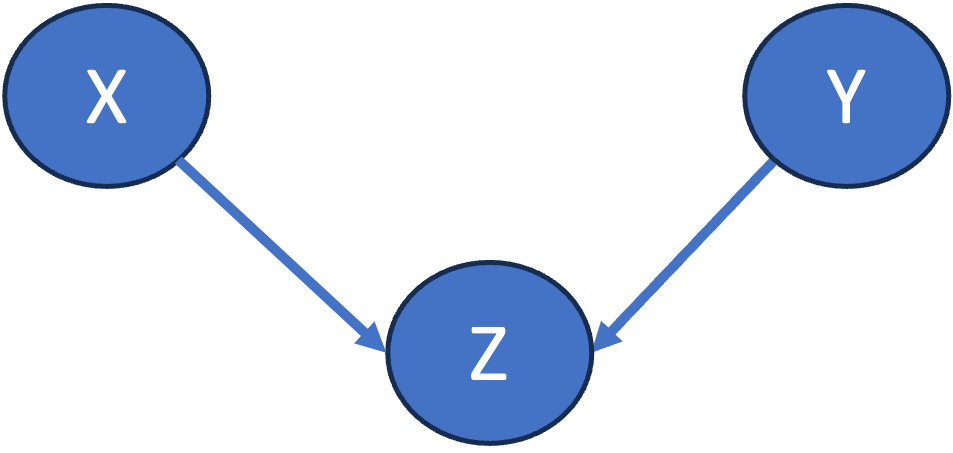
\includegraphics[width = 5cm, height = 2cm]{v_structure.png}

    \item Definition: Independence-equivalence
    
    Two graphs G1 and G2 defined over the same variables are I-equivalent if I(G1) = I(G2). If two graphs have the same skeleton and set of v-structures, then they are i-equivalent.

    \item General trail
    
    In general, the arrows in a trail can be reversed as long as a new v-structure is not produced.

    \item Immorality
    
    A v-structure X -> Z <- Y is an immorality if X and Y are not linked. If there is a link, it is called a covering edge.

    The graphs G1 and G2 are i-equivalent if and only if they have the same skeleton and the same set of immoralities.

    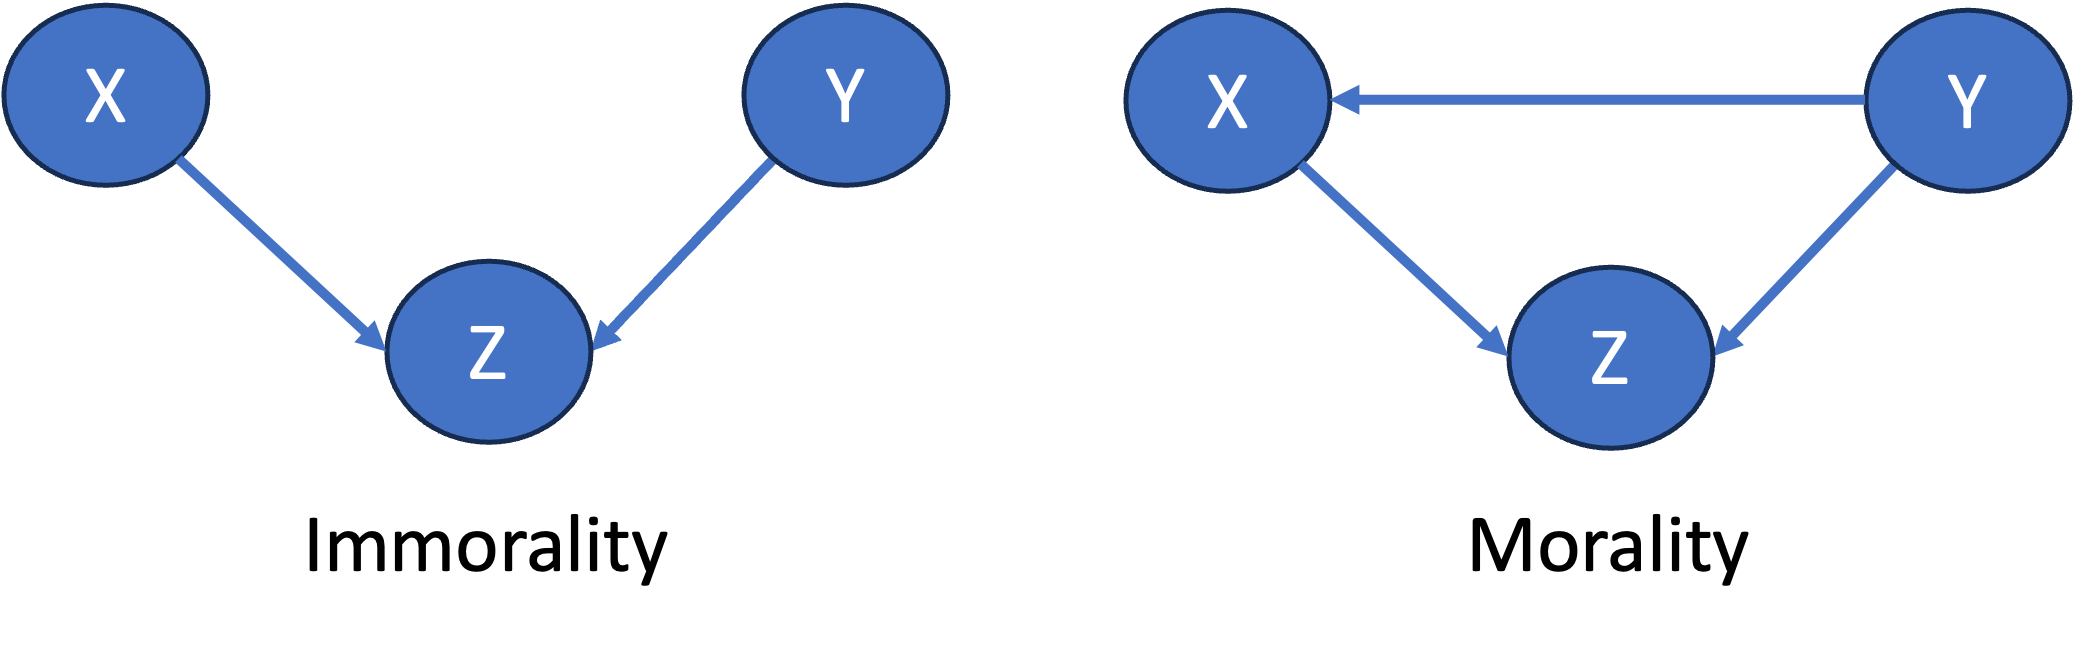
\includegraphics[width = 10cm, height = 3cm]{morality.png}

\end{itemize}

\section{I-equivalence class: PDAG}

\begin{itemize}
    \item Class PDAG of a DAG g is a PDAG that

    \begin{itemize}
        \item has the same skeleton as G
        \item includes a directed edge only if all of the i-equivalent graphs to G also have that directed edge.
    \end{itemize}

\item How to obtain the class PDAG of a DAG G

    \begin{itemize}
        \item obtain the skeleton of G.
        \item find the immoralities of G and draw them in the skeleton.
        \item find the orientations of the other edges by obeying the folloing rules: 1. do not create extra immorality. 2. do not create a directed cycle.
    \end{itemize}

\item Example

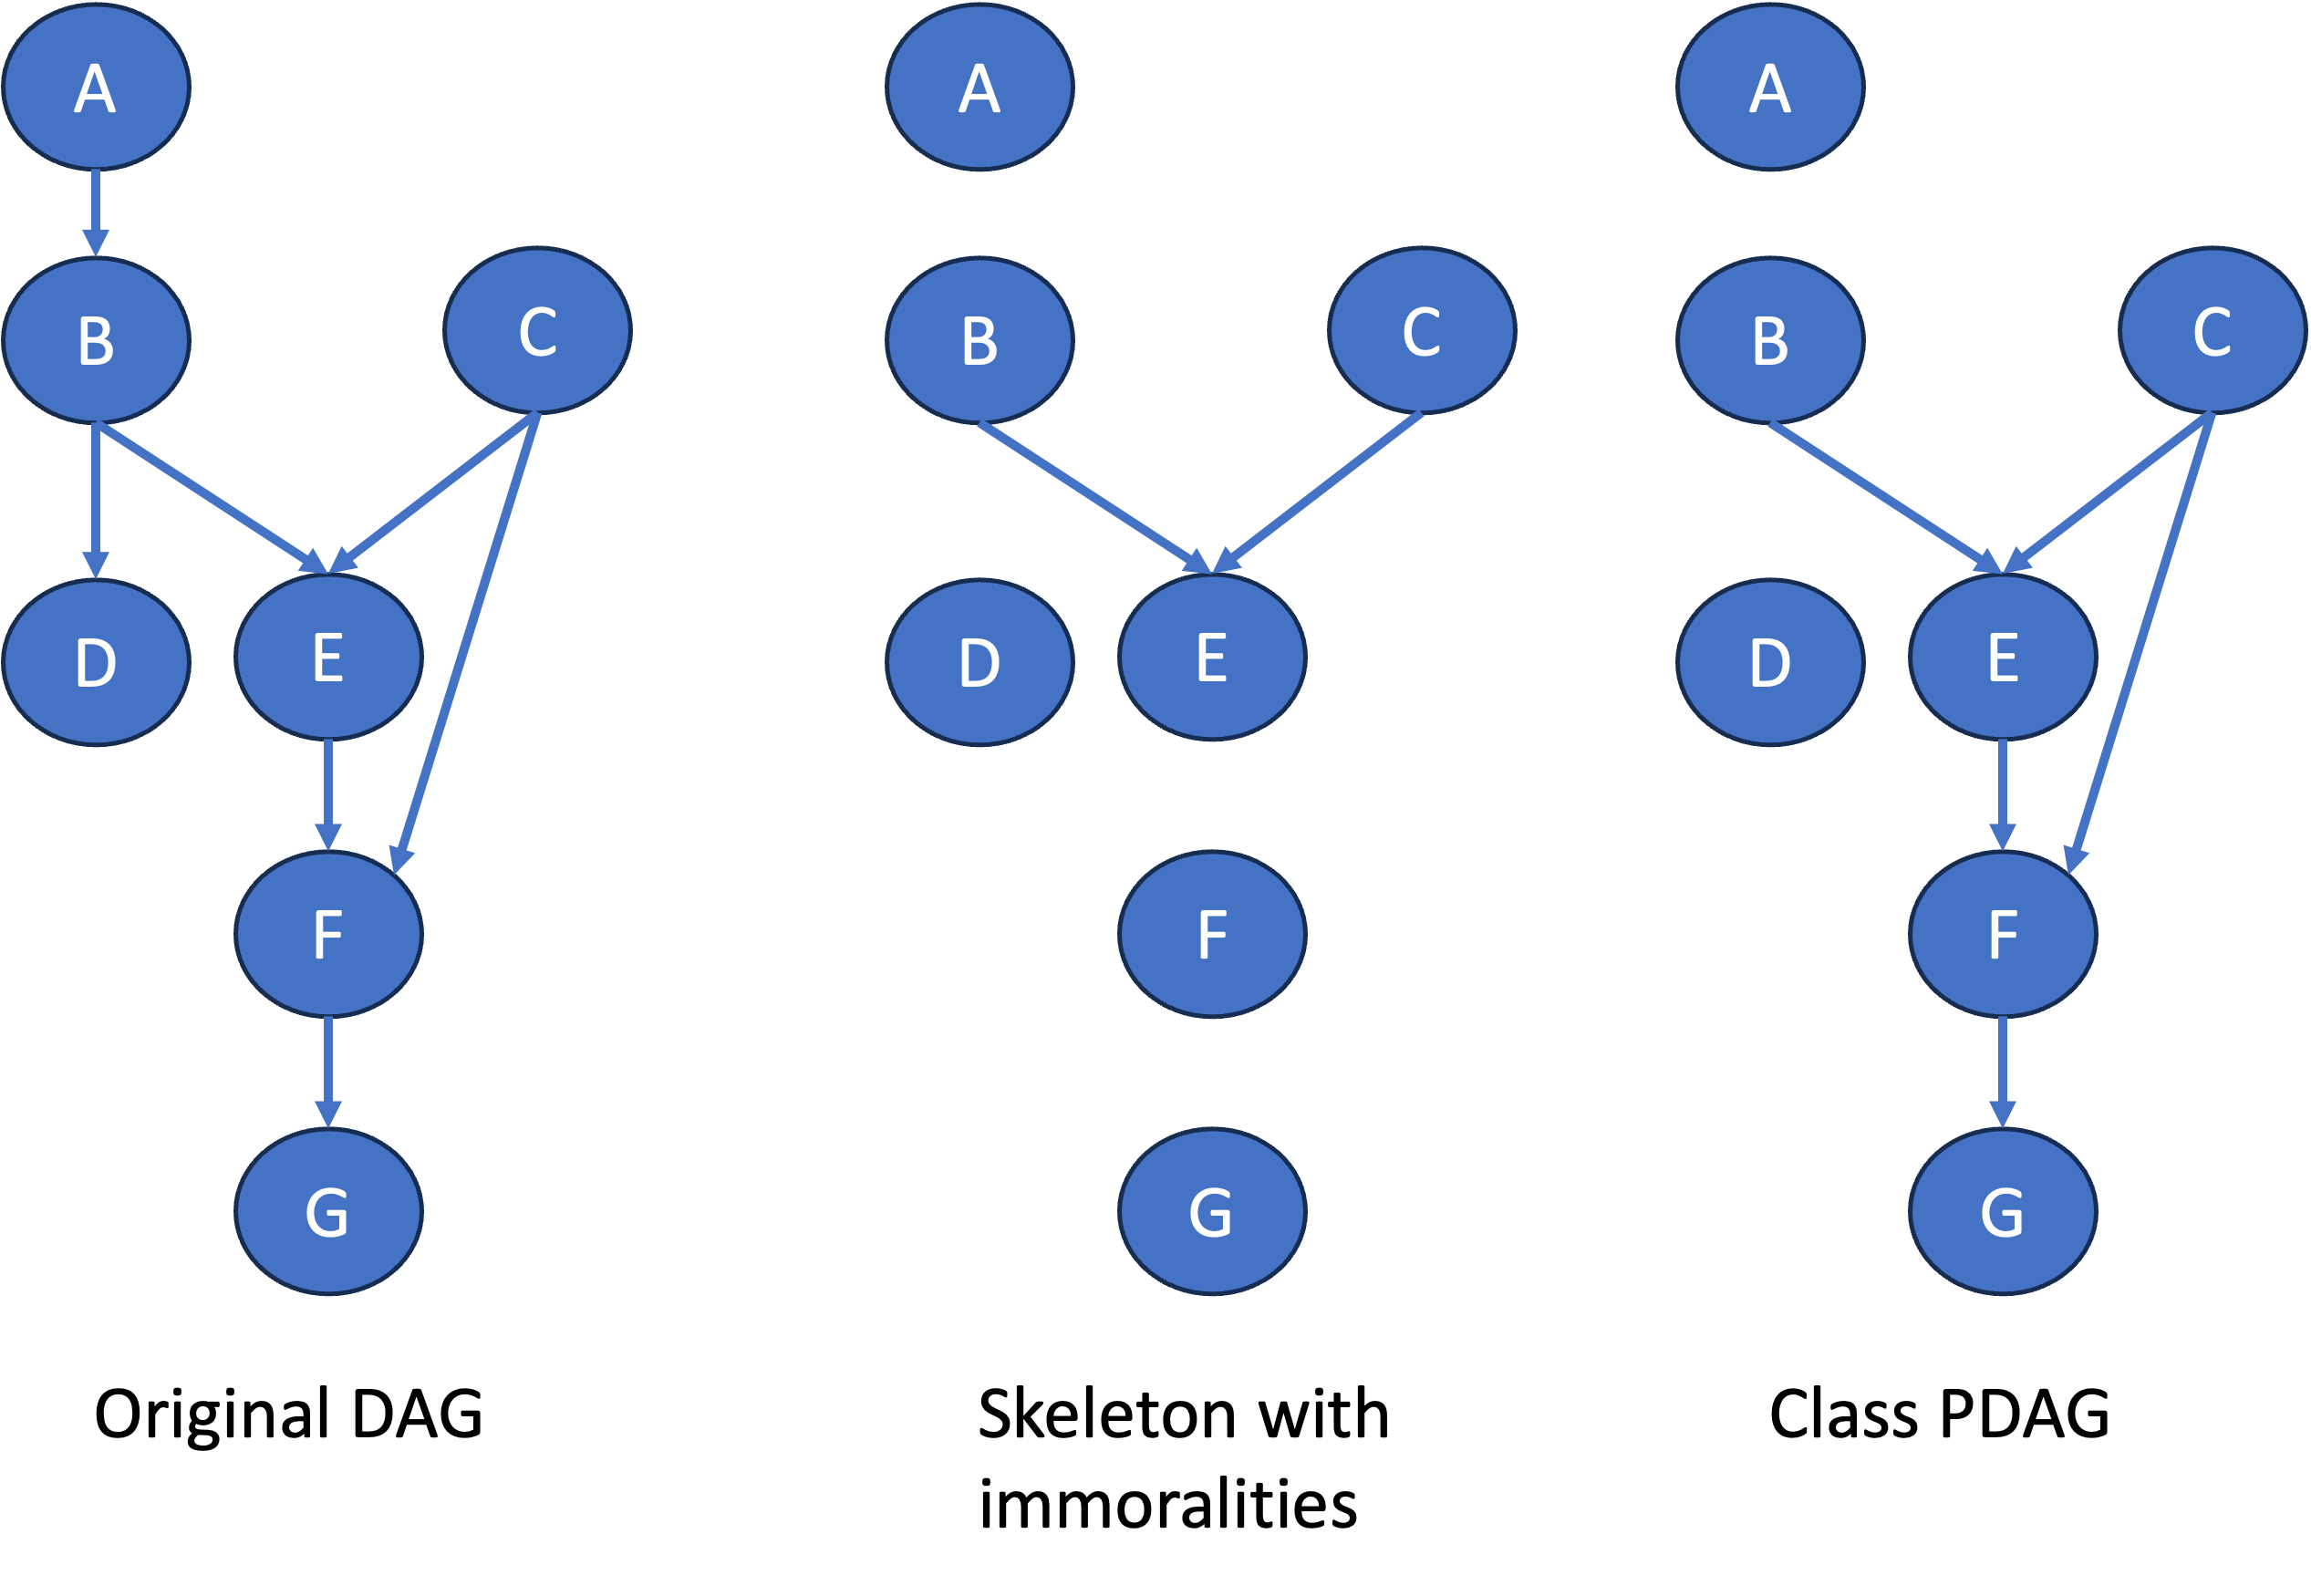
\includegraphics[width = 10cm, height = 7cm]{pdag.png}

\end{itemize}

\section{Summary: What is the Goal?}

The goal is to find from data, the correct factorization of the joint probability distribution. 

\begin{itemize}
    \item First, finding the conditional independence I(P)
    \item For each factorization, we could draw a bayesian nets, and we could write down local independencies $I_{l}^{G}$. If $I_{l}^{G} \subseteq I(P)$, then G is I\_map for P
    \item There could be several i\_map for P, which one to choose? The minimal I-maps
    \item Does P satisfy all global independencies imposed by the minimal I-maps? yes
    \item Do the minimal I-maps satisfy all independencies imposed by P? Are the minimal I-maps a P-map? Depends on I(P)
    \item Is there a class of minimal I-maps? Yes
\end{itemize}

%%------------------------------- chapter ------------------------------------

\chapter{Naive Bayes Model}

In the Covid example, suppose we want to detect the disease type based on the symptoms. What is the simpliest BN that can do this?

Assume Disease class Y = {Allergy, Flu, COVID}

\begin{itemize}
    \item Option 1
    
    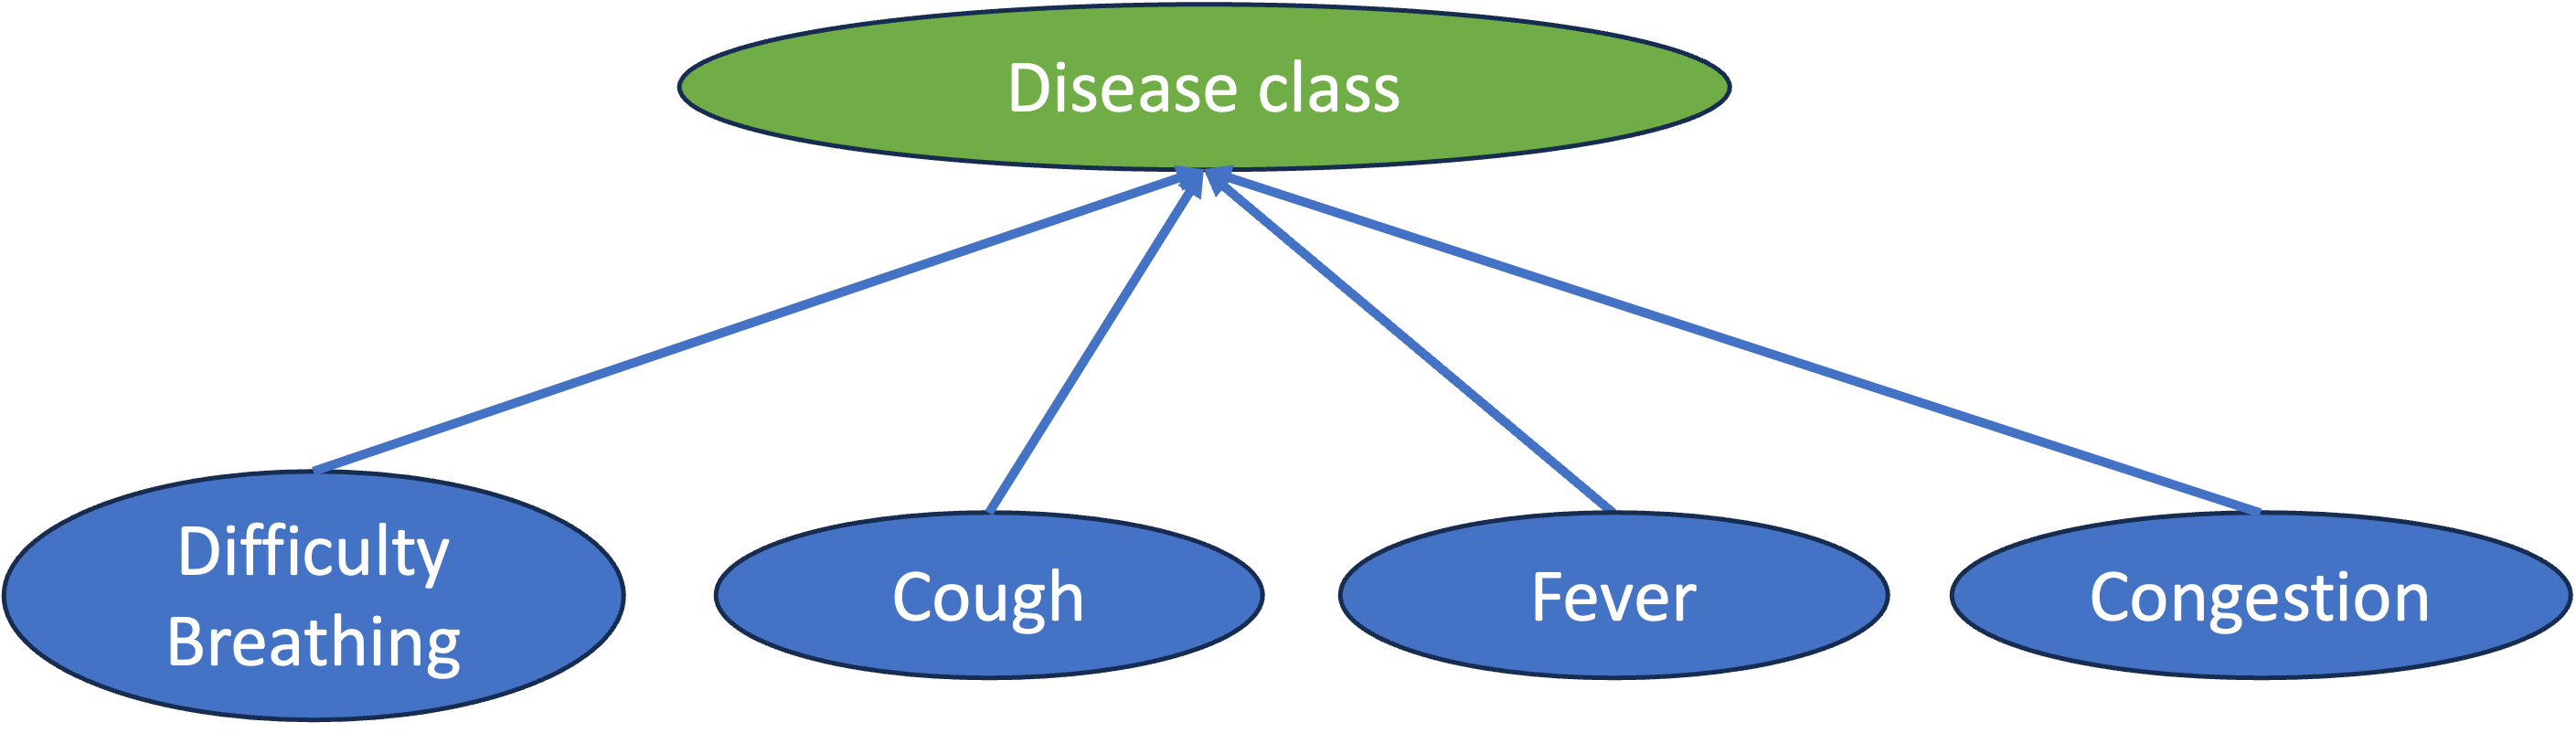
\includegraphics[width = 12cm, height = 3cm]{bay2.png}\\
    This BN will lead to 32 parameters, P(Disease|B,C,F,G).

    \item Option 2
    
    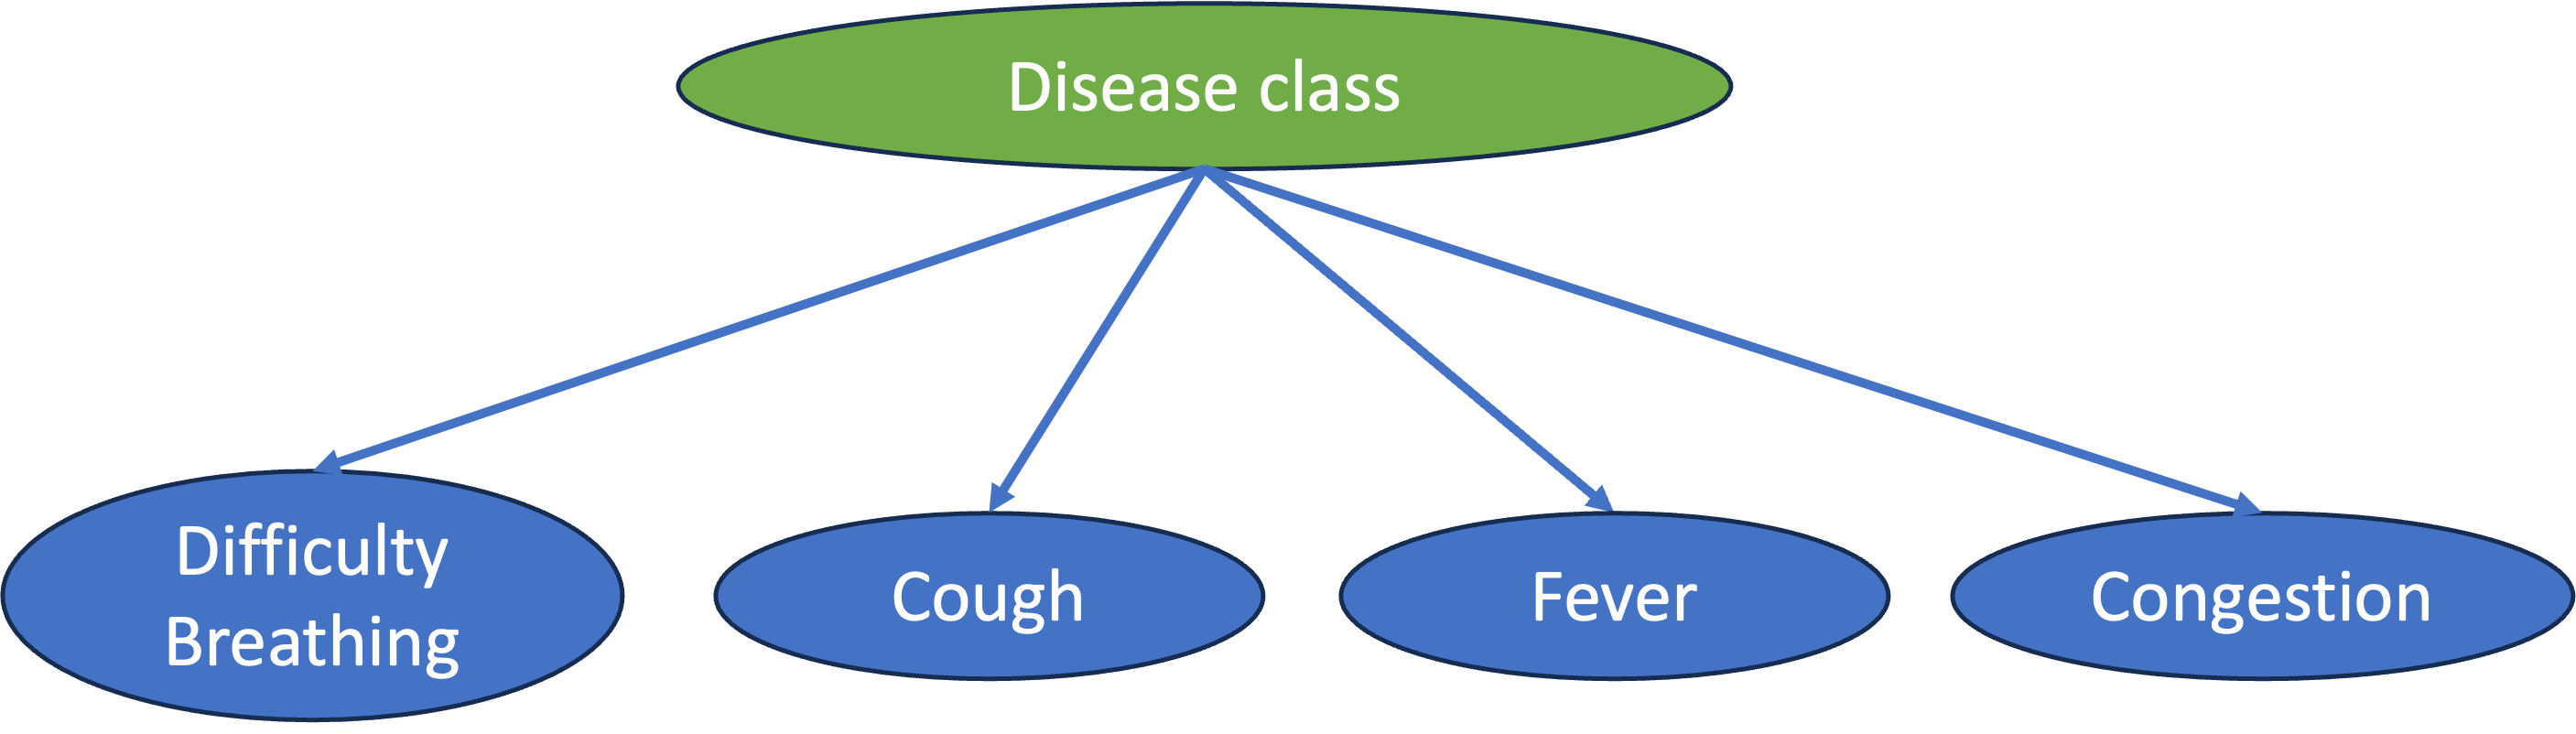
\includegraphics[width = 12cm, height = 3cm]{bay1.png}\\
    This BN will lead to 15 parameters.

    \begin{itemize}
        \item Local dependencies: $I(G) = \{(G \perp F,O,B \mid Y), (F \perp O,G,B \mid Y)$, \\
        $(O \perp F,G,B \mid Y), (B \perp F,O,G \mid Y)\}$
        \item So the symptoms are mutually independent given the disease class.
        \item By specifying the CPDs, we have the probability of each symptoms given the disease.
        \item Total number of params is 15: 2 for Y and 3 for each sympton.
        \item P(Y, X1, \ldots, Xn) are factorized as $P(Y)\prod_{i=1}^{n}P(X_{i} \mid Y)$
        \item With joint probability distribution, we could calculate the probability of each disease given the symptoms.
    \end{itemize}



\end{itemize}





\end{document}
